% Options for packages loaded elsewhere
\PassOptionsToPackage{unicode}{hyperref}
\PassOptionsToPackage{hyphens}{url}
\documentclass[
]{article}
\usepackage{xcolor}
\usepackage[margin=1in]{geometry}
\usepackage{amsmath,amssymb}
\setcounter{secnumdepth}{-\maxdimen} % remove section numbering
\usepackage{iftex}
\ifPDFTeX
  \usepackage[T1]{fontenc}
  \usepackage[utf8]{inputenc}
  \usepackage{textcomp} % provide euro and other symbols
\else % if luatex or xetex
  \usepackage{unicode-math} % this also loads fontspec
  \defaultfontfeatures{Scale=MatchLowercase}
  \defaultfontfeatures[\rmfamily]{Ligatures=TeX,Scale=1}
\fi
\usepackage{lmodern}
\ifPDFTeX\else
  % xetex/luatex font selection
\fi
% Use upquote if available, for straight quotes in verbatim environments
\IfFileExists{upquote.sty}{\usepackage{upquote}}{}
\IfFileExists{microtype.sty}{% use microtype if available
  \usepackage[]{microtype}
  \UseMicrotypeSet[protrusion]{basicmath} % disable protrusion for tt fonts
}{}
\makeatletter
\@ifundefined{KOMAClassName}{% if non-KOMA class
  \IfFileExists{parskip.sty}{%
    \usepackage{parskip}
  }{% else
    \setlength{\parindent}{0pt}
    \setlength{\parskip}{6pt plus 2pt minus 1pt}}
}{% if KOMA class
  \KOMAoptions{parskip=half}}
\makeatother
\usepackage{color}
\usepackage{fancyvrb}
\newcommand{\VerbBar}{|}
\newcommand{\VERB}{\Verb[commandchars=\\\{\}]}
\DefineVerbatimEnvironment{Highlighting}{Verbatim}{commandchars=\\\{\}}
% Add ',fontsize=\small' for more characters per line
\usepackage{framed}
\definecolor{shadecolor}{RGB}{248,248,248}
\newenvironment{Shaded}{\begin{snugshade}}{\end{snugshade}}
\newcommand{\AlertTok}[1]{\textcolor[rgb]{0.94,0.16,0.16}{#1}}
\newcommand{\AnnotationTok}[1]{\textcolor[rgb]{0.56,0.35,0.01}{\textbf{\textit{#1}}}}
\newcommand{\AttributeTok}[1]{\textcolor[rgb]{0.13,0.29,0.53}{#1}}
\newcommand{\BaseNTok}[1]{\textcolor[rgb]{0.00,0.00,0.81}{#1}}
\newcommand{\BuiltInTok}[1]{#1}
\newcommand{\CharTok}[1]{\textcolor[rgb]{0.31,0.60,0.02}{#1}}
\newcommand{\CommentTok}[1]{\textcolor[rgb]{0.56,0.35,0.01}{\textit{#1}}}
\newcommand{\CommentVarTok}[1]{\textcolor[rgb]{0.56,0.35,0.01}{\textbf{\textit{#1}}}}
\newcommand{\ConstantTok}[1]{\textcolor[rgb]{0.56,0.35,0.01}{#1}}
\newcommand{\ControlFlowTok}[1]{\textcolor[rgb]{0.13,0.29,0.53}{\textbf{#1}}}
\newcommand{\DataTypeTok}[1]{\textcolor[rgb]{0.13,0.29,0.53}{#1}}
\newcommand{\DecValTok}[1]{\textcolor[rgb]{0.00,0.00,0.81}{#1}}
\newcommand{\DocumentationTok}[1]{\textcolor[rgb]{0.56,0.35,0.01}{\textbf{\textit{#1}}}}
\newcommand{\ErrorTok}[1]{\textcolor[rgb]{0.64,0.00,0.00}{\textbf{#1}}}
\newcommand{\ExtensionTok}[1]{#1}
\newcommand{\FloatTok}[1]{\textcolor[rgb]{0.00,0.00,0.81}{#1}}
\newcommand{\FunctionTok}[1]{\textcolor[rgb]{0.13,0.29,0.53}{\textbf{#1}}}
\newcommand{\ImportTok}[1]{#1}
\newcommand{\InformationTok}[1]{\textcolor[rgb]{0.56,0.35,0.01}{\textbf{\textit{#1}}}}
\newcommand{\KeywordTok}[1]{\textcolor[rgb]{0.13,0.29,0.53}{\textbf{#1}}}
\newcommand{\NormalTok}[1]{#1}
\newcommand{\OperatorTok}[1]{\textcolor[rgb]{0.81,0.36,0.00}{\textbf{#1}}}
\newcommand{\OtherTok}[1]{\textcolor[rgb]{0.56,0.35,0.01}{#1}}
\newcommand{\PreprocessorTok}[1]{\textcolor[rgb]{0.56,0.35,0.01}{\textit{#1}}}
\newcommand{\RegionMarkerTok}[1]{#1}
\newcommand{\SpecialCharTok}[1]{\textcolor[rgb]{0.81,0.36,0.00}{\textbf{#1}}}
\newcommand{\SpecialStringTok}[1]{\textcolor[rgb]{0.31,0.60,0.02}{#1}}
\newcommand{\StringTok}[1]{\textcolor[rgb]{0.31,0.60,0.02}{#1}}
\newcommand{\VariableTok}[1]{\textcolor[rgb]{0.00,0.00,0.00}{#1}}
\newcommand{\VerbatimStringTok}[1]{\textcolor[rgb]{0.31,0.60,0.02}{#1}}
\newcommand{\WarningTok}[1]{\textcolor[rgb]{0.56,0.35,0.01}{\textbf{\textit{#1}}}}
\usepackage{longtable,booktabs,array}
\usepackage{calc} % for calculating minipage widths
% Correct order of tables after \paragraph or \subparagraph
\usepackage{etoolbox}
\makeatletter
\patchcmd\longtable{\par}{\if@noskipsec\mbox{}\fi\par}{}{}
\makeatother
% Allow footnotes in longtable head/foot
\IfFileExists{footnotehyper.sty}{\usepackage{footnotehyper}}{\usepackage{footnote}}
\makesavenoteenv{longtable}
\usepackage{graphicx}
\makeatletter
\newsavebox\pandoc@box
\newcommand*\pandocbounded[1]{% scales image to fit in text height/width
  \sbox\pandoc@box{#1}%
  \Gscale@div\@tempa{\textheight}{\dimexpr\ht\pandoc@box+\dp\pandoc@box\relax}%
  \Gscale@div\@tempb{\linewidth}{\wd\pandoc@box}%
  \ifdim\@tempb\p@<\@tempa\p@\let\@tempa\@tempb\fi% select the smaller of both
  \ifdim\@tempa\p@<\p@\scalebox{\@tempa}{\usebox\pandoc@box}%
  \else\usebox{\pandoc@box}%
  \fi%
}
% Set default figure placement to htbp
\def\fps@figure{htbp}
\makeatother
\setlength{\emergencystretch}{3em} % prevent overfull lines
\providecommand{\tightlist}{%
  \setlength{\itemsep}{0pt}\setlength{\parskip}{0pt}}
\usepackage{booktabs}
\usepackage{longtable}
\usepackage{array}
\usepackage{multirow}
\usepackage{wrapfig}
\usepackage{float}
\usepackage{colortbl}
\usepackage{pdflscape}
\usepackage{tabu}
\usepackage{threeparttable}
\usepackage{threeparttablex}
\usepackage[normalem]{ulem}
\usepackage{makecell}
\usepackage{xcolor}
\usepackage{bookmark}
\IfFileExists{xurl.sty}{\usepackage{xurl}}{} % add URL line breaks if available
\urlstyle{same}
\hypersetup{
  pdftitle={DATA621\_Homework3\_Group2},
  pdfauthor={Group2},
  hidelinks,
  pdfcreator={LaTeX via pandoc}}

\title{DATA621\_Homework3\_Group2}
\author{Group2}
\date{2025-04-06}

\begin{document}
\maketitle

{
\setcounter{tocdepth}{5}
\tableofcontents
}
\subsection{Overview}\label{overview}

In this homework assignment, you will explore, analyze and model a data
set containing information on crime for various neighborhoods of a major
city. Each record has a response variable indicating whether or not the
crime rate is above the median crime rate (1) or not (0). Your objective
is to build a binary logistic regression model on the training data set
to predict whether the neighborhood will be at risk for high crime
levels. You will provide classifications and probabilities for the
evaluation data set using your binary logistic regression model. You can
only use the variables given to you (or, variables that you derive from
the variables provided). Below is a short description of the variables
of interest in the data set: • zn: proportion of residential land zoned
for large lots (over 25000 square feet) (predictor variable) • indus:
proportion of non-retail business acres per suburb (predictor variable)
• chas: a dummy var. for whether the suburb borders the Charles River
(1) or not (0) (predictor variable) • nox: nitrogen oxides concentration
(parts per 10 million) (predictor variable) • rm: average number of
rooms per dwelling (predictor variable) • age: proportion of
owner-occupied units built prior to 1940 (predictor variable) • dis:
weighted mean of distances to five Boston employment centers (predictor
variable) • rad: index of accessibility to radial highways (predictor
variable) • tax: full-value property-tax rate per \$10,000 (predictor
variable) • ptratio: pupil-teacher ratio by town (predictor variable) •
lstat: lower status of the population (percent) (predictor variable) •
medv: median value of owner-occupied homes in \$1000s (predictor
variable) • target: whether the crime rate is above the median crime
rate (1) or not (0) (response variable)

\subsection{Deliverables:}\label{deliverables}

• A write-up submitted in PDF format. Your write-up should have four
sections. Each one is described below. You may assume you are addressing
me as a fellow data scientist, so do not need to shy away from technical
details. • Assigned prediction (probabilities, classifications) for the
evaluation data set. Use 0.5 threshold. Include your R statistical
programming code in an Appendix.

\subsubsection{1. DATA EXPLORATION (25
Points)}\label{data-exploration-25-points}

Describe the size and the variables in the crime training data set.
Consider that too much detail will cause a manager to lose interest
while too little detail will make the manager consider that you aren't
doing your job. Some suggestions are given below. Please do NOT treat
this as a check list of things to do to complete the assignment. You
should have your own thoughts on what to tell the boss. These are just
ideas. a. Mean / Standard Deviation / Median b. Bar Chart or Box Plot of
the data c.~Is the data correlated to the target variable (or to other
variables?) d.~Are any of the variables missing and need to be
imputed/``fixed''?

\paragraph{DATA EXPLORATION WRITE UP}\label{data-exploration-write-up}

The training dataset consists of 466 observations and 14 variables,
including 13 predictors and a binary response variable. The binary
response variable, target, indicates that a neighborhood's crime rate
exceeds the citywide median (a value of 1) or not ( a value of 0). A
null-check confirmed that there are no missing values in the dataset, so
no imputation or data cleansing was necessary at this stage.

Basic summary statistics reveal that the variables like zn, tax, and age
exhibit wide ranges seemingly from 0 to 100 or more. Columns such as
indus, nox, lstat, medv, rad and dis have smaller ranges. Looking
specifically at some variable, zn, which is the proportion of
residential land zoned for large lots, ranges from 0 to 100. The data
has a median of 0 and a mean of 11.58. This shows that many
neighborhoods have minimal or no large-lot zoning. Another variable, age
, which shows the proportion of homes built before 1940, has a mean of
68.37 and a median of 77.15, suggesting a majority of the housing stock
is relatively old.

Leveraging both box plots for each variable compared to the target
variable, along with a larger ggpairs plot, there were relationships
between the data columns observed.

Firstly, take a look at the ggpairs plot below. This plot revealed
several meaningful correlations and patterns. A strong negative
correlation exists between zn and both indus and nox. This implies areas
zoned for spacious residential use are less likely to host industrial
development and experience fewer nitrogen oxide emissions. The zn
variable also negatively correlates with age. This could indicate larger
residential lots are more common in newer developments. Indus, nox, and
age are positively correlated with one another, which could mean that
older neighborhoods are more industrial and environmentally burdened.
Additionally, a strong negative relationship between the age and rm
variables was seen, implying that older buildings are generally smaller
than newer ones. The distance to employment centers, covered by the dis
variable, negatively correlates with nox, age, and indus. The dis
variable, however, has a positive relationship with zn. This may mean
that larger residential zoning, are more suburban type developments not
near industrialized more urban / downtown environments. Lastly, the
lstat variable, which looks at the proportion of lower status of the
population, is negatively related to zn, rm and dis. Lstat is positively
correlated with indus, nox, and age. This makes sense as older, less
industrialized, more suburban areas would tend to be of higher status.

\pandocbounded{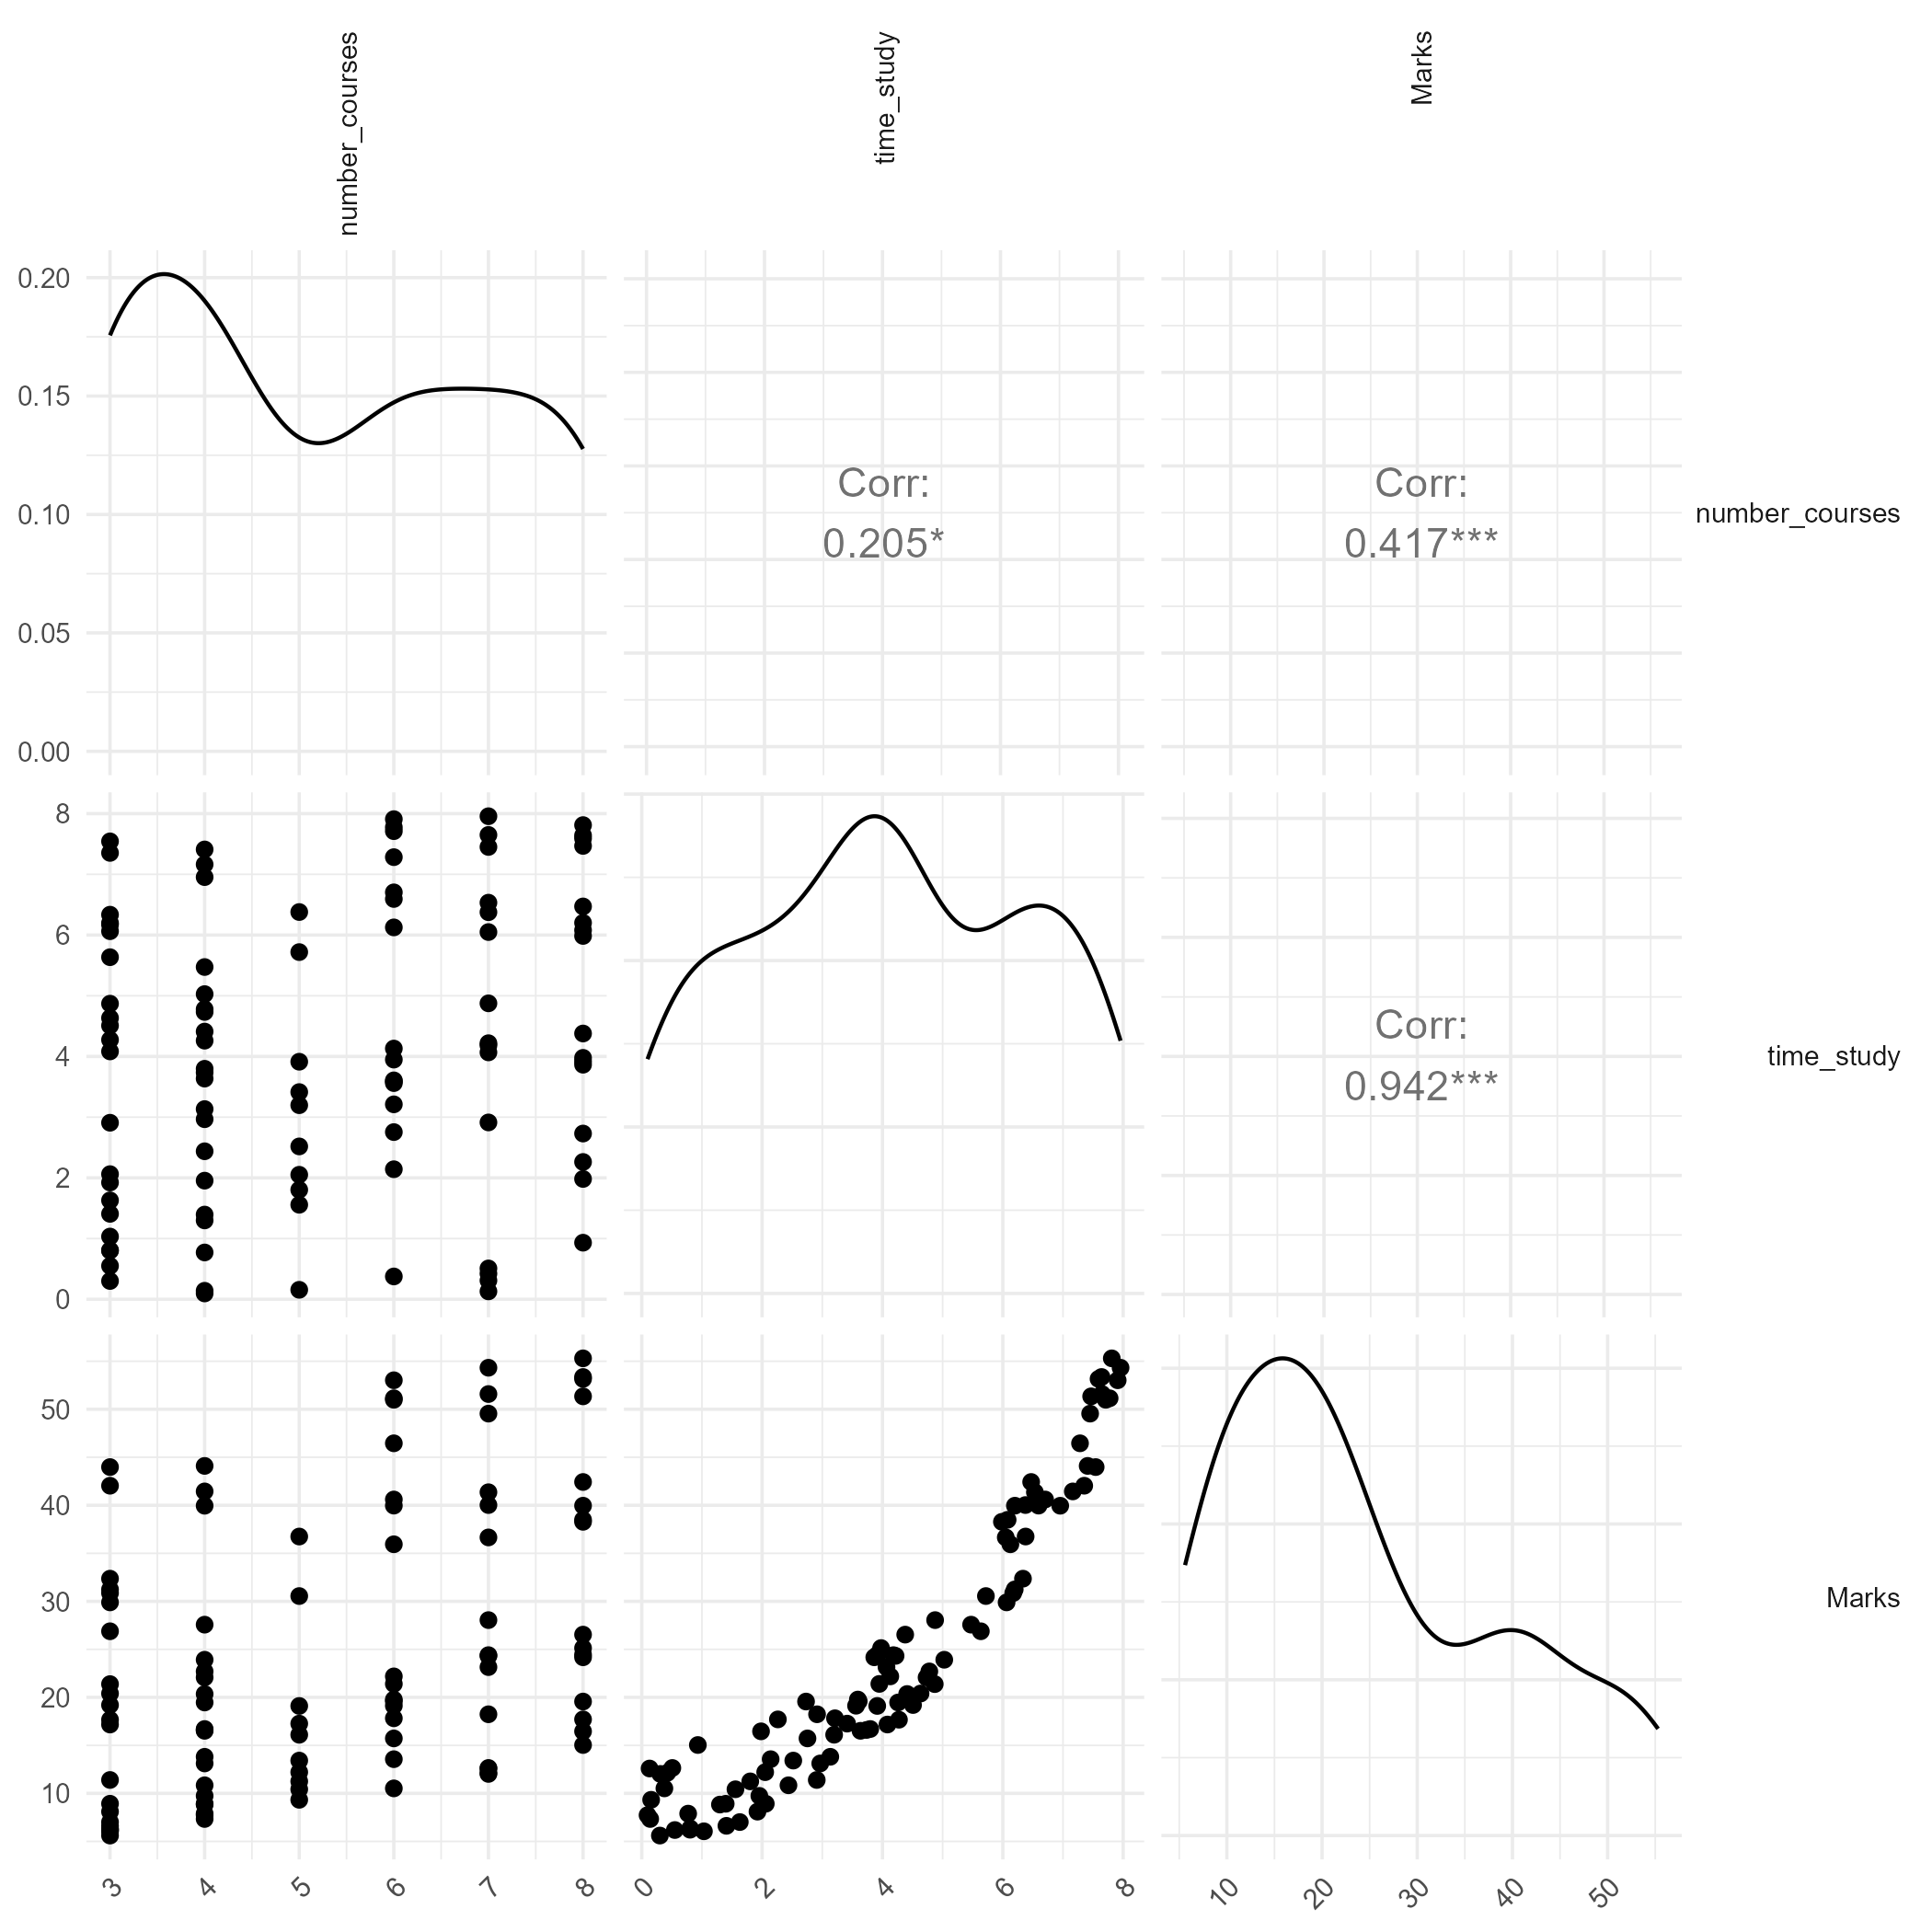
\includegraphics[keepaspectratio]{https://raw.githubusercontent.com/jhnboyy/CUNY_SPS_WORK/refs/heads/main/Spring2025/DATA621/DATA621_Homework3/images/ggpairs_plot.png}}
Now looking at the box plots (below) charted for each variable to gauge
the relationship to the target variable of crime level, there were take
aways here. These takeways can be seen in the following summary table:

\begin{longtable}[]{@{}
  >{\raggedright\arraybackslash}p{(\linewidth - 4\tabcolsep) * \real{0.2466}}
  >{\raggedright\arraybackslash}p{(\linewidth - 4\tabcolsep) * \real{0.5068}}
  >{\raggedright\arraybackslash}p{(\linewidth - 4\tabcolsep) * \real{0.2466}}@{}}
\toprule\noalign{}
\begin{minipage}[b]{\linewidth}\raggedright
Variable
\end{minipage} & \begin{minipage}[b]{\linewidth}\raggedright
Relationship to Crime (Target = 1)
\end{minipage} & \begin{minipage}[b]{\linewidth}\raggedright
Insight
\end{minipage} \\
\midrule\noalign{}
\endhead
\bottomrule\noalign{}
\endlastfoot
\texttt{zn} & Lower values → Higher crime & Less residential zoning is
linked to high crime \\
\texttt{indus} & Higher values → Higher crime & More industrial areas
tend to have higher crime \\
\texttt{nox} & Higher values → Higher crime & Pollution correlates with
higher crime rates \\
\texttt{rm} & No clear pattern & Number of rooms not strongly
associated \\
\texttt{age} & Higher values → Higher crime & Older buildings correlate
with higher crime \\
\texttt{dis} & Lower values → Higher crime & Areas closer to employment
centers have more crime \\
\texttt{rad} & Higher values → Higher crime & Greater radial highway
access correlated to higher crime \\
\texttt{tax} & Higher values → Higher crime & High tax correlated higher
crime. \\
\texttt{ptratio} & Slightly higher values → Higher crime & Weak trend,
possibly related to school quality \\
\texttt{lstat} & Slightly higher values → Higher crime & Larger lower
status proportion linked to higher crime \\
\texttt{medv} & Slightly lower values → Higher crime & Lower median
owner-occupied home values associated with high crime \\
\end{longtable}

\pandocbounded{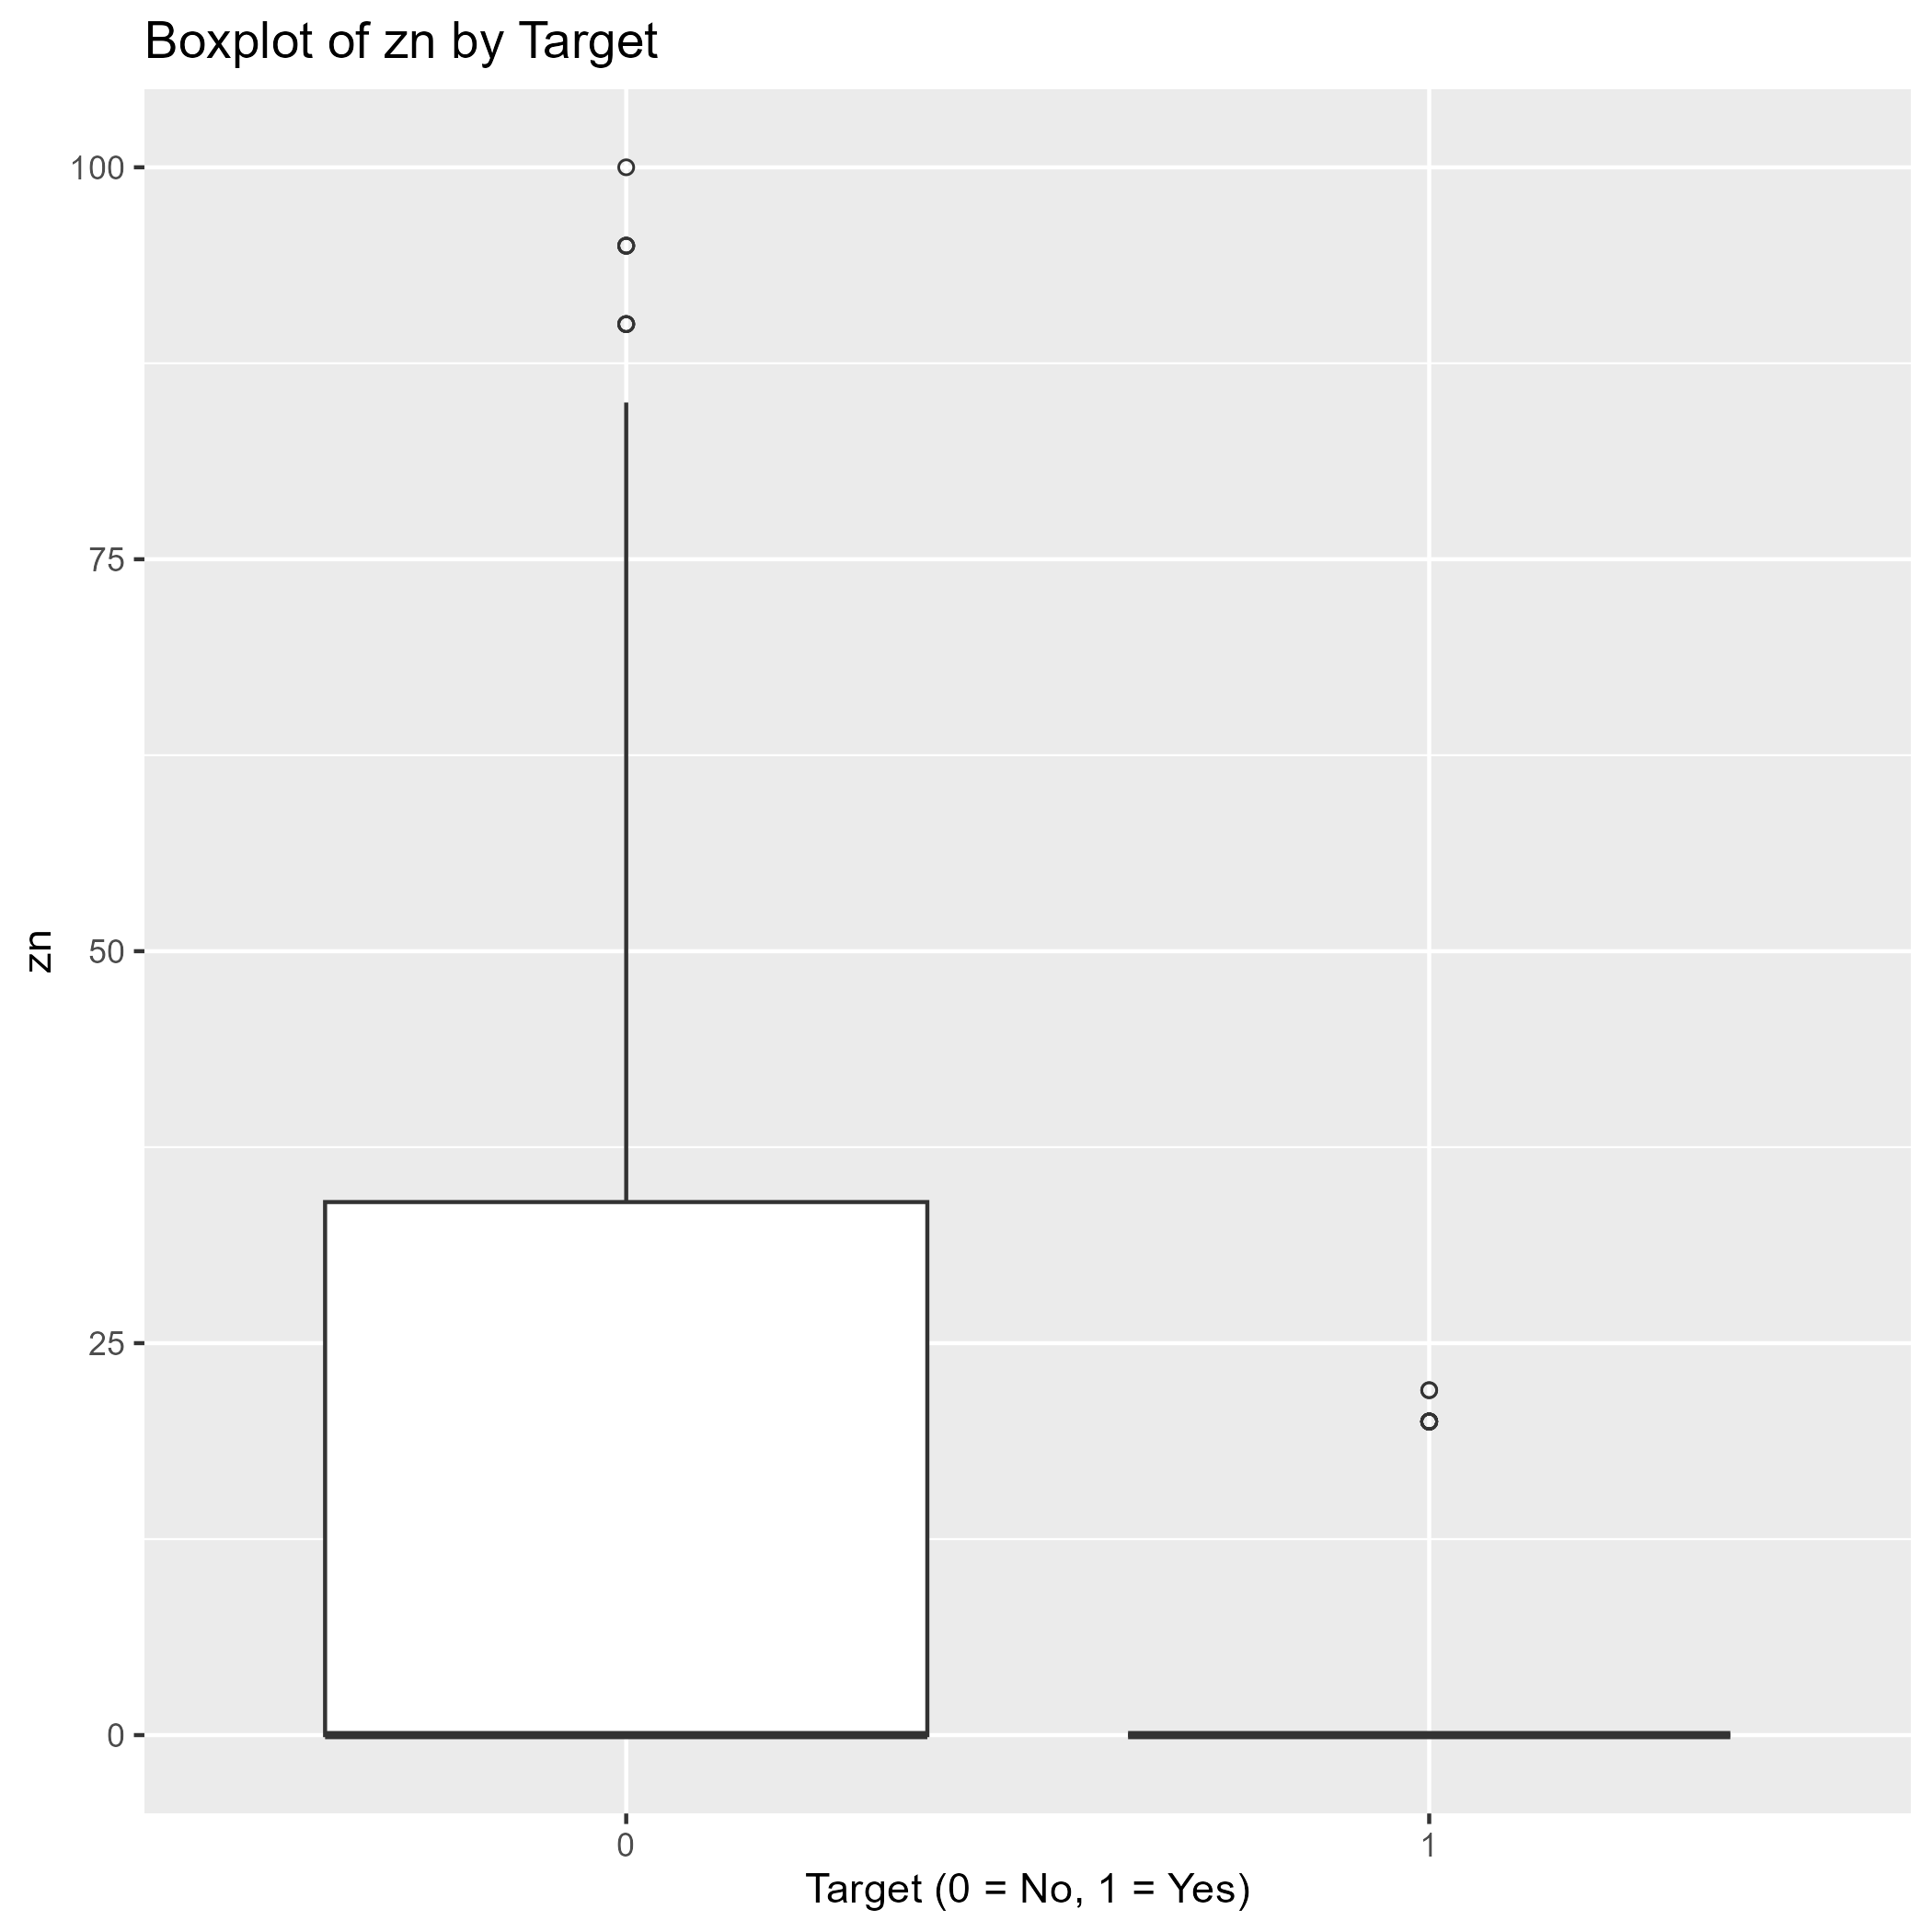
\includegraphics[keepaspectratio]{https://raw.githubusercontent.com/jhnboyy/CUNY_SPS_WORK/refs/heads/main/Spring2025/DATA621/DATA621_Homework3/images/Boxplotzn_plot.png}}
\pandocbounded{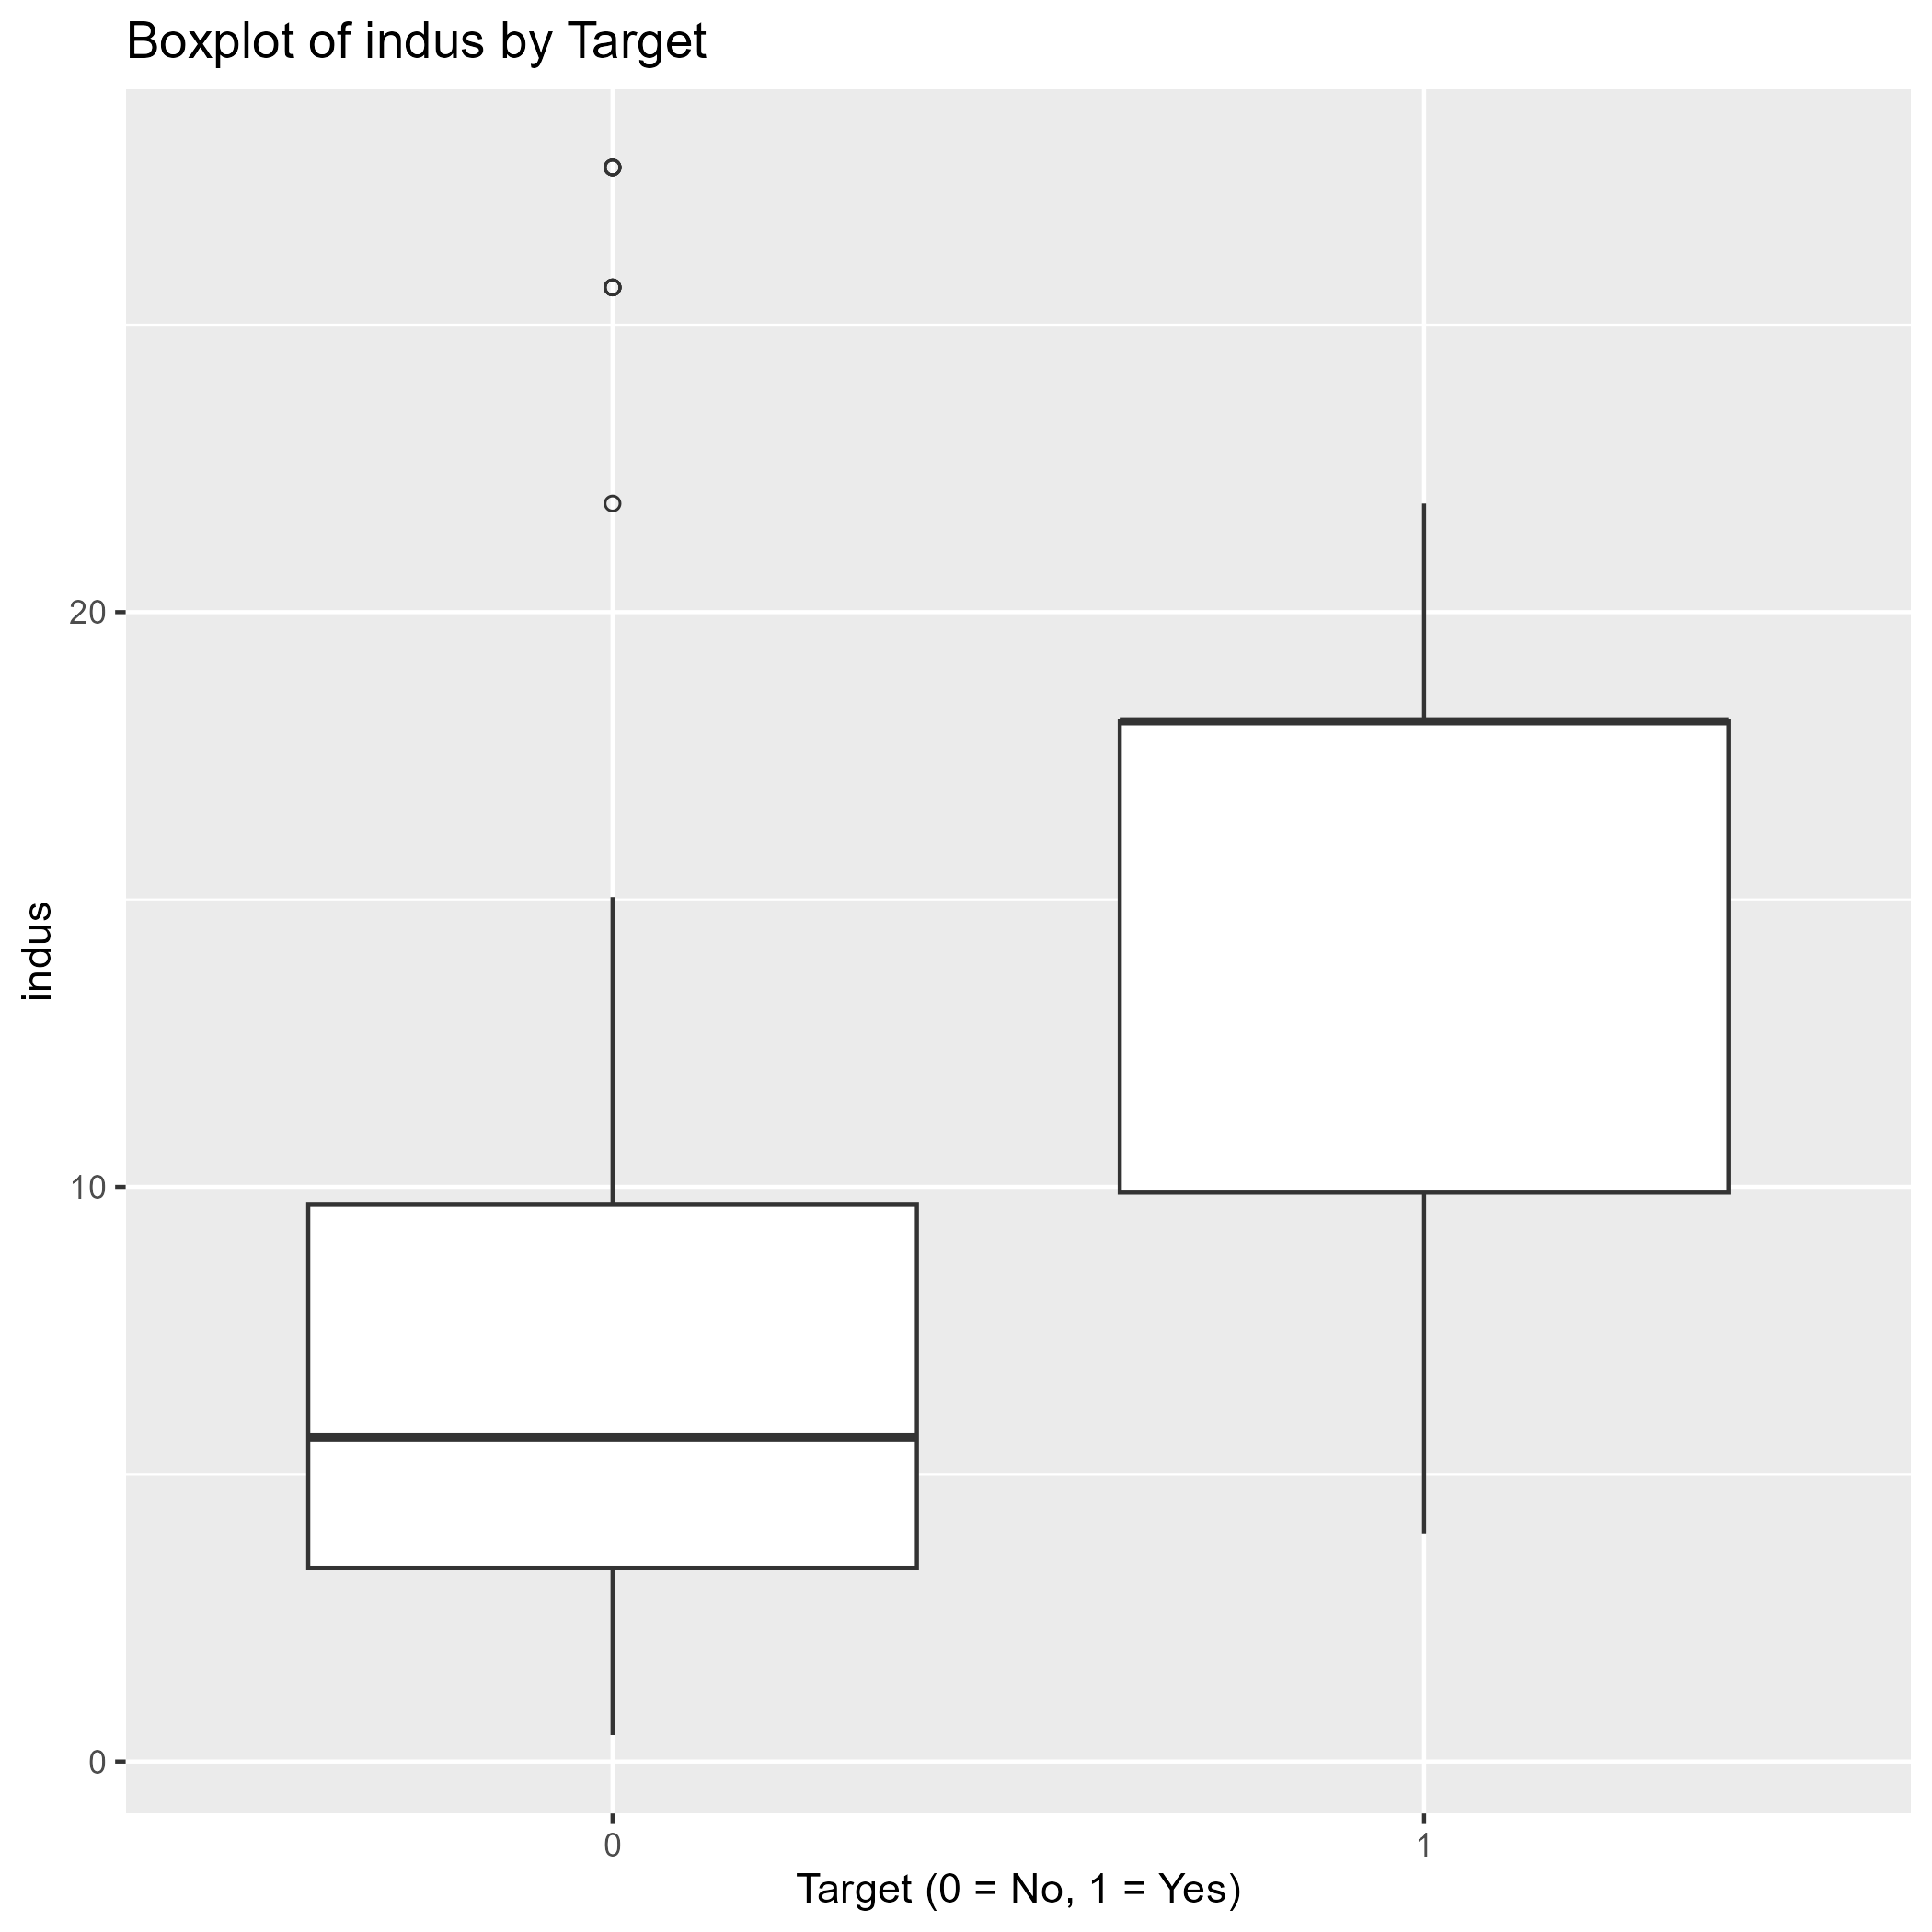
\includegraphics[keepaspectratio]{https://raw.githubusercontent.com/jhnboyy/CUNY_SPS_WORK/refs/heads/main/Spring2025/DATA621/DATA621_Homework3/images/Boxplotindus_plot.png}}
\pandocbounded{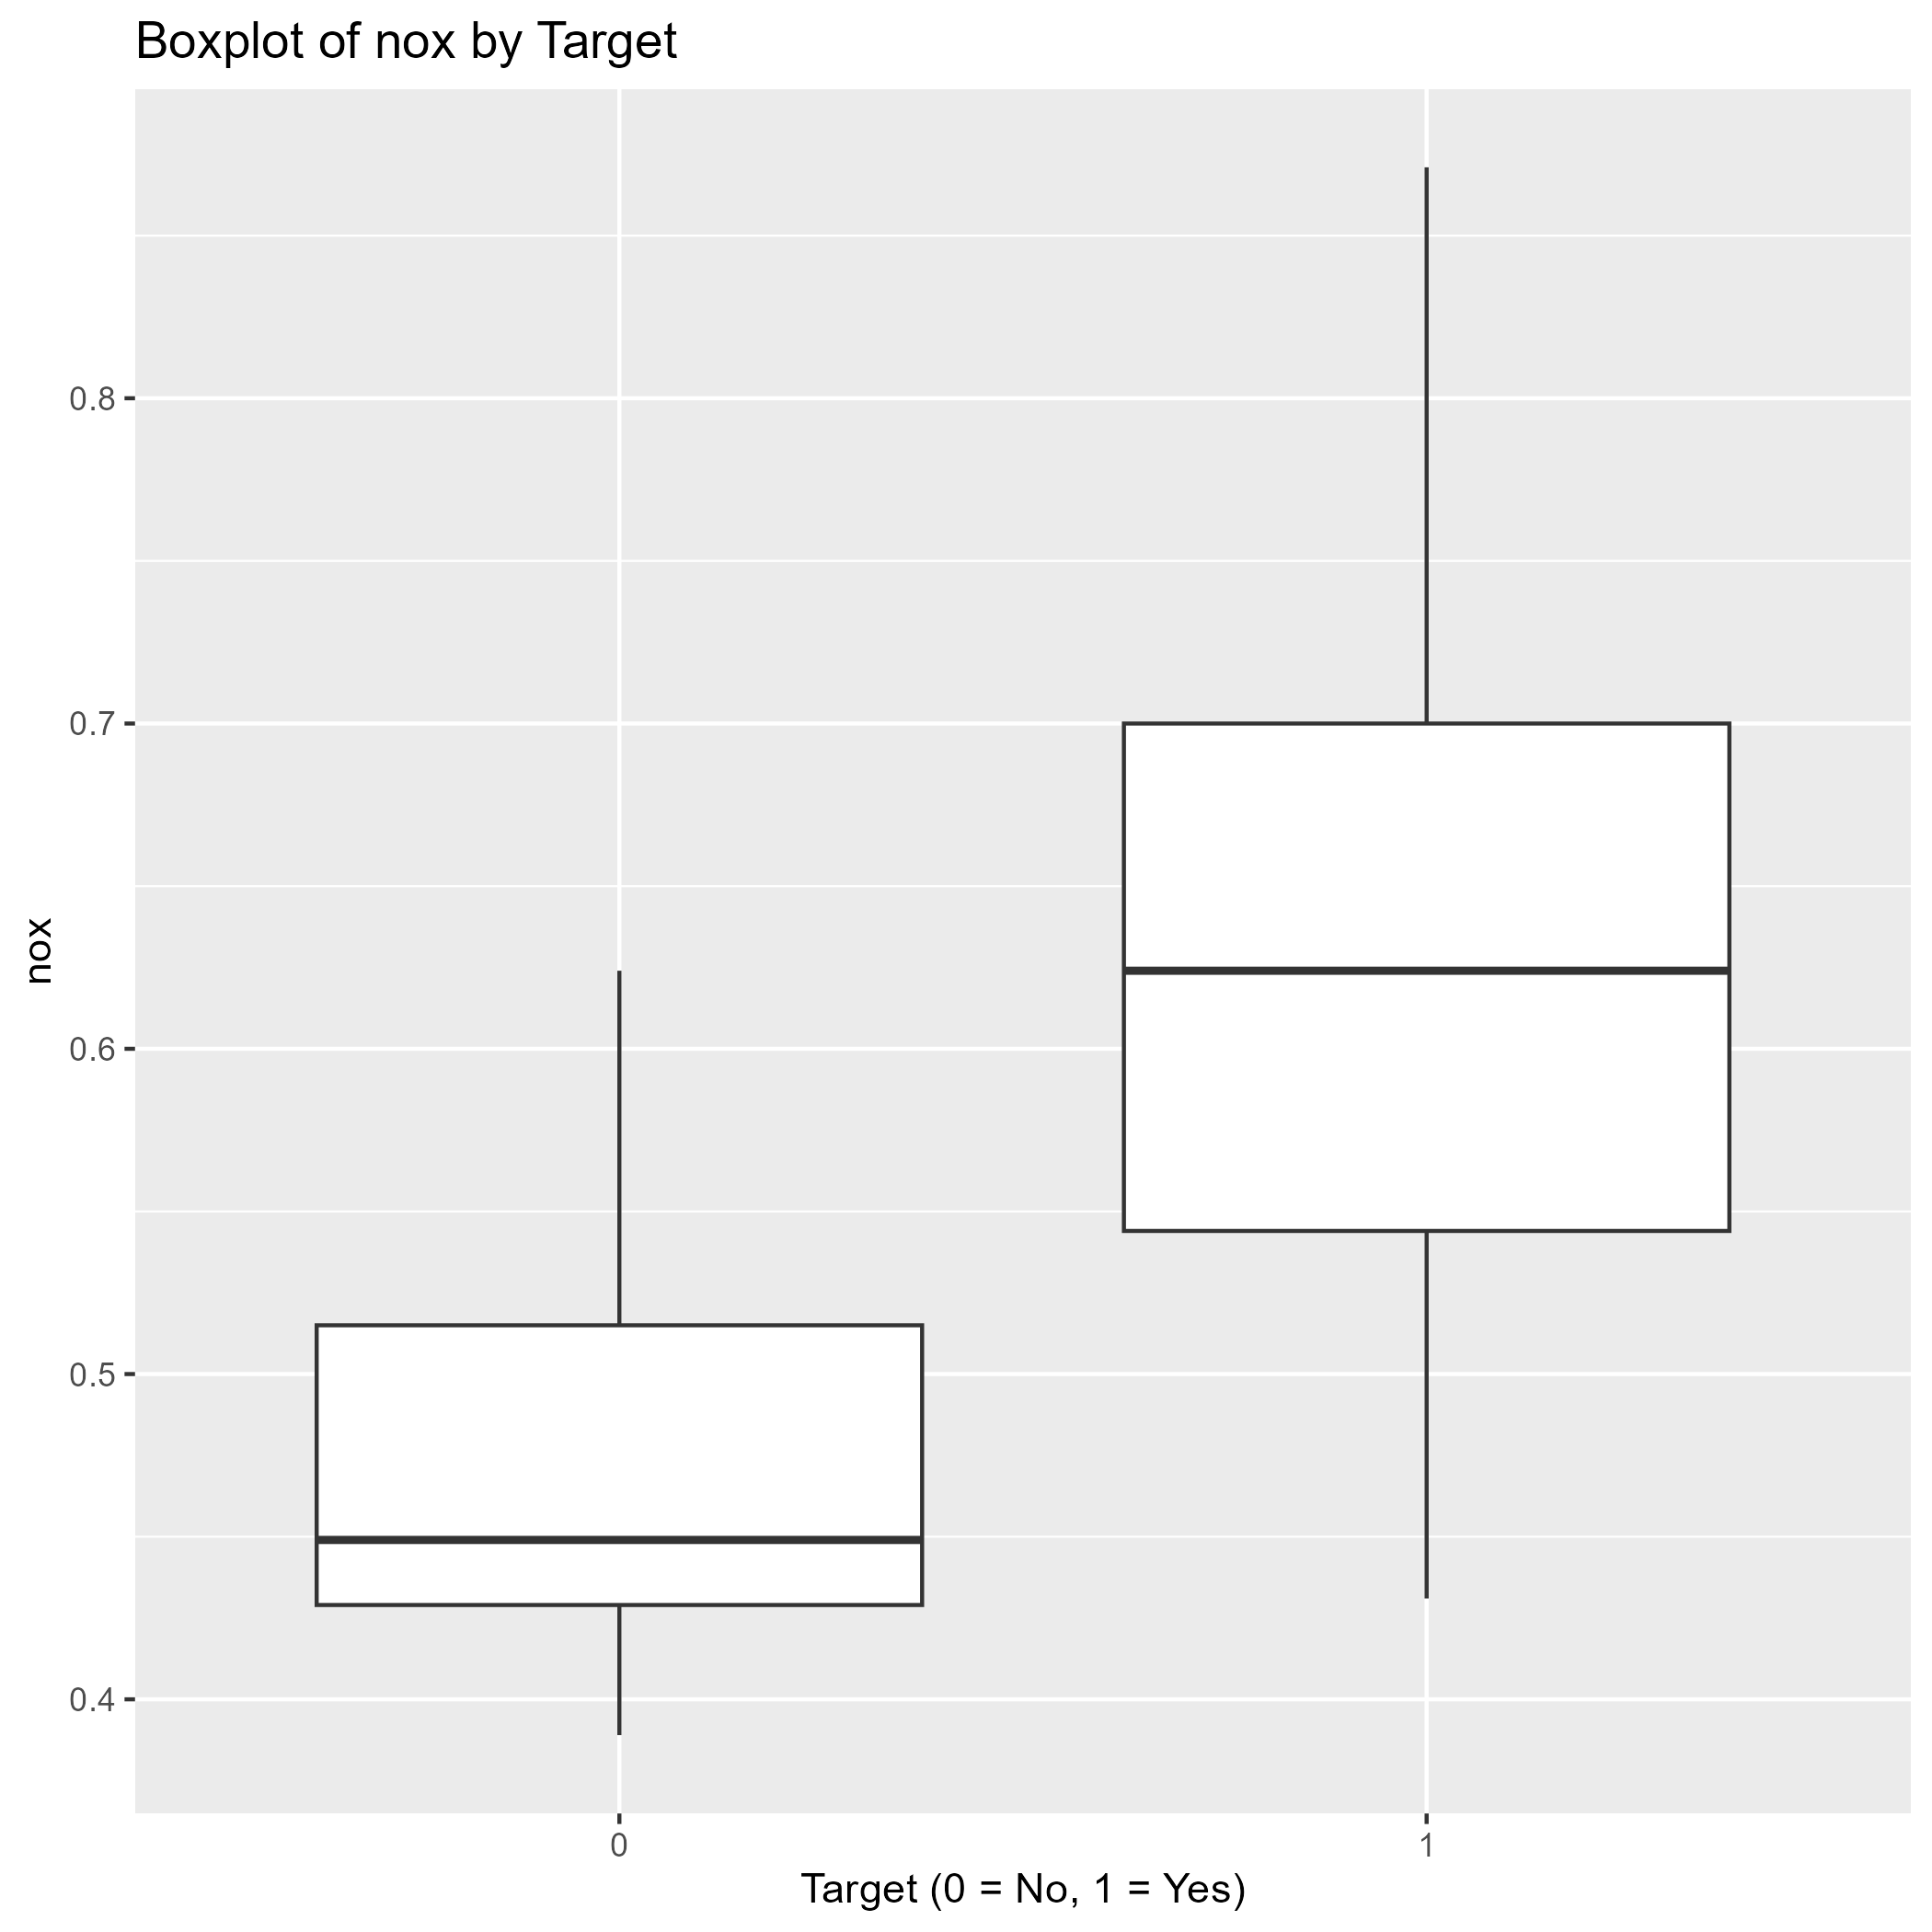
\includegraphics[keepaspectratio]{https://raw.githubusercontent.com/jhnboyy/CUNY_SPS_WORK/refs/heads/main/Spring2025/DATA621/DATA621_Homework3/images/Boxplotnox_plot.png}}
\pandocbounded{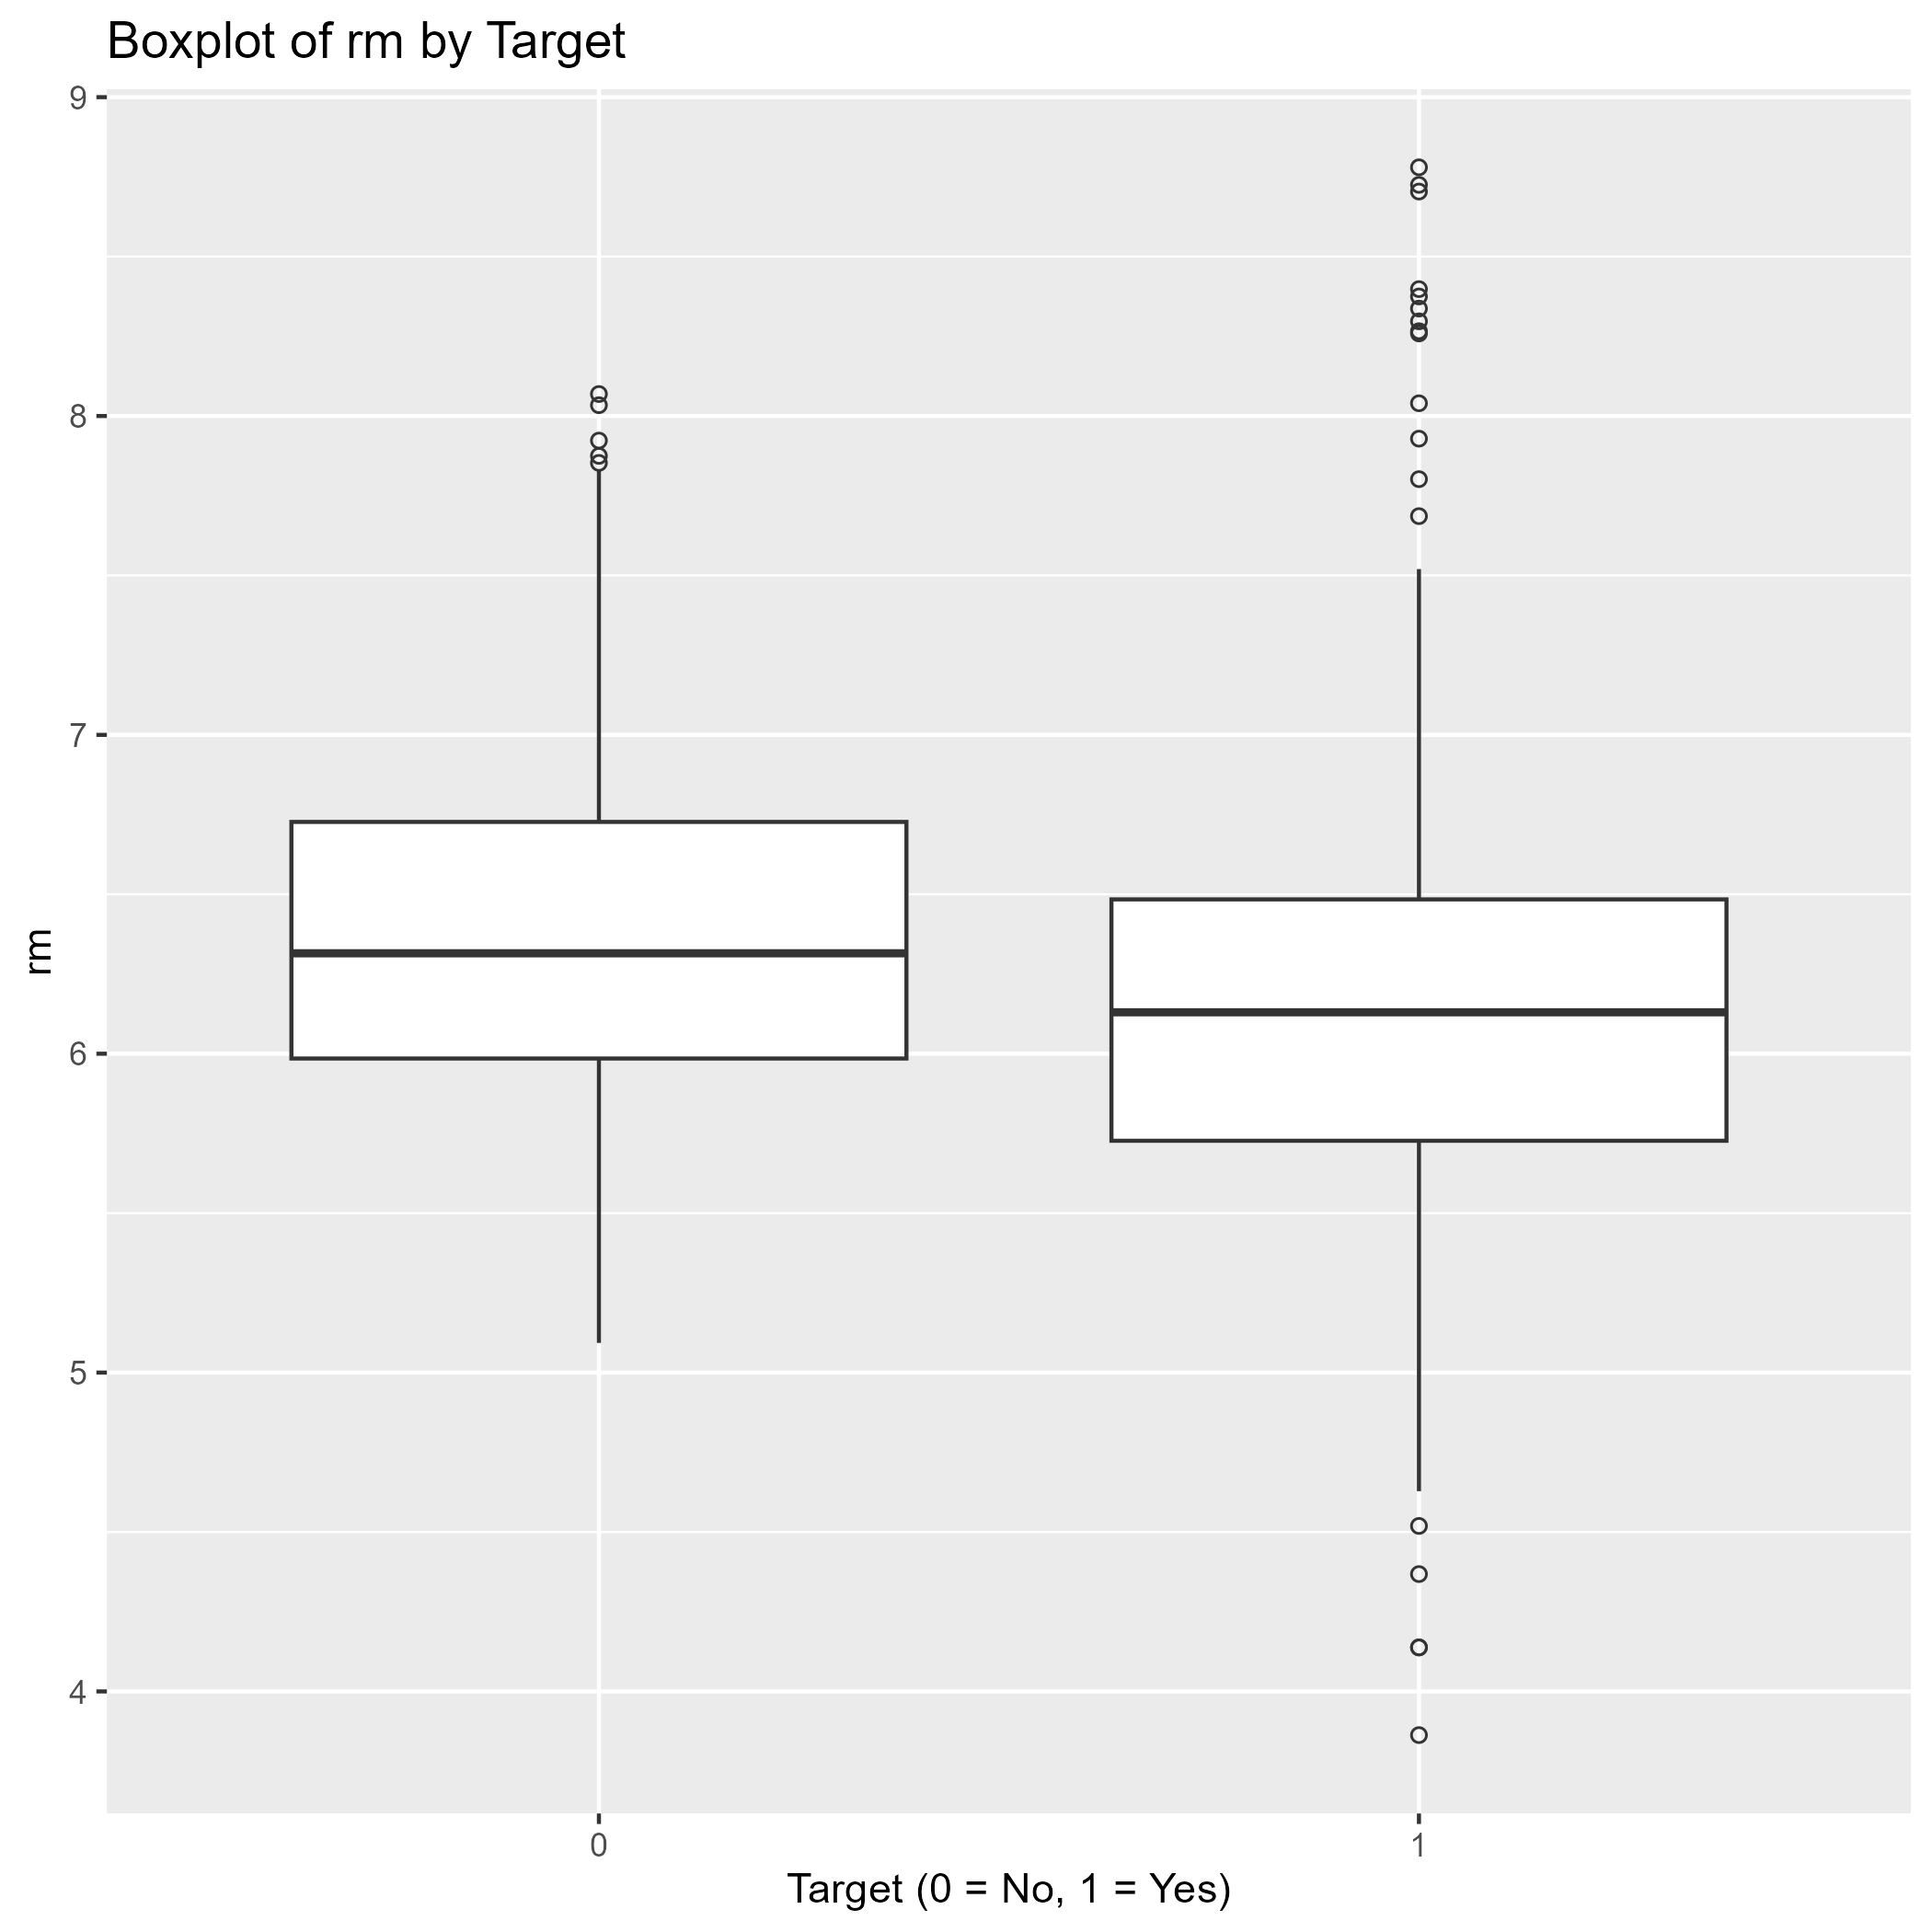
\includegraphics[keepaspectratio]{https://raw.githubusercontent.com/jhnboyy/CUNY_SPS_WORK/refs/heads/main/Spring2025/DATA621/DATA621_Homework3/images/Boxplotrm_plot.png}}
\pandocbounded{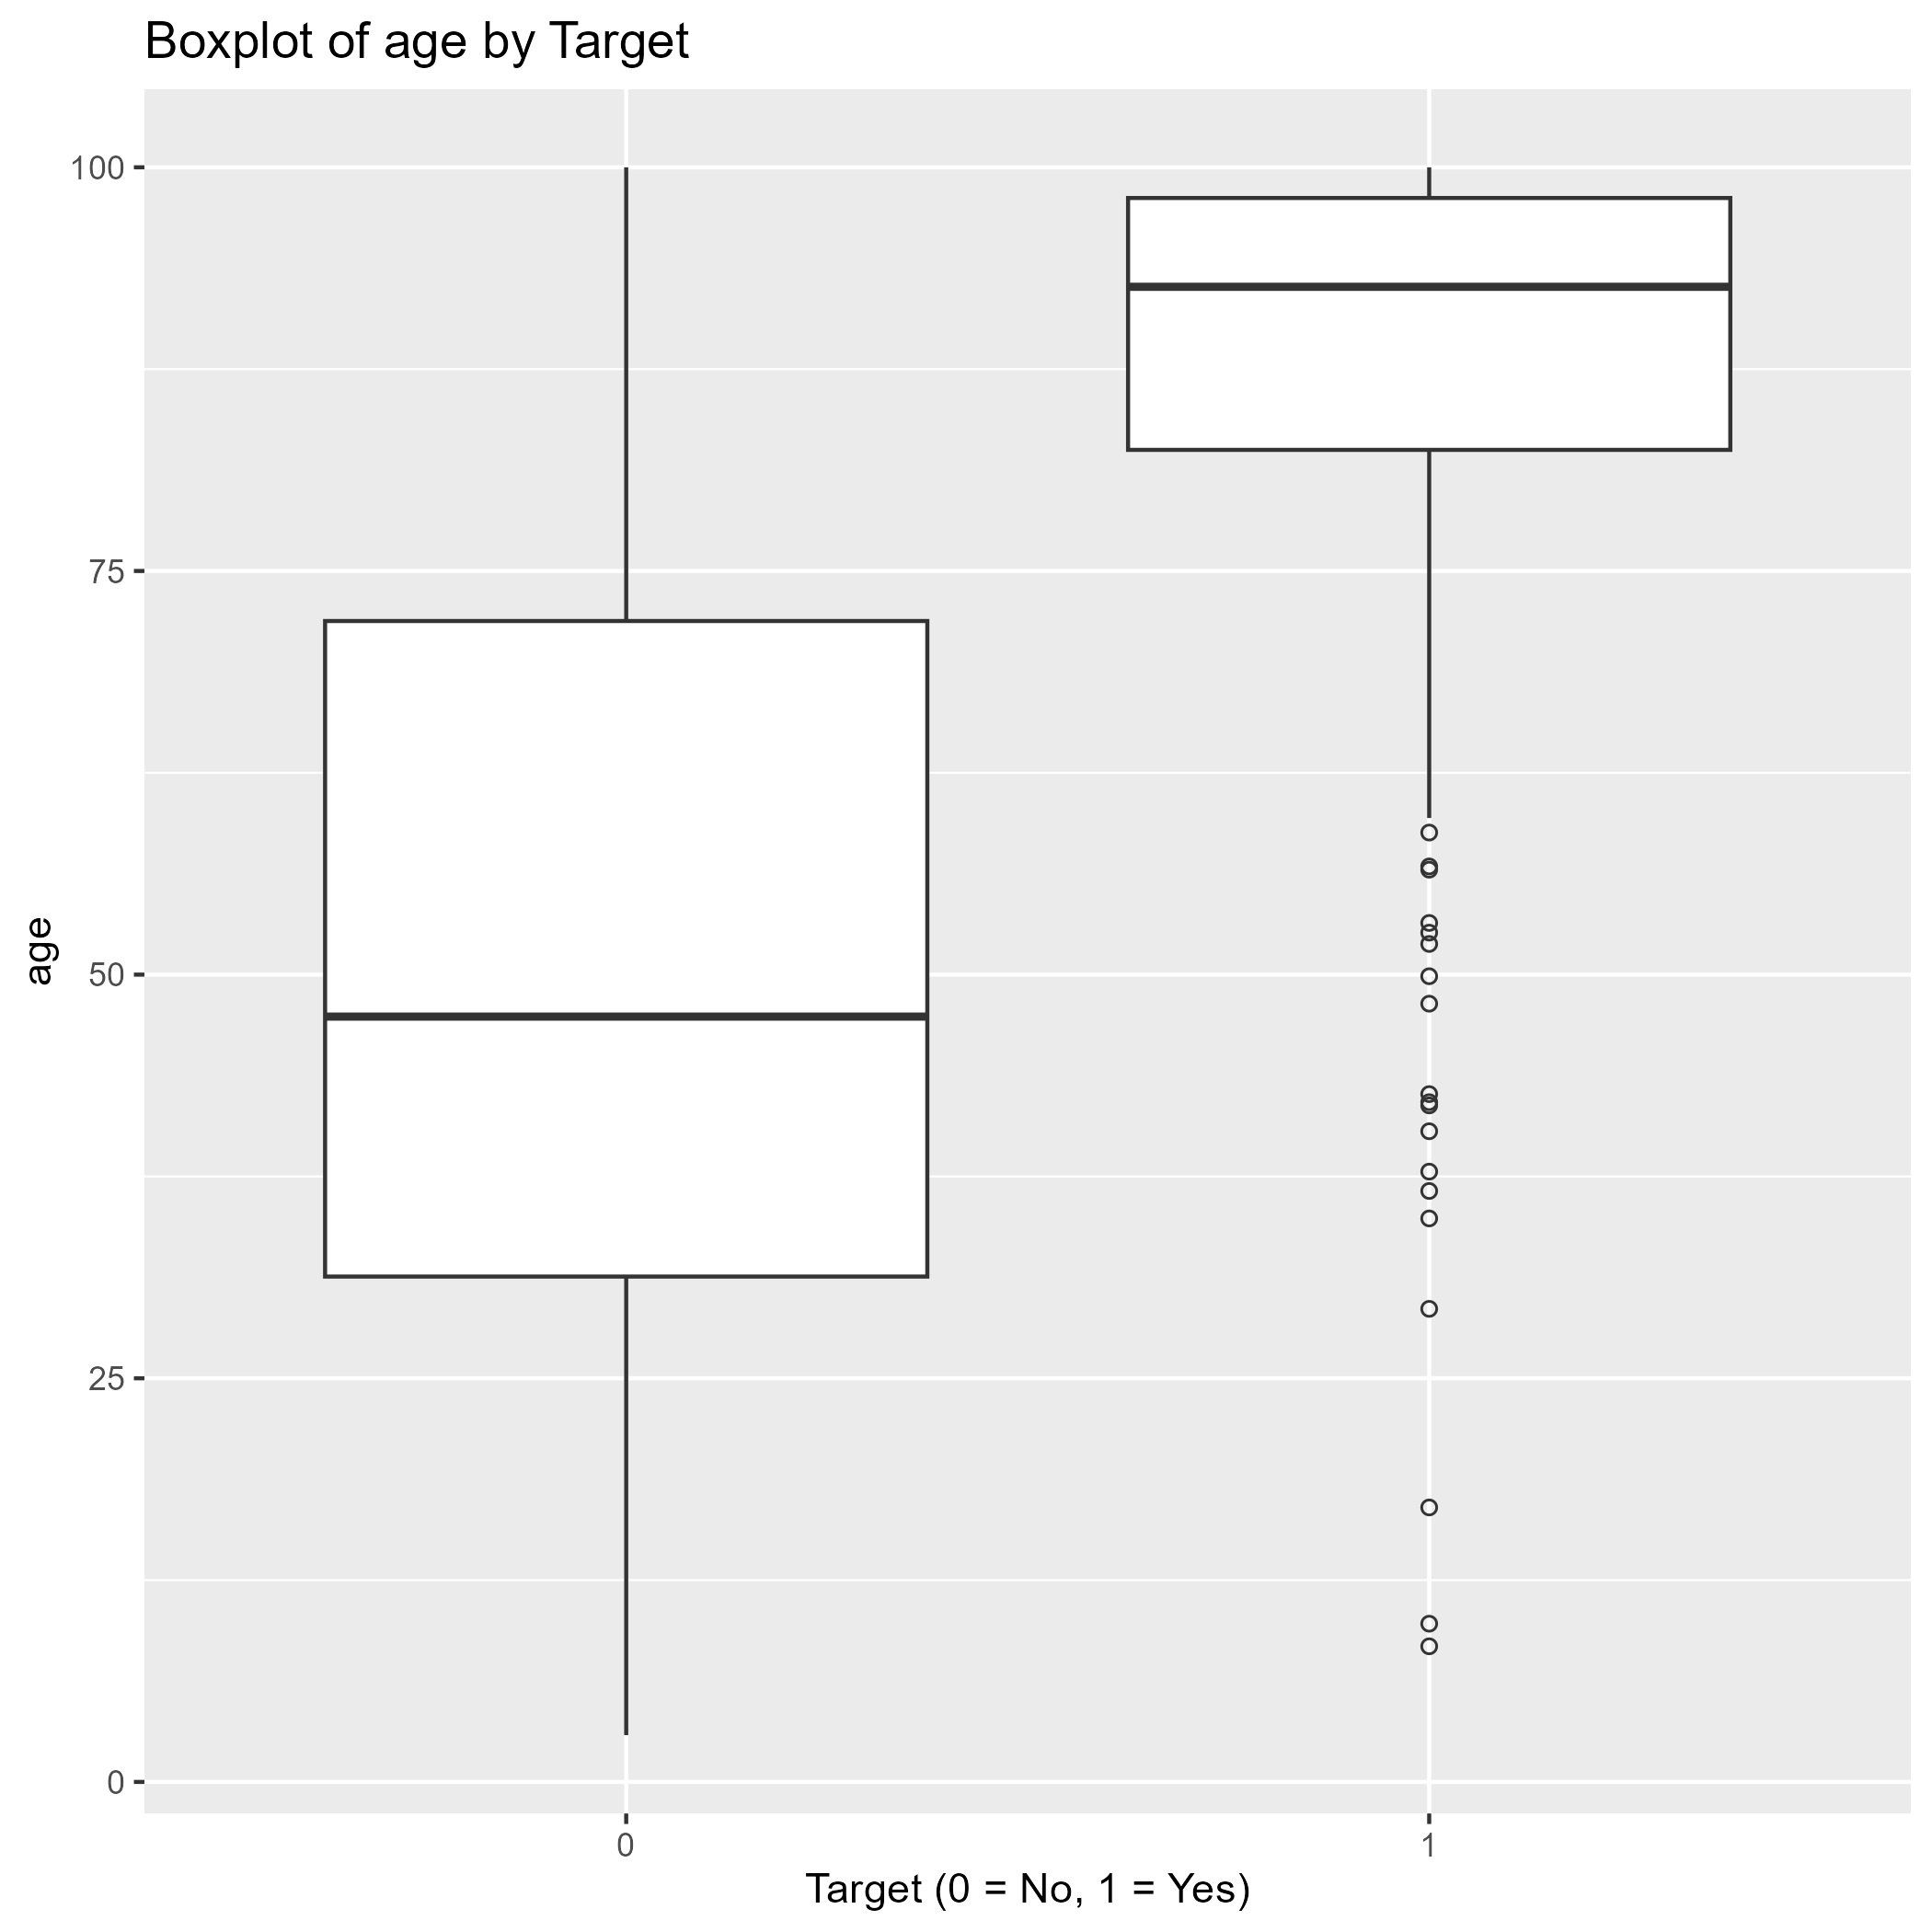
\includegraphics[keepaspectratio]{https://raw.githubusercontent.com/jhnboyy/CUNY_SPS_WORK/refs/heads/main/Spring2025/DATA621/DATA621_Homework3/images/Boxplotage_plot.png}}
\pandocbounded{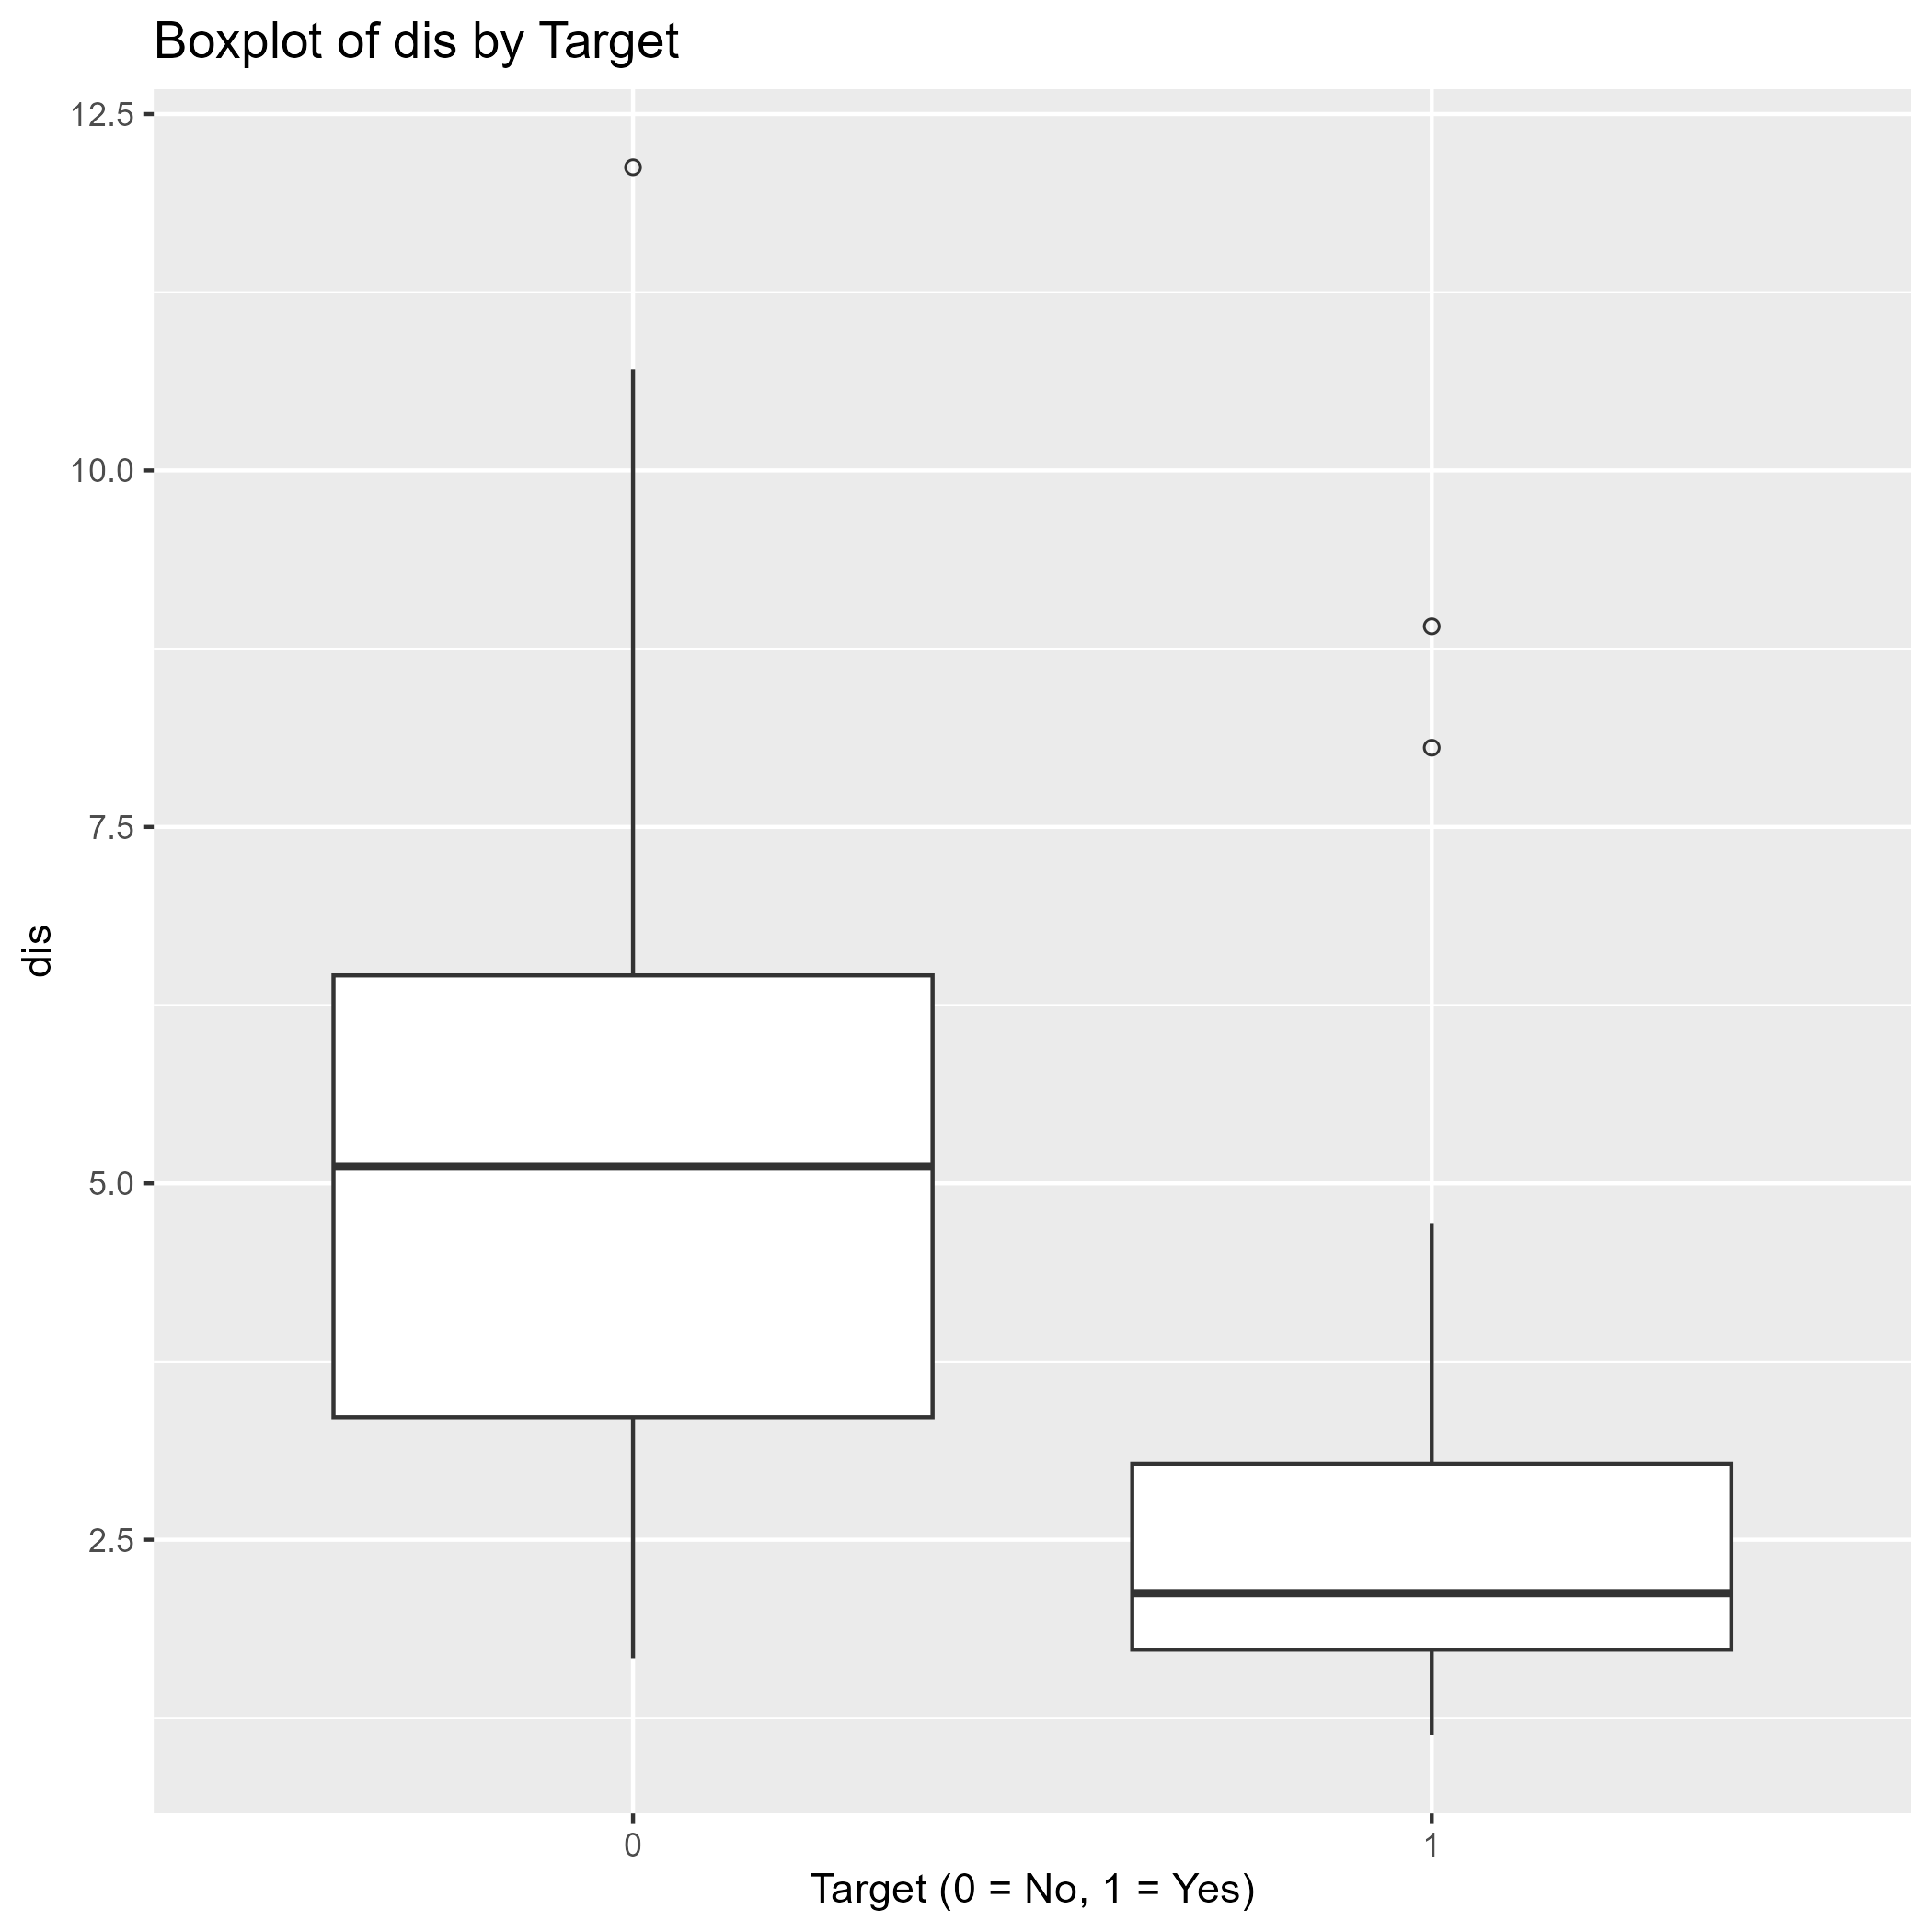
\includegraphics[keepaspectratio]{https://raw.githubusercontent.com/jhnboyy/CUNY_SPS_WORK/refs/heads/main/Spring2025/DATA621/DATA621_Homework3/images/Boxplotdis_plot.png}}
\pandocbounded{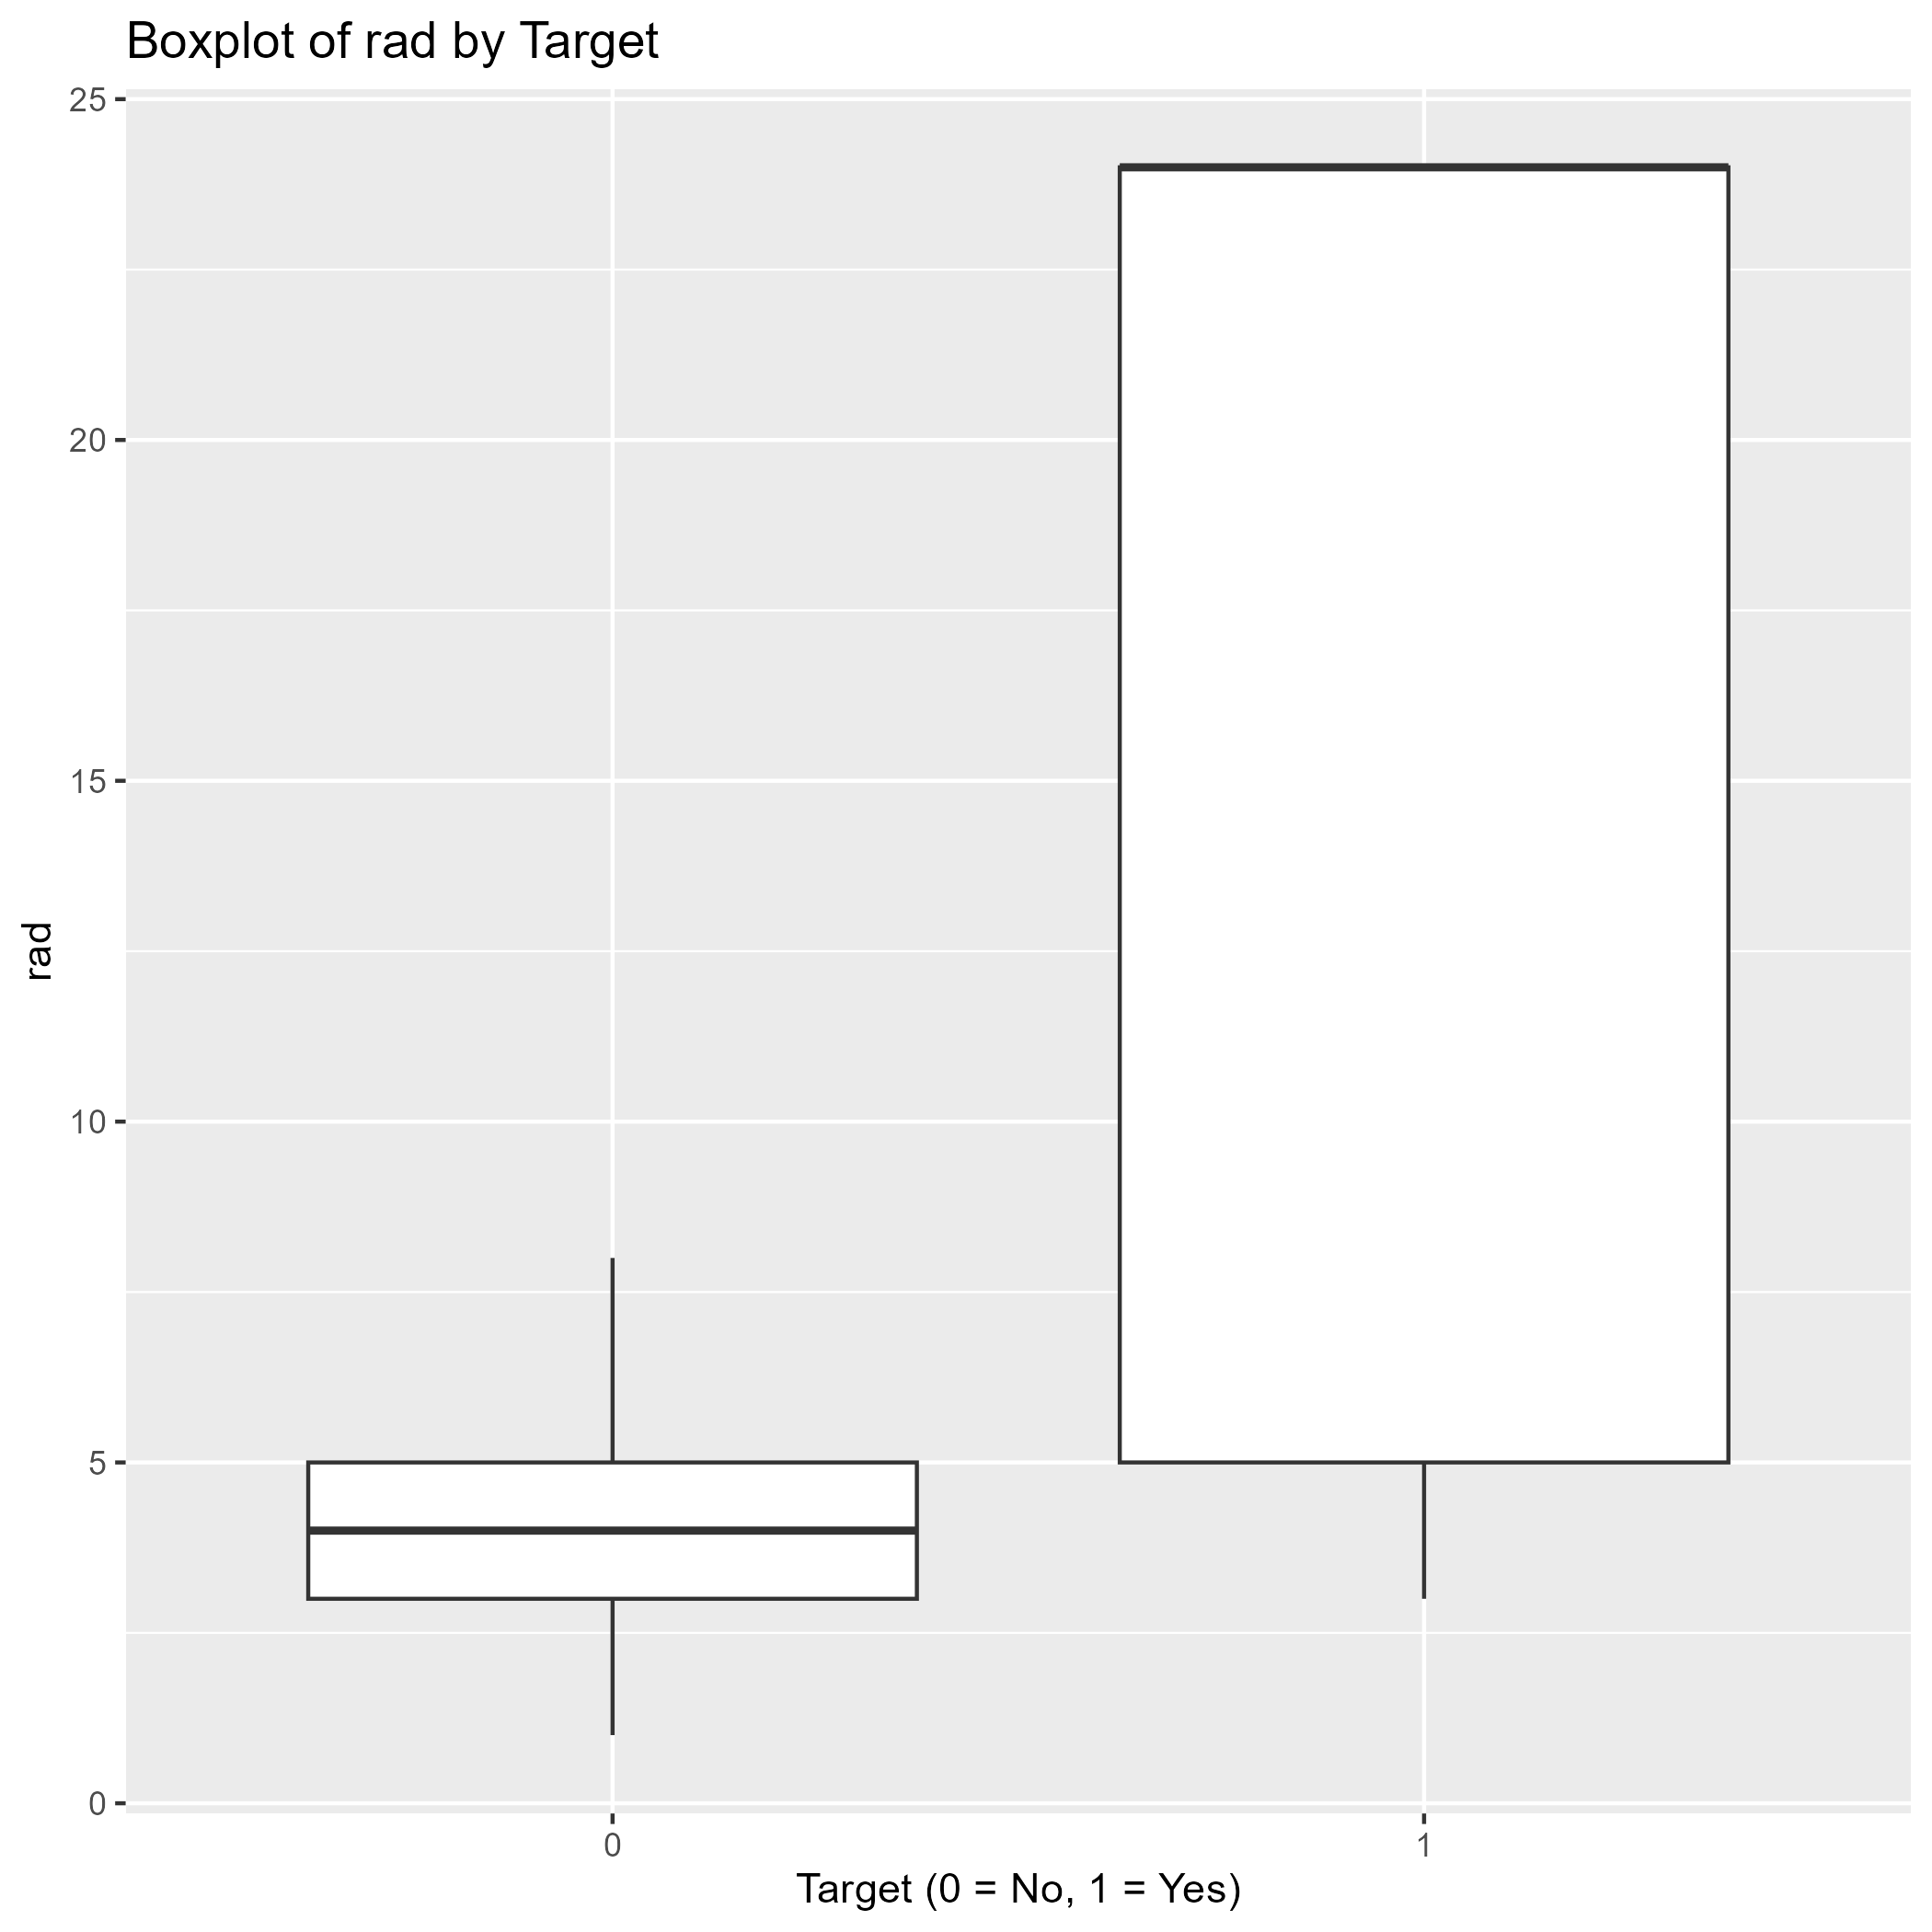
\includegraphics[keepaspectratio]{https://raw.githubusercontent.com/jhnboyy/CUNY_SPS_WORK/refs/heads/main/Spring2025/DATA621/DATA621_Homework3/images/Boxplotrad_plot.png}}
\pandocbounded{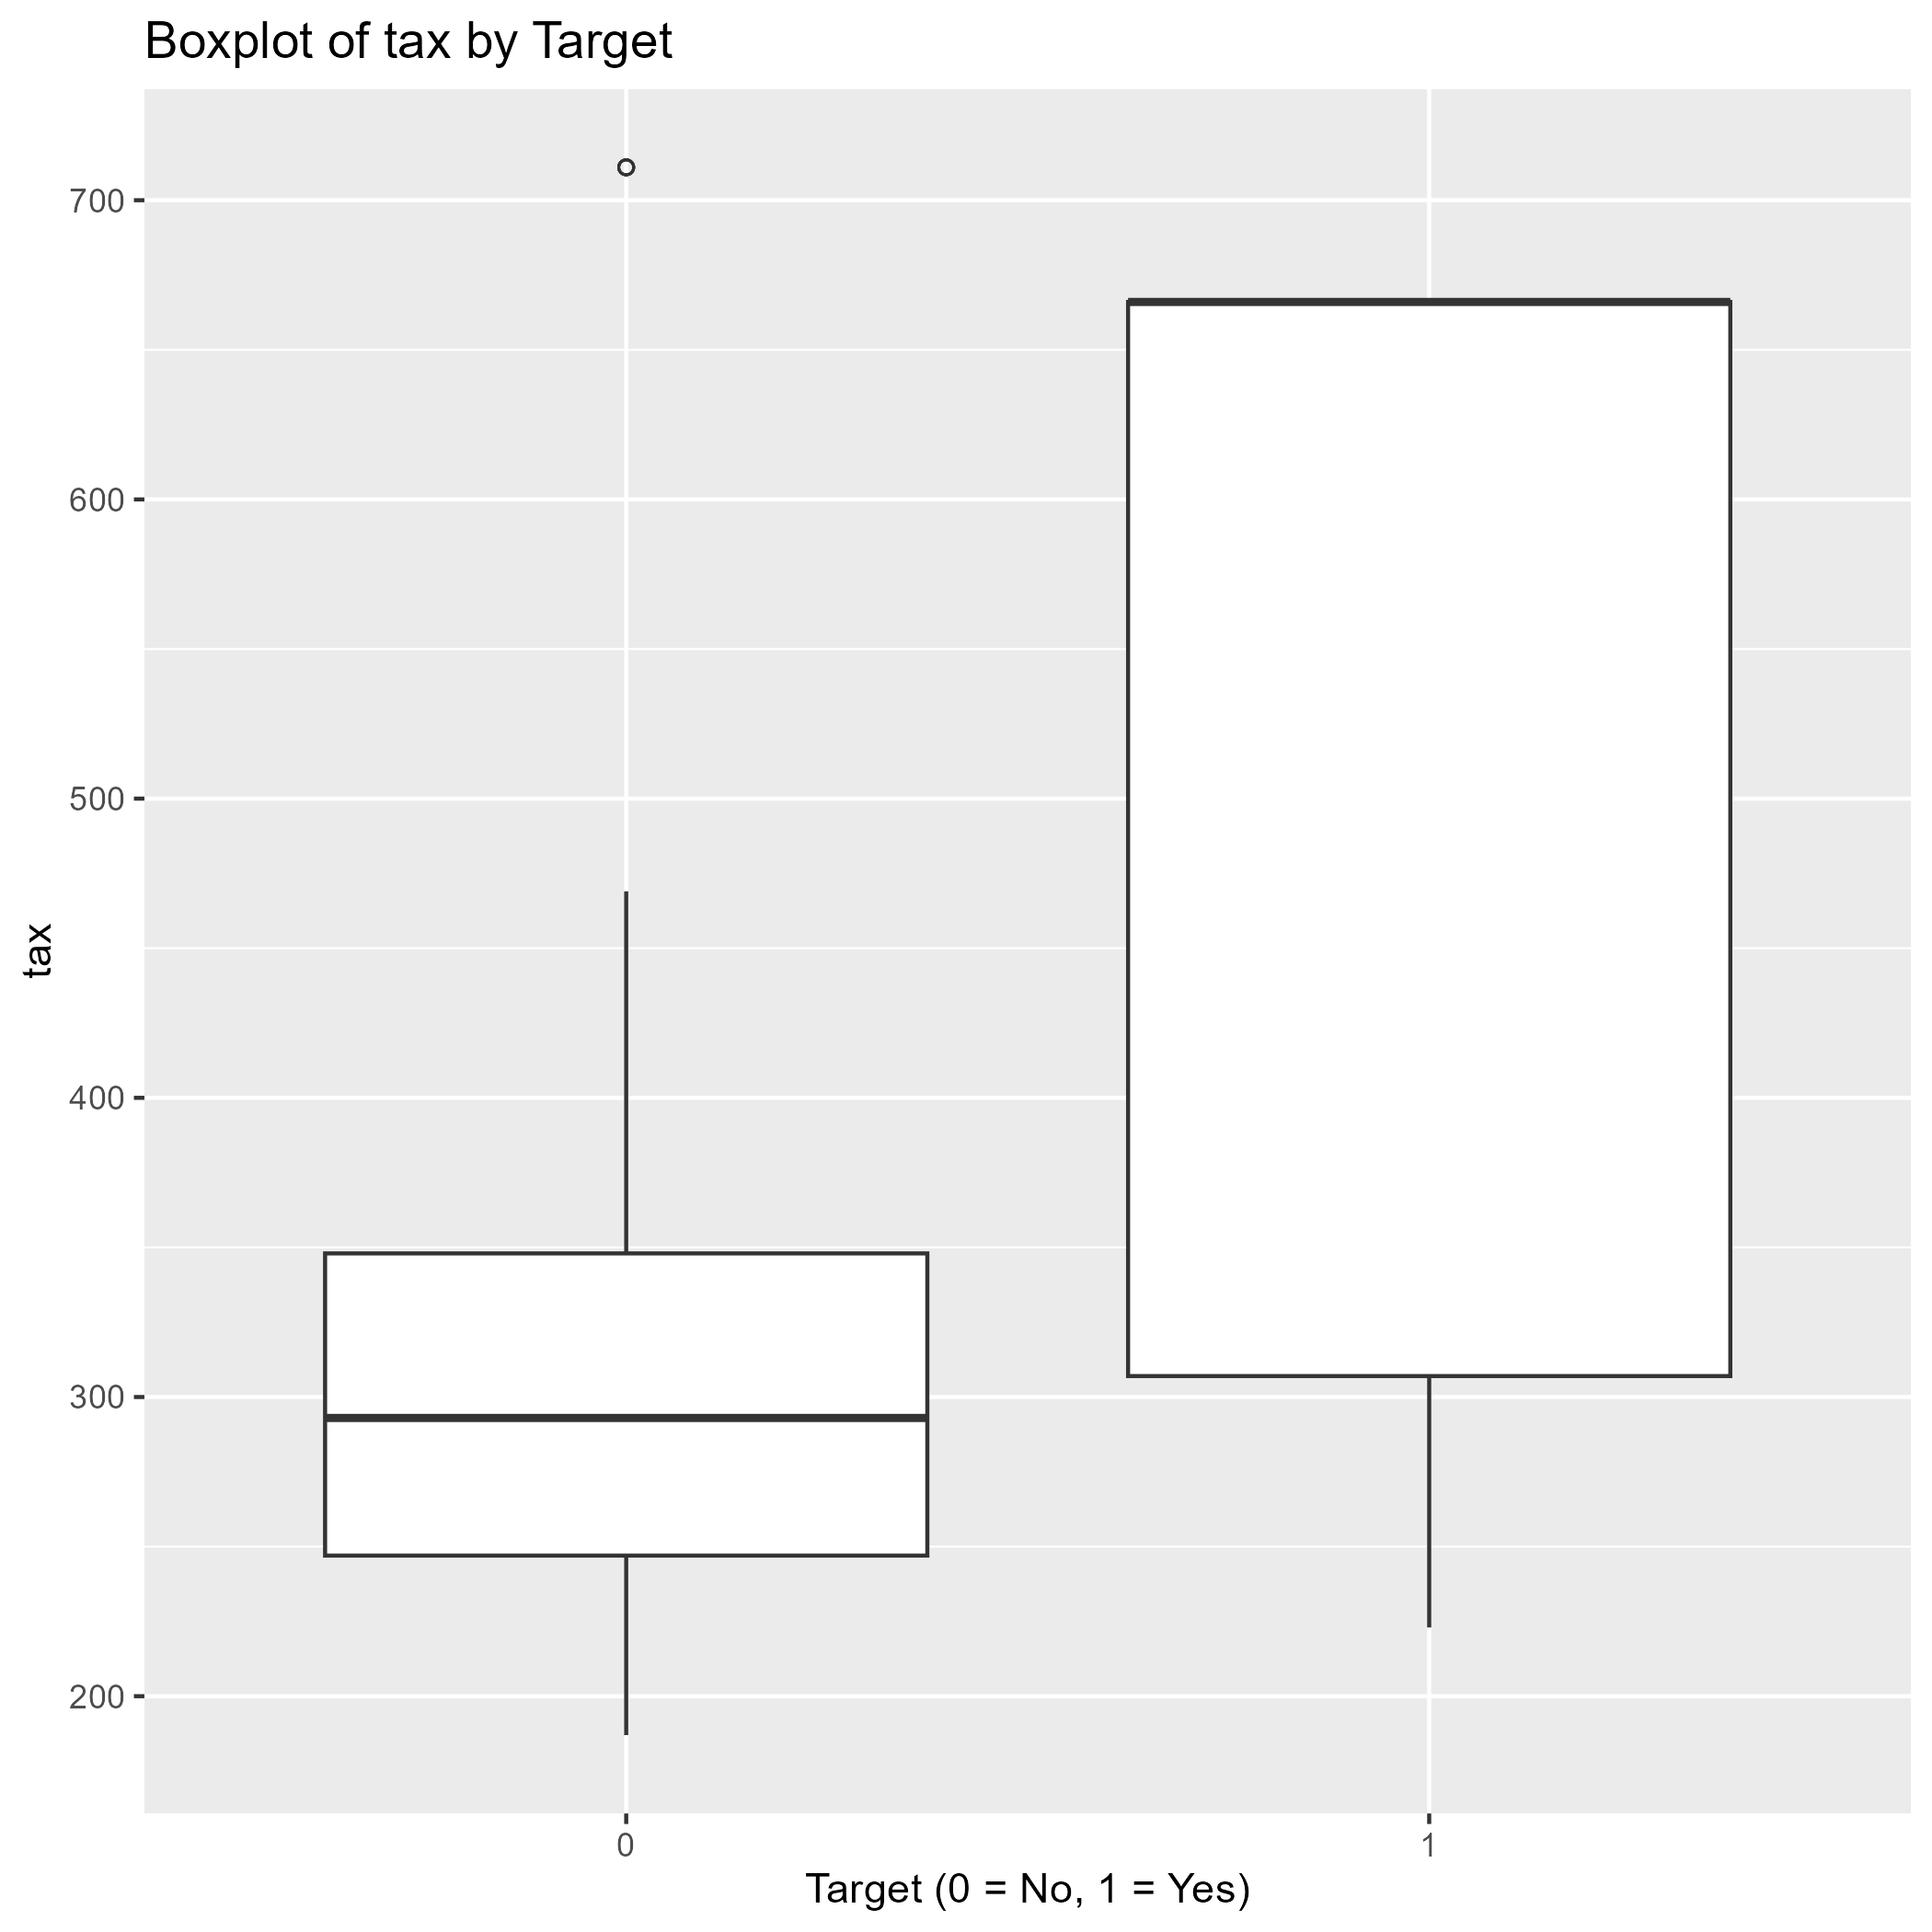
\includegraphics[keepaspectratio]{https://raw.githubusercontent.com/jhnboyy/CUNY_SPS_WORK/refs/heads/main/Spring2025/DATA621/DATA621_Homework3/images/Boxplottax_plot.png}}
\pandocbounded{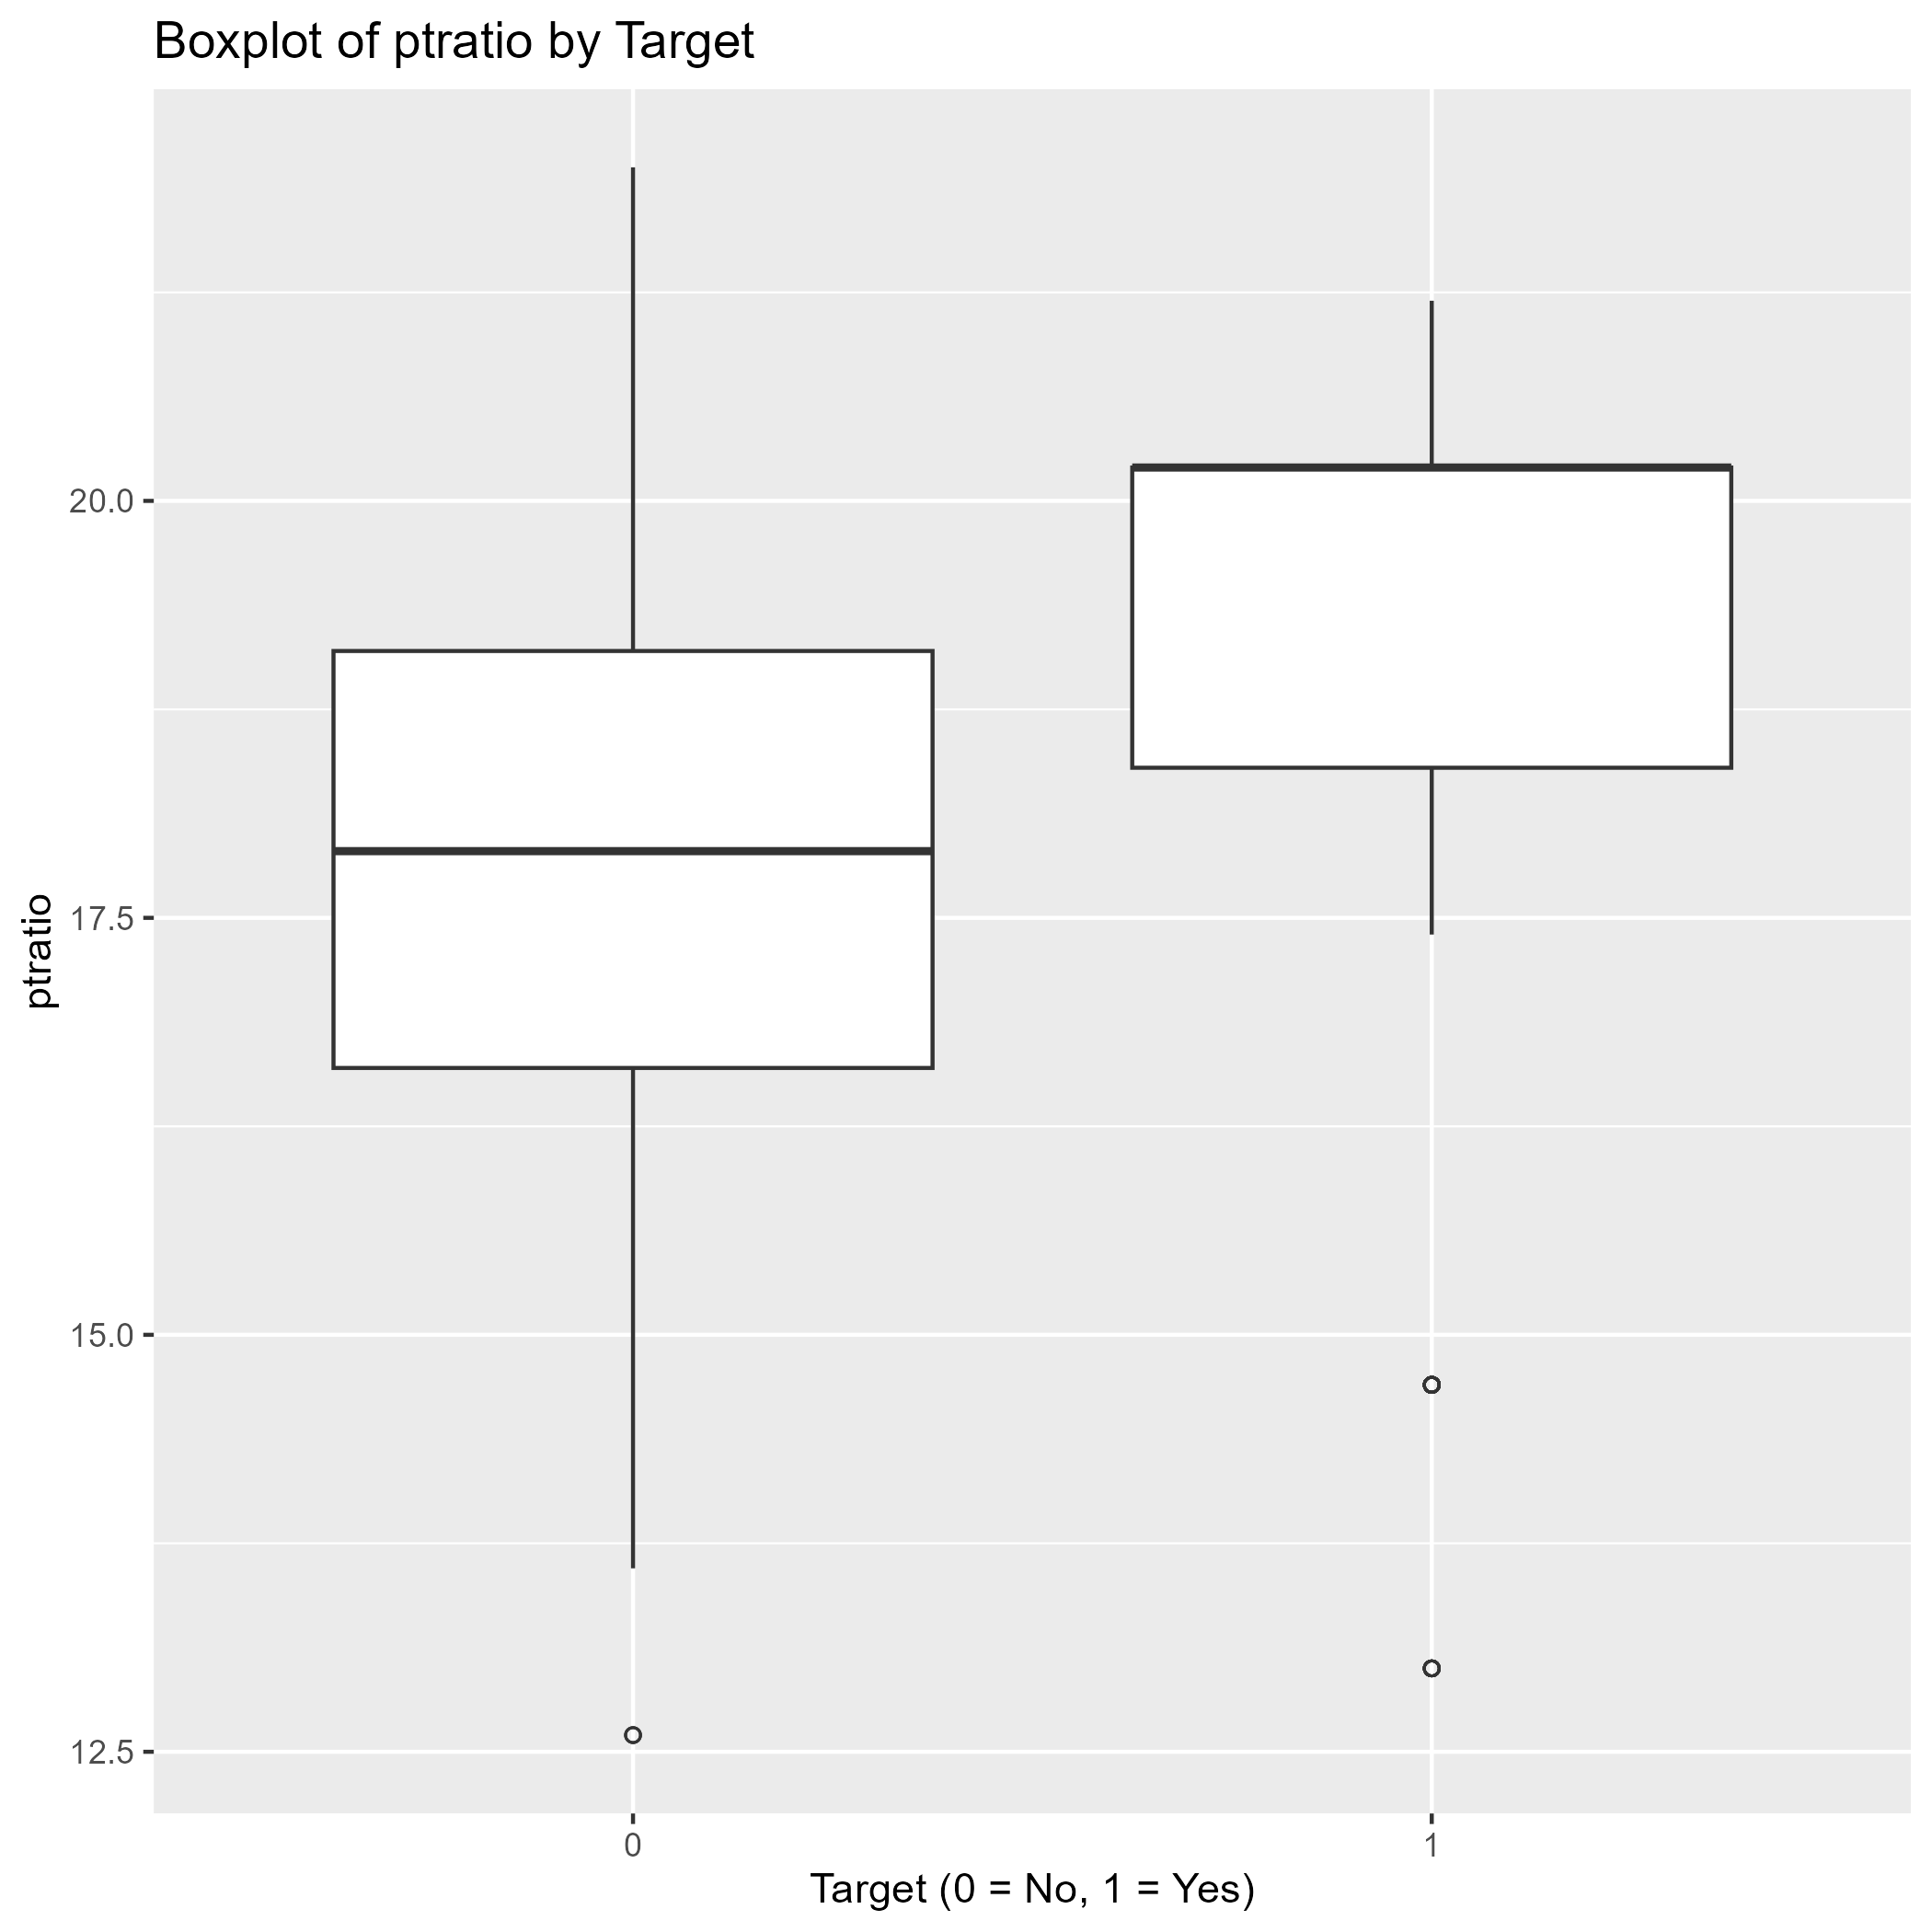
\includegraphics[keepaspectratio]{https://raw.githubusercontent.com/jhnboyy/CUNY_SPS_WORK/refs/heads/main/Spring2025/DATA621/DATA621_Homework3/images/Boxplotptratio_plot.png}}
\pandocbounded{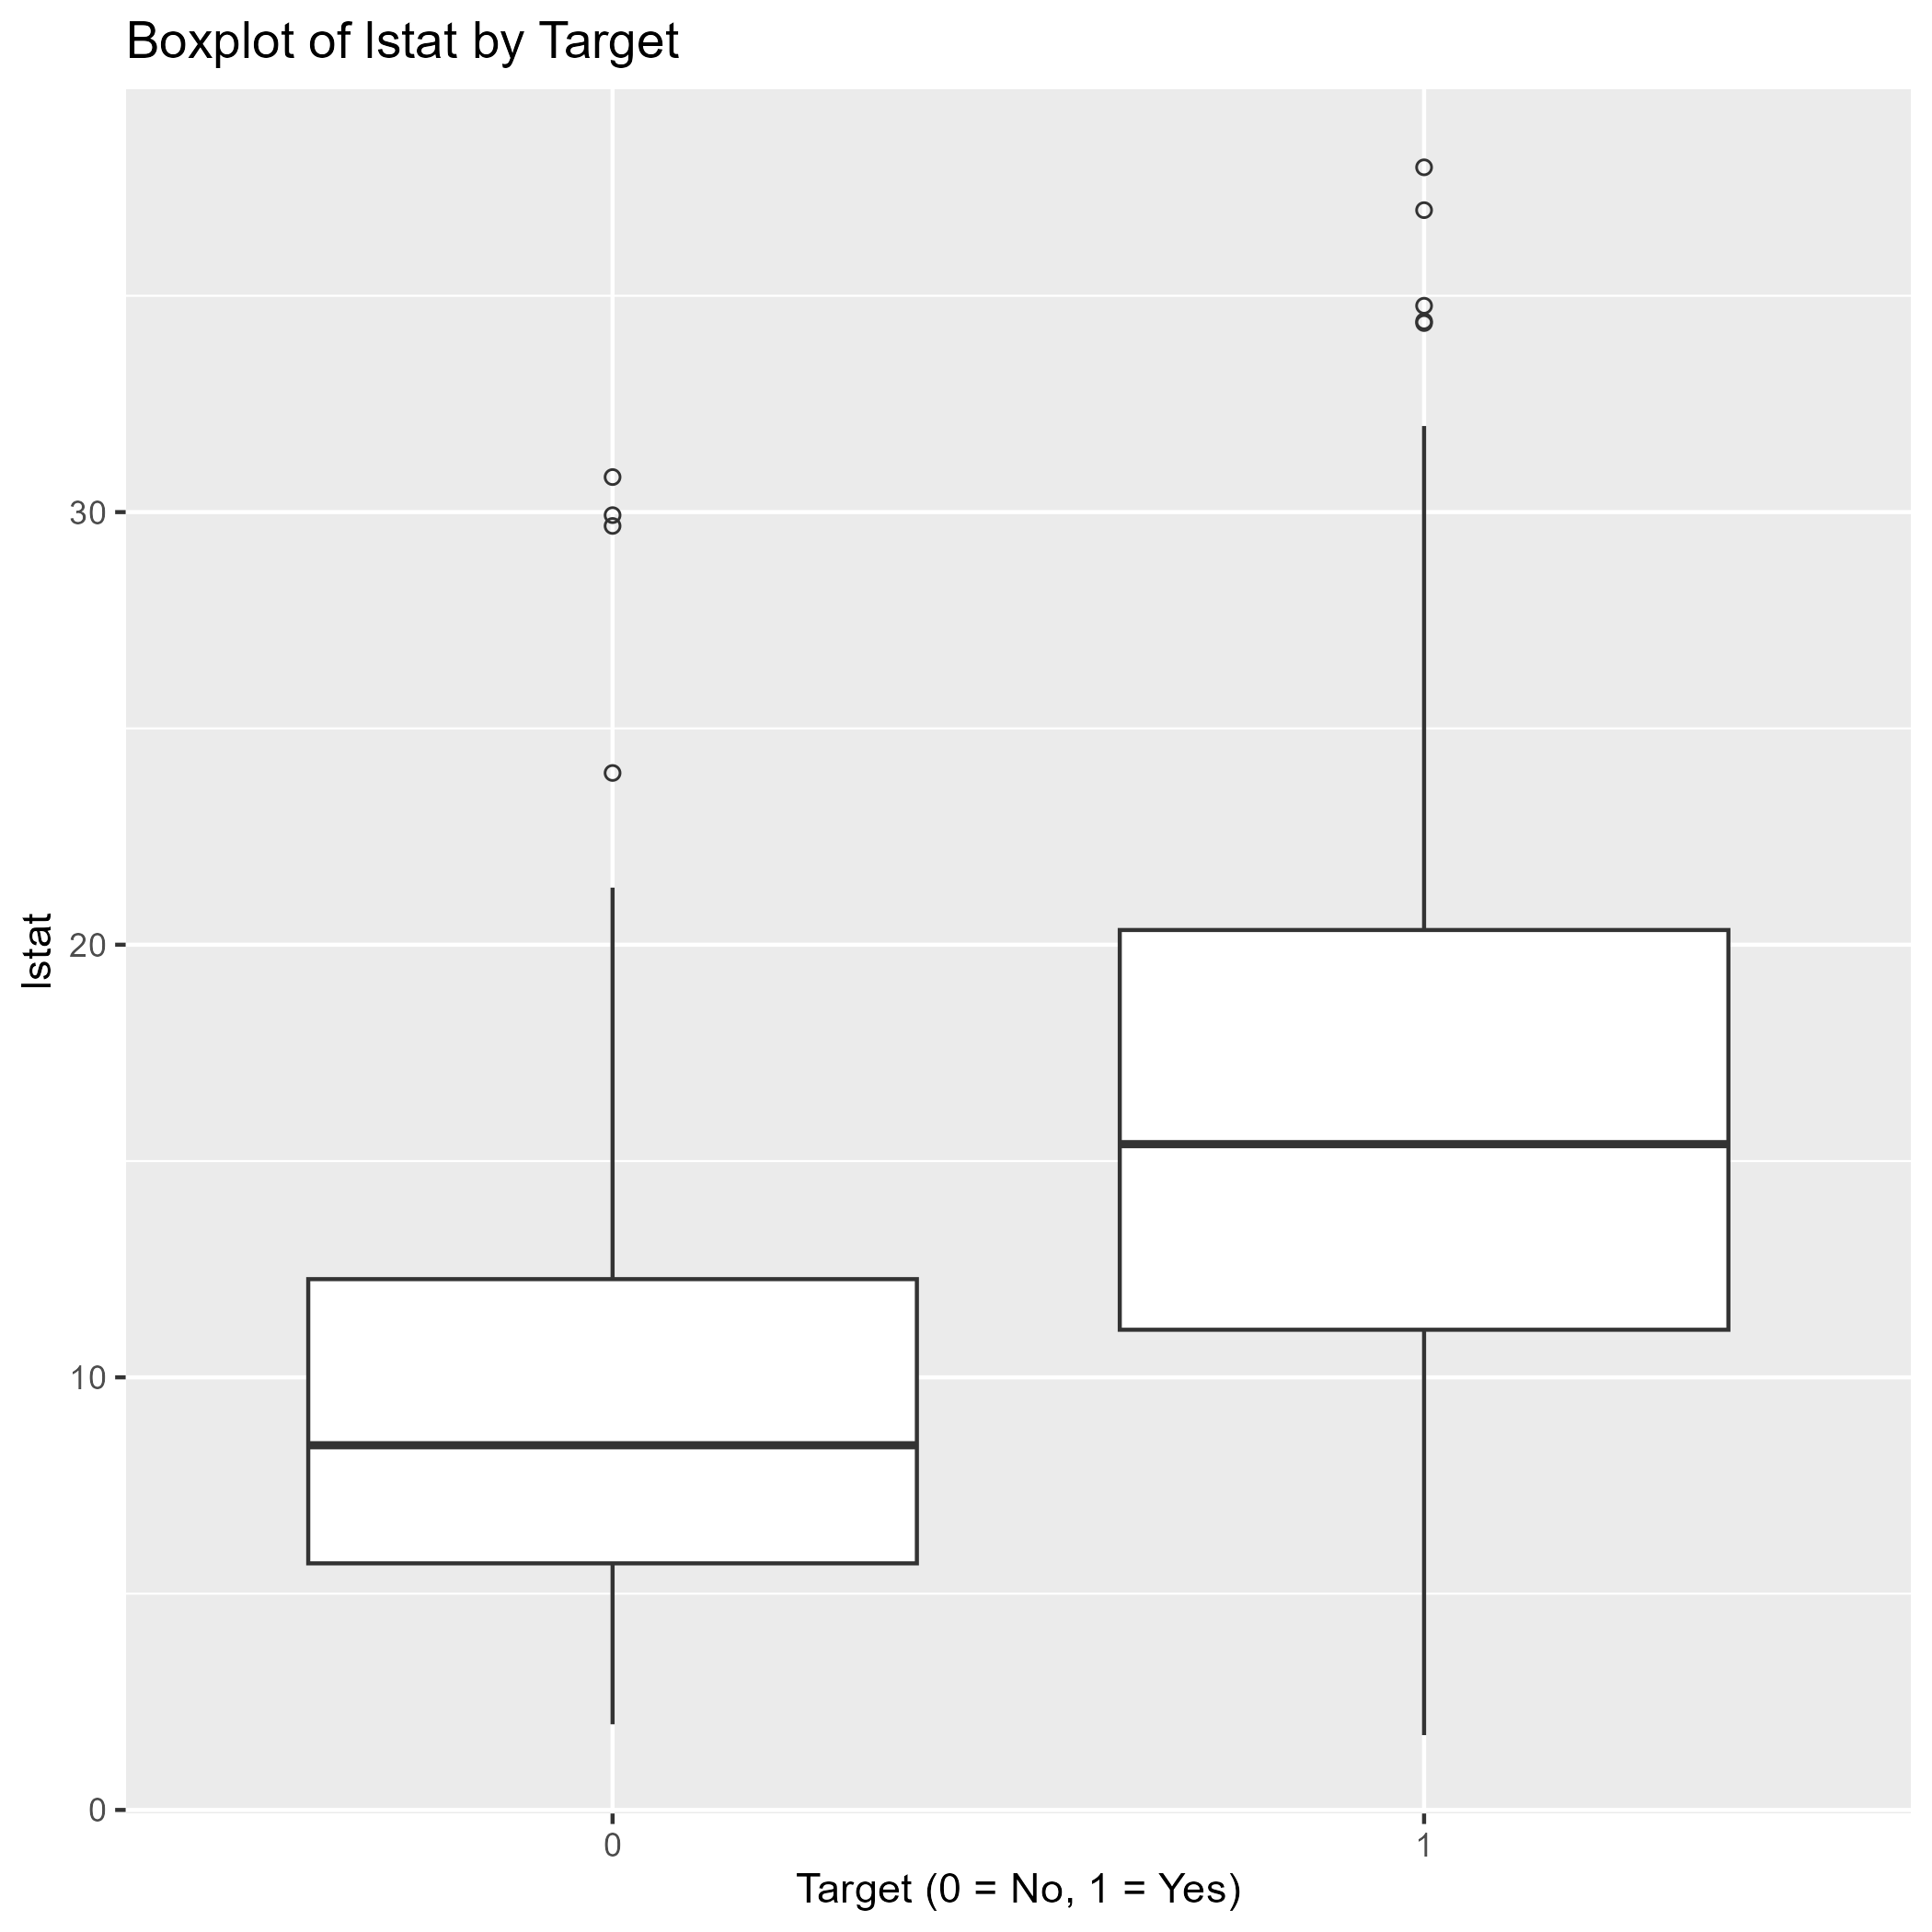
\includegraphics[keepaspectratio]{https://raw.githubusercontent.com/jhnboyy/CUNY_SPS_WORK/refs/heads/main/Spring2025/DATA621/DATA621_Homework3/images/Boxplotlstat_plot.png}}
\pandocbounded{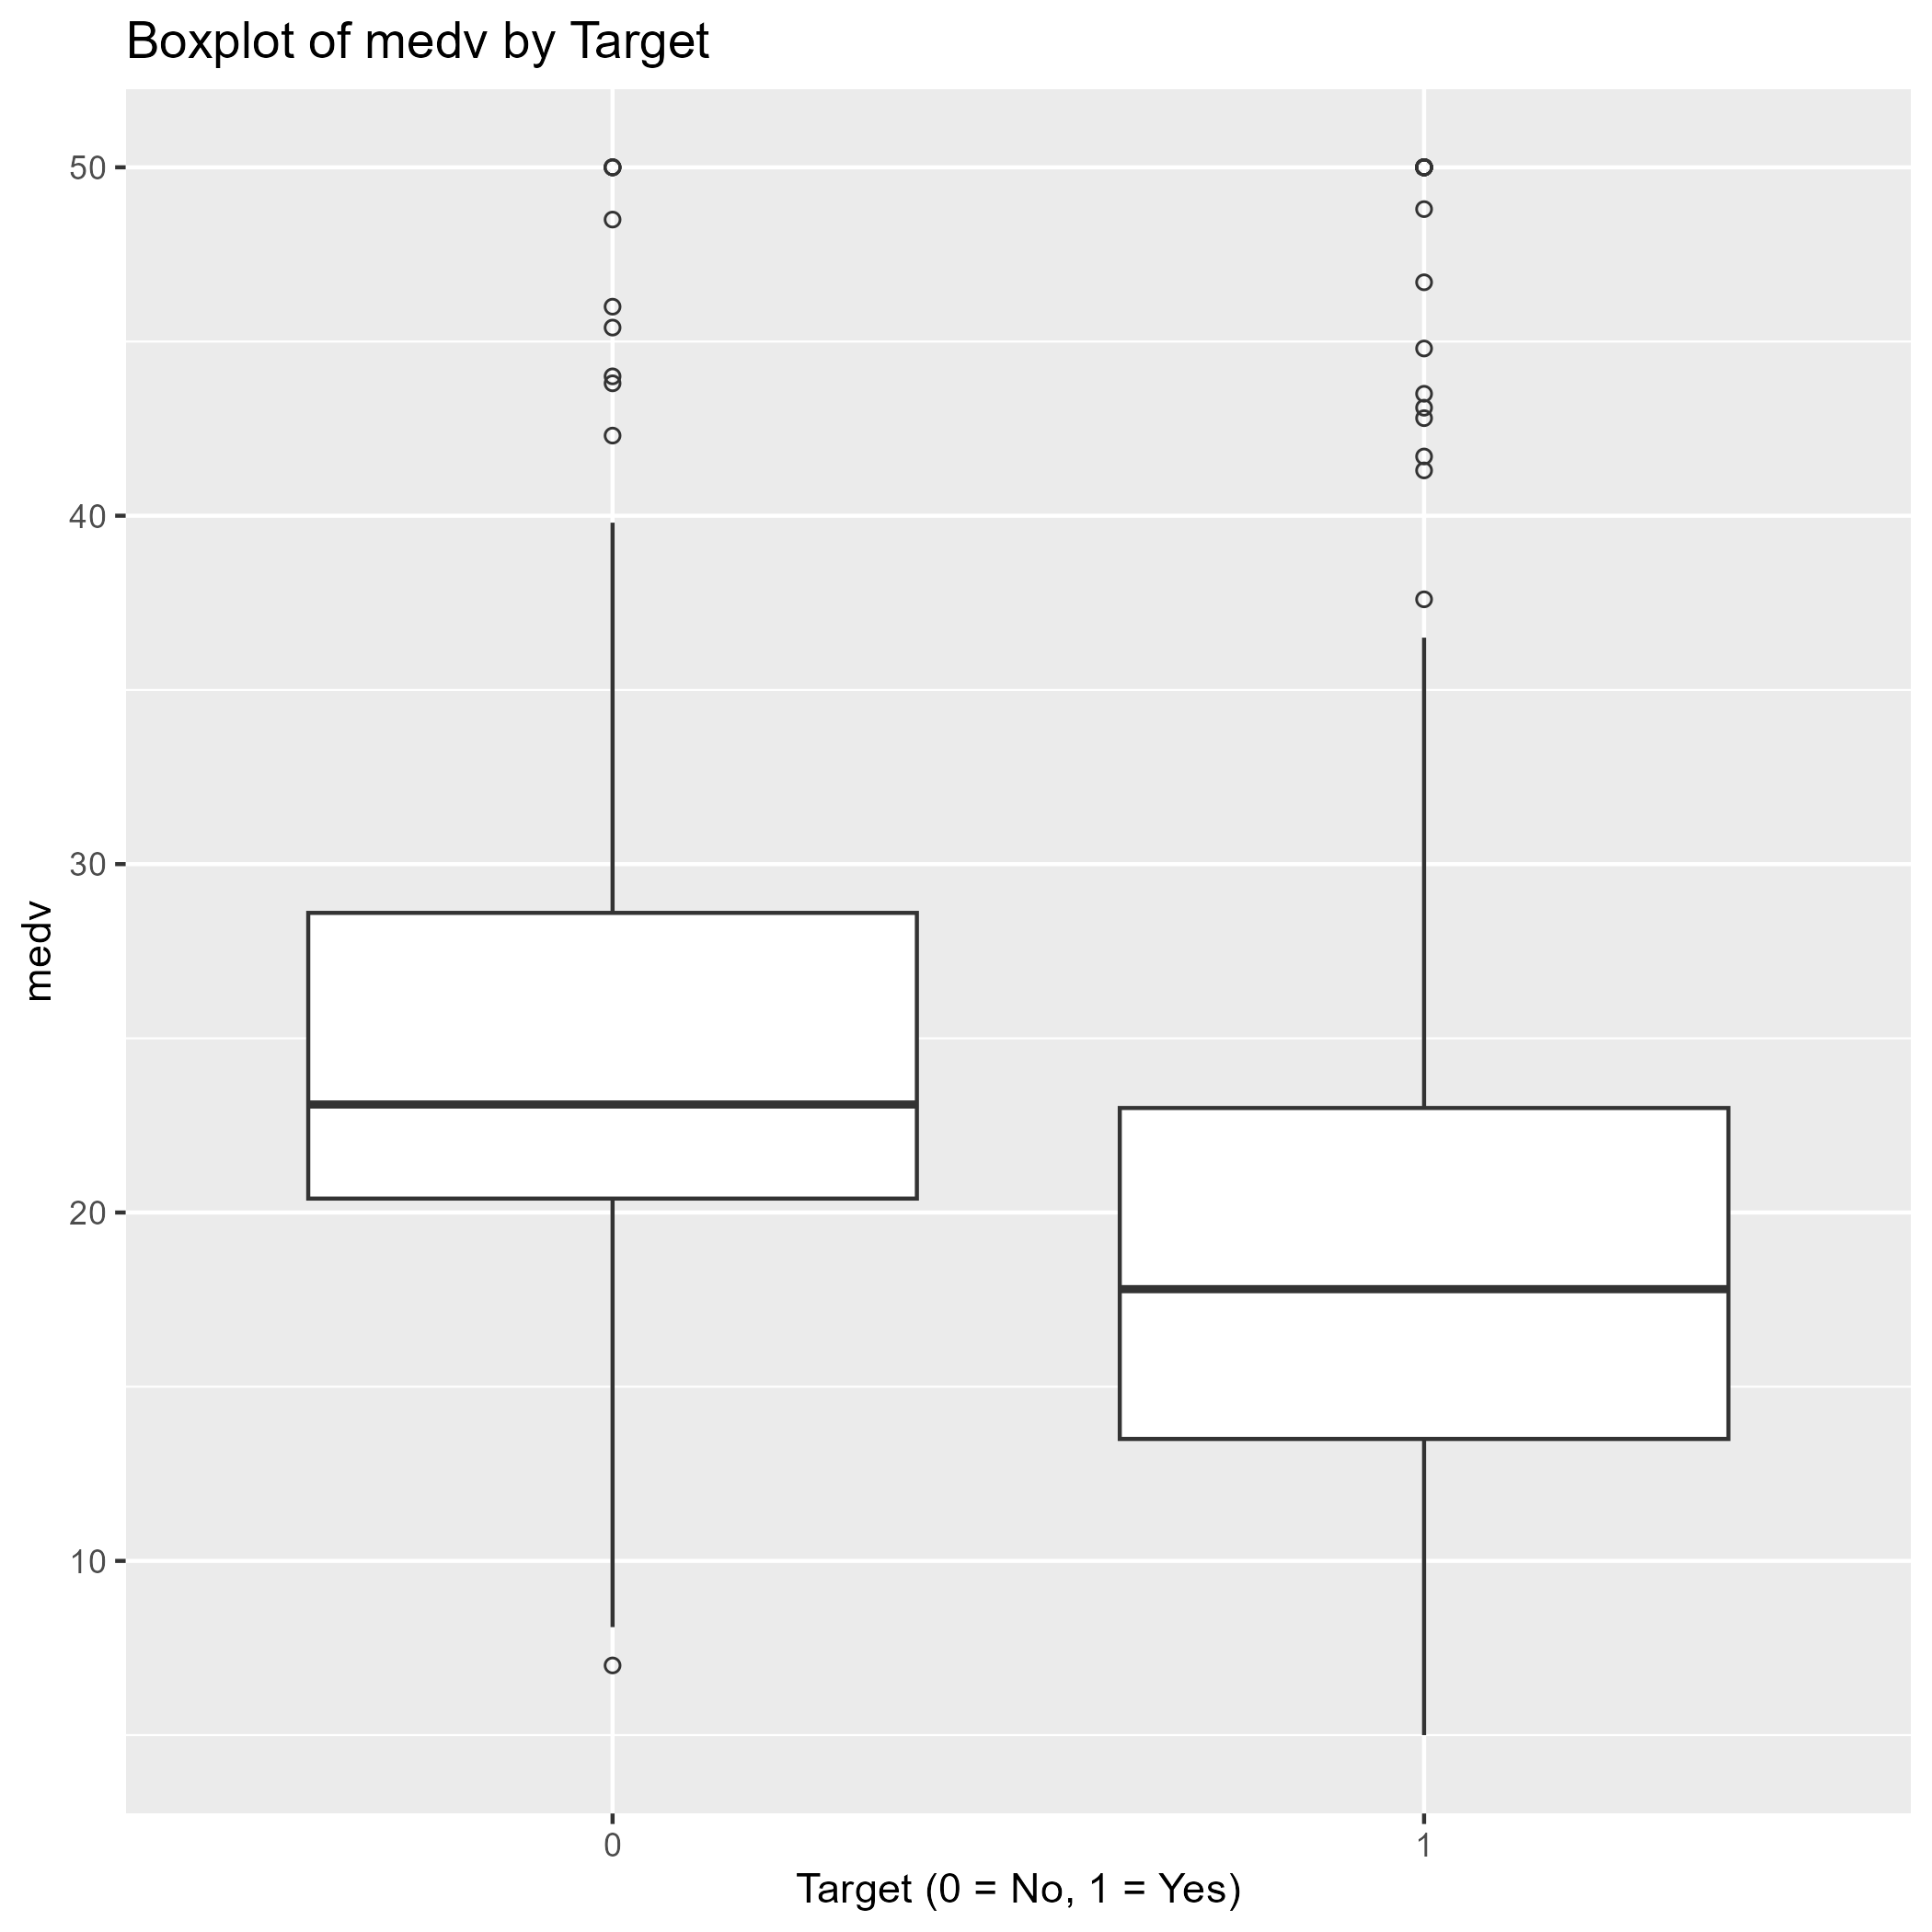
\includegraphics[keepaspectratio]{https://raw.githubusercontent.com/jhnboyy/CUNY_SPS_WORK/refs/heads/main/Spring2025/DATA621/DATA621_Homework3/images/Boxplotmedv_plot.png}}

In summation for data exploration, the target variable covering crime
rates seems to have meaningful relationships with several of the
predictors in the dataset. Additionally, non-target variables have
relationships with one another that should be considered for processing
and before modeling. The suggestions from this exploration hint that
zoning, environmental quality, infrastructure access, and socioeconomic
factors could all play a role in predicting crime levels.

\paragraph{Reading in Data}\label{reading-in-data}

\begin{Shaded}
\begin{Highlighting}[]
\DocumentationTok{\#\# Pushed the small amount of data to git, so reading in from there.}

\NormalTok{crime\_eval\_mod }\OtherTok{\textless{}{-}} \FunctionTok{read.csv}\NormalTok{(}\StringTok{"https://raw.githubusercontent.com/jhnboyy/CUNY\_SPS\_WORK/refs/heads/main/Spring2025/DATA621/DATA621\_Homework3/crime{-}evaluation{-}data\_modified.csv"}\NormalTok{)}

\NormalTok{crime\_train\_mod }\OtherTok{\textless{}{-}} \FunctionTok{read.csv}\NormalTok{(}\StringTok{"https://raw.githubusercontent.com/jhnboyy/CUNY\_SPS\_WORK/refs/heads/main/Spring2025/DATA621/DATA621\_Homework3/crime{-}training{-}data\_modified.csv"}\NormalTok{)}
\end{Highlighting}
\end{Shaded}

\subsubsection{Exploring the Training
Data}\label{exploring-the-training-data}

\begin{Shaded}
\begin{Highlighting}[]
\DocumentationTok{\#\# Summary of the Training Data}
\FunctionTok{print}\NormalTok{(}\FunctionTok{summary}\NormalTok{(crime\_train\_mod))}
\end{Highlighting}
\end{Shaded}

\begin{verbatim}
##        zn             indus             chas              nox        
##  Min.   :  0.00   Min.   : 0.460   Min.   :0.00000   Min.   :0.3890  
##  1st Qu.:  0.00   1st Qu.: 5.145   1st Qu.:0.00000   1st Qu.:0.4480  
##  Median :  0.00   Median : 9.690   Median :0.00000   Median :0.5380  
##  Mean   : 11.58   Mean   :11.105   Mean   :0.07082   Mean   :0.5543  
##  3rd Qu.: 16.25   3rd Qu.:18.100   3rd Qu.:0.00000   3rd Qu.:0.6240  
##  Max.   :100.00   Max.   :27.740   Max.   :1.00000   Max.   :0.8710  
##        rm             age              dis              rad       
##  Min.   :3.863   Min.   :  2.90   Min.   : 1.130   Min.   : 1.00  
##  1st Qu.:5.887   1st Qu.: 43.88   1st Qu.: 2.101   1st Qu.: 4.00  
##  Median :6.210   Median : 77.15   Median : 3.191   Median : 5.00  
##  Mean   :6.291   Mean   : 68.37   Mean   : 3.796   Mean   : 9.53  
##  3rd Qu.:6.630   3rd Qu.: 94.10   3rd Qu.: 5.215   3rd Qu.:24.00  
##  Max.   :8.780   Max.   :100.00   Max.   :12.127   Max.   :24.00  
##       tax           ptratio         lstat             medv      
##  Min.   :187.0   Min.   :12.6   Min.   : 1.730   Min.   : 5.00  
##  1st Qu.:281.0   1st Qu.:16.9   1st Qu.: 7.043   1st Qu.:17.02  
##  Median :334.5   Median :18.9   Median :11.350   Median :21.20  
##  Mean   :409.5   Mean   :18.4   Mean   :12.631   Mean   :22.59  
##  3rd Qu.:666.0   3rd Qu.:20.2   3rd Qu.:16.930   3rd Qu.:25.00  
##  Max.   :711.0   Max.   :22.0   Max.   :37.970   Max.   :50.00  
##      target      
##  Min.   :0.0000  
##  1st Qu.:0.0000  
##  Median :0.0000  
##  Mean   :0.4914  
##  3rd Qu.:1.0000  
##  Max.   :1.0000
\end{verbatim}

\begin{Shaded}
\begin{Highlighting}[]
\CommentTok{\# Double Checking for NA }
\FunctionTok{print}\NormalTok{(}\FunctionTok{colSums}\NormalTok{(}\FunctionTok{is.na}\NormalTok{(crime\_train\_mod))) }\CommentTok{\# No nulls to remove/ impute.}
\end{Highlighting}
\end{Shaded}

\begin{verbatim}
##      zn   indus    chas     nox      rm     age     dis     rad     tax ptratio 
##       0       0       0       0       0       0       0       0       0       0 
##   lstat    medv  target 
##       0       0       0
\end{verbatim}

\begin{Shaded}
\begin{Highlighting}[]
\FunctionTok{print}\NormalTok{(}\FunctionTok{nrow}\NormalTok{(crime\_train\_mod)) }\CommentTok{\#466 rows}
\end{Highlighting}
\end{Shaded}

\begin{verbatim}
## [1] 466
\end{verbatim}

\begin{Shaded}
\begin{Highlighting}[]
\DocumentationTok{\#\# Looping throuhg all of the continous columns, and plotting with target on the x axis. }
\ControlFlowTok{for}\NormalTok{ (col }\ControlFlowTok{in} \FunctionTok{c}\NormalTok{(}\FunctionTok{colnames}\NormalTok{(crime\_train\_mod }\SpecialCharTok{|\textgreater{}}\NormalTok{ dplyr}\SpecialCharTok{::}\FunctionTok{select}\NormalTok{(}\SpecialCharTok{{-}}\NormalTok{target,}\SpecialCharTok{{-}}\NormalTok{chas)))) \{}
  \CommentTok{\#print(col)}
\NormalTok{  box\_plot }\OtherTok{\textless{}{-}} \FunctionTok{ggplot}\NormalTok{(crime\_train\_mod, }\FunctionTok{aes}\NormalTok{(}\AttributeTok{x =} \FunctionTok{factor}\NormalTok{(target), }\AttributeTok{y =}\NormalTok{ .data[[col]])) }\SpecialCharTok{+}
    \FunctionTok{geom\_boxplot}\NormalTok{(}\AttributeTok{outlier.shape =} \DecValTok{1}\NormalTok{) }\SpecialCharTok{+}
    \FunctionTok{labs}\NormalTok{(}
      \AttributeTok{x =} \StringTok{"Target (0 = No, 1 = Yes)"}\NormalTok{,}
      \AttributeTok{y =}\NormalTok{ col,}
      \AttributeTok{title =} \FunctionTok{paste}\NormalTok{(}\StringTok{"Boxplot of"}\NormalTok{, col, }\StringTok{"by Target"}\NormalTok{)}
\NormalTok{    )}
  \CommentTok{\#print(box\_plot)}
  \CommentTok{\#ggsave(paste0("images/Boxplot",col,"\_plot.png"), plot = box\_plot, units = "in", dpi = 300)}

\NormalTok{\}}

\DocumentationTok{\#\# Based on these box plots, target\textquotesingle{}s relationship with other variables seems as follows: }
\CommentTok{\#{-} zn: Nearly all of the higher zoning values correlate with 0 values of target. Lower Crime, higher zoning value}
\CommentTok{\#{-} indus: the higher values for indus generally correlate with higher crime target values. Some exceptions.}
\CommentTok{\#{-} nox: higher nox values correlated with high crime target vals. }
\CommentTok{\#{-} rm: not much of an outlying pattern here.}
\CommentTok{\#{-} age: slight trend of higher age of area, higher crime target values.}
\CommentTok{\#{-} dis: higher values seem to be lower crime, some exceptions.}
\CommentTok{\#{-} rad: higher values associated with higher crime.}
\CommentTok{\#{-} tax: higher values associated with higher crime, some exceptions.}
\CommentTok{\#{-} ptratio: very slight correlation, not too definitive. Higher ptratio, maybe higher crime.}
\CommentTok{\#{-} lstat: slight correlation, high crime with higher lstat values}
\CommentTok{\#{-} medv: weak correlation lower crime, hiwher medv number. }
\end{Highlighting}
\end{Shaded}

\paragraph{GGPairs Visual for Training
Data}\label{ggpairs-visual-for-training-data}

\begin{Shaded}
\begin{Highlighting}[]
\DocumentationTok{\#\# Taking a look at how the variables relate to one another via ggpairs.}

\CommentTok{\#p \textless{}{-} }
  \FunctionTok{ggpairs}\NormalTok{(crime\_train\_mod,}\AttributeTok{progress =} \ConstantTok{FALSE}\NormalTok{) }\SpecialCharTok{+}\FunctionTok{theme\_minimal}\NormalTok{(}\AttributeTok{base\_size=}\DecValTok{9}\NormalTok{) }\SpecialCharTok{+}
  \FunctionTok{theme}\NormalTok{(}\AttributeTok{axis.text.x =} \FunctionTok{element\_text}\NormalTok{(}\AttributeTok{angle =} \DecValTok{45}\NormalTok{, }\AttributeTok{hjust =} \DecValTok{1}\NormalTok{),}
                                      \AttributeTok{strip.text.x =} \FunctionTok{element\_text}\NormalTok{(}\AttributeTok{angle =} \DecValTok{90}\NormalTok{, }\AttributeTok{hjust =} \DecValTok{1}\NormalTok{),}
                                     \AttributeTok{strip.text.y =} \FunctionTok{element\_text}\NormalTok{(}\AttributeTok{angle =} \DecValTok{0}\NormalTok{, }\AttributeTok{hjust =} \DecValTok{1}\NormalTok{))}
\end{Highlighting}
\end{Shaded}

\pandocbounded{\includegraphics[keepaspectratio]{DATA621_Homework3_Group2_Final_files/figure-latex/ggpairs-1.pdf}}

\begin{Shaded}
\begin{Highlighting}[]
\DocumentationTok{\#\# Saving Image for reference in PDF \#}
\CommentTok{\#ggsave("images/ggpairs\_plot.png", plot = p, width = 15, height = 20, units = "in", dpi = 300)}

\DocumentationTok{\#\# The takeaways that i see for the GGpairs chart for iteration / relationships between variables:}
\DocumentationTok{\#\#  {-} There is a negative relationship between zn(Large residential Lot Zoned Land) and indus (proportion of non retail businesses). Makes sense as the larger the residential land}
\DocumentationTok{\#\#    zoning is, the less likely there will be non retail / industrial type businesses also prominent in the area. }
\DocumentationTok{\#\#  {-} Similar negative relationship for NOX and ZN, which makes sense because there is also a direct relationship with indus and nox. Im assuming NOX is an industrial emission.}
\DocumentationTok{\#\#  {-} Negative relationship btwn zn and age, which would imply that larger residential type living zone is a newer development. Where older development buildings are zoned smaller}
\DocumentationTok{\#\#  {-} Direct relationship with age and nox as well as indus, which i would guess is that neighborhoods with older building areas, have more industrial development and nox emission}
\DocumentationTok{\#\#  {-} Steep neg. relationship with age and rm. Older buildings smaller so older buildings, have less rooms.}
\DocumentationTok{\#\#  {-} Age has negative relationship with zn, and positive one with indus}
\DocumentationTok{\#\#  {-} dis column, the weighted dist. to employment centers, has a negative relationship with: nox, age, indus. While dis has a positive relationship with zn.}
\DocumentationTok{\#\#  {-} lstat, lower status population, has neg. relationship with zn, rm and dis. While lstat has pos. relationship with: age, indus, nox, and a slight one with ptratio}
\DocumentationTok{\#\#  {-} medv, med. value of owner{-}occupied home, has a neg. relationship with: indus, nox, lstat, and slight neg. with age. medv has positive rel. with: dis, rm, zn.}
\end{Highlighting}
\end{Shaded}

\paragraph{Correlation Matrix Check}\label{correlation-matrix-check}

\begin{Shaded}
\begin{Highlighting}[]
\CommentTok{\# Cor Matrics with no dummy var chas or binary target }
\NormalTok{cor\_matrix }\OtherTok{\textless{}{-}} \FunctionTok{cor}\NormalTok{(crime\_train\_mod }\SpecialCharTok{|\textgreater{}}\NormalTok{ dplyr}\SpecialCharTok{::}\FunctionTok{select}\NormalTok{(}\SpecialCharTok{{-}}\NormalTok{target,}\SpecialCharTok{{-}}\NormalTok{chas), }\AttributeTok{use =} \StringTok{"complete.obs"}\NormalTok{)}
\FunctionTok{print}\NormalTok{(cor\_matrix)}
\end{Highlighting}
\end{Shaded}

\begin{verbatim}
##                 zn      indus        nox         rm        age        dis
## zn       1.0000000 -0.5382664 -0.5170452  0.3198141 -0.5725805  0.6601243
## indus   -0.5382664  1.0000000  0.7596301 -0.3927118  0.6395818 -0.7036189
## nox     -0.5170452  0.7596301  1.0000000 -0.2954897  0.7351278 -0.7688840
## rm       0.3198141 -0.3927118 -0.2954897  1.0000000 -0.2328125  0.1990158
## age     -0.5725805  0.6395818  0.7351278 -0.2328125  1.0000000 -0.7508976
## dis      0.6601243 -0.7036189 -0.7688840  0.1990158 -0.7508976  1.0000000
## rad     -0.3154812  0.6006284  0.5958298 -0.2084457  0.4603143 -0.4949919
## tax     -0.3192841  0.7322292  0.6538780 -0.2969343  0.5121245 -0.5342546
## ptratio -0.3910357  0.3946898  0.1762687 -0.3603471  0.2554479 -0.2333394
## lstat   -0.4329925  0.6071102  0.5962426 -0.6320245  0.6056200 -0.5075280
## medv     0.3767171 -0.4961743 -0.4301227  0.7053368 -0.3781560  0.2566948
##                rad        tax    ptratio      lstat       medv
## zn      -0.3154812 -0.3192841 -0.3910357 -0.4329925  0.3767171
## indus    0.6006284  0.7322292  0.3946898  0.6071102 -0.4961743
## nox      0.5958298  0.6538780  0.1762687  0.5962426 -0.4301227
## rm      -0.2084457 -0.2969343 -0.3603471 -0.6320245  0.7053368
## age      0.4603143  0.5121245  0.2554479  0.6056200 -0.3781560
## dis     -0.4949919 -0.5342546 -0.2333394 -0.5075280  0.2566948
## rad      1.0000000  0.9064632  0.4714516  0.5031013 -0.3976683
## tax      0.9064632  1.0000000  0.4744223  0.5641886 -0.4900329
## ptratio  0.4714516  0.4744223  1.0000000  0.3773560 -0.5159153
## lstat    0.5031013  0.5641886  0.3773560  1.0000000 -0.7358008
## medv    -0.3976683 -0.4900329 -0.5159153 -0.7358008  1.0000000
\end{verbatim}

\begin{Shaded}
\begin{Highlighting}[]
\CommentTok{\# This tracks with what i outlined in my notes on the ggpairs plot.}

\DocumentationTok{\#\# Looking here in order to find potential agg index variables to make. }
\DocumentationTok{\#\# Potential colinear type relationships here: }
\CommentTok{\# indus {-}\textgreater{} nox, {-} dis}
\CommentTok{\# nox {-}\textgreater{} {-}dis, age (age gives diff info though)}
\CommentTok{\# age {-}\textgreater{} dis}
\CommentTok{\# rad {-}\textgreater{} tax (super high correlation)}
\CommentTok{\# lstat {-}\textgreater{} {-} medv}
\end{Highlighting}
\end{Shaded}

\subsubsection{2. DATA PREPARATION (25
Points)}\label{data-preparation-25-points}

Describe how you have transformed the data by changing the original
variables or creating new variables. If you did transform the data or
create new variables, discuss why you did this. Here are some possible
transformations. a. Fix missing values (maybe with a Mean or Median
value) b. Create flags to suggest if a variable was missing c.~Transform
data by putting it into buckets d.~Mathematical transforms such as log
or square root (or, use Box-Cox) e. Combine variables (such as ratios or
adding or multiplying) to create new variables

\paragraph{Check For Missing Values}\label{check-for-missing-values}

We check for missing values in both training and evaluation crime
datasets by inspecting the extent of missing data in each by computing
and plotting the number of missing values per variable. There are
\textbf{no missing values} in our training and evaluation datasets and
no further treatment is needed.

Logistic regression assumes that the input data is complete and does not
handle missing values natively. If missing values are not addressed,
this can lead to biased parameter estimates, reduced model accuracy, and
invalid inference. Ignoring missing values might exclude important
observations, potentially distorting the relationship between predictors
and the binary outcomes. Also pattern of missingness may contain
important information about the underlying data-generating process that
could be relevant to the crime prediction logistic regression model. We
can use imputation, deletion, or others methods to model coefficients
accurately,

\begin{Shaded}
\begin{Highlighting}[]
\FunctionTok{library}\NormalTok{(ggplot2)}
\FunctionTok{library}\NormalTok{(gridExtra)}

\CommentTok{\# Load datasets}
\NormalTok{crime\_eval\_mod }\OtherTok{\textless{}{-}} \FunctionTok{read.csv}\NormalTok{(}\StringTok{"https://raw.githubusercontent.com/jhnboyy/CUNY\_SPS\_WORK/refs/heads/main/Spring2025/DATA621/DATA621\_Homework3/crime{-}evaluation{-}data\_modified.csv"}\NormalTok{)}
\NormalTok{crime\_train\_mod }\OtherTok{\textless{}{-}} \FunctionTok{read.csv}\NormalTok{(}\StringTok{"https://raw.githubusercontent.com/jhnboyy/CUNY\_SPS\_WORK/refs/heads/main/Spring2025/DATA621/DATA621\_Homework3/crime{-}training{-}data\_modified.csv"}\NormalTok{)}

\CommentTok{\# Compute missing value counts for training data}
\NormalTok{missing\_train }\OtherTok{\textless{}{-}} \FunctionTok{sapply}\NormalTok{(crime\_train\_mod, }\ControlFlowTok{function}\NormalTok{(x) }\FunctionTok{sum}\NormalTok{(}\FunctionTok{is.na}\NormalTok{(x)))}
\NormalTok{missing\_train\_df }\OtherTok{\textless{}{-}} \FunctionTok{data.frame}\NormalTok{(}\AttributeTok{Variable =} \FunctionTok{names}\NormalTok{(missing\_train), }\AttributeTok{MissingCount =}\NormalTok{ missing\_train)}

\CommentTok{\# Compute missing value counts for evaluation data}
\NormalTok{missing\_eval }\OtherTok{\textless{}{-}} \FunctionTok{sapply}\NormalTok{(crime\_eval\_mod, }\ControlFlowTok{function}\NormalTok{(x) }\FunctionTok{sum}\NormalTok{(}\FunctionTok{is.na}\NormalTok{(x)))}
\NormalTok{missing\_eval\_df }\OtherTok{\textless{}{-}} \FunctionTok{data.frame}\NormalTok{(}\AttributeTok{Variable =} \FunctionTok{names}\NormalTok{(missing\_eval), }\AttributeTok{MissingCount =}\NormalTok{ missing\_eval)}

\CommentTok{\# Create plots}
\NormalTok{plot\_train }\OtherTok{\textless{}{-}} \FunctionTok{ggplot}\NormalTok{(missing\_train\_df, }\FunctionTok{aes}\NormalTok{(}\AttributeTok{x =} \FunctionTok{reorder}\NormalTok{(Variable, MissingCount), }\AttributeTok{y =}\NormalTok{ MissingCount)) }\SpecialCharTok{+}
  \FunctionTok{geom\_bar}\NormalTok{(}\AttributeTok{stat =} \StringTok{"identity"}\NormalTok{, }\AttributeTok{fill =} \StringTok{"red"}\NormalTok{) }\SpecialCharTok{+}
  \FunctionTok{labs}\NormalTok{(}\AttributeTok{title =} \StringTok{"Missing Values: Training Data"}\NormalTok{, }\AttributeTok{x =} \StringTok{"Variable"}\NormalTok{, }\AttributeTok{y =} \StringTok{"Count"}\NormalTok{) }\SpecialCharTok{+}
  \FunctionTok{coord\_flip}\NormalTok{() }\SpecialCharTok{+}
  \FunctionTok{theme\_minimal}\NormalTok{()}

\NormalTok{plot\_eval }\OtherTok{\textless{}{-}} \FunctionTok{ggplot}\NormalTok{(missing\_eval\_df, }\FunctionTok{aes}\NormalTok{(}\AttributeTok{x =} \FunctionTok{reorder}\NormalTok{(Variable, MissingCount), }\AttributeTok{y =}\NormalTok{ MissingCount)) }\SpecialCharTok{+}
  \FunctionTok{geom\_bar}\NormalTok{(}\AttributeTok{stat =} \StringTok{"identity"}\NormalTok{, }\AttributeTok{fill =} \StringTok{"red"}\NormalTok{) }\SpecialCharTok{+}
  \FunctionTok{labs}\NormalTok{(}\AttributeTok{title =} \StringTok{"Missing Values: Evaluation Data"}\NormalTok{, }\AttributeTok{x =} \StringTok{"Variable"}\NormalTok{, }\AttributeTok{y =} \StringTok{"Count"}\NormalTok{) }\SpecialCharTok{+}
  \FunctionTok{coord\_flip}\NormalTok{() }\SpecialCharTok{+}
  \FunctionTok{theme\_minimal}\NormalTok{()}

\FunctionTok{grid.arrange}\NormalTok{(plot\_train, plot\_eval, }\AttributeTok{ncol =} \DecValTok{2}\NormalTok{)}
\end{Highlighting}
\end{Shaded}

\pandocbounded{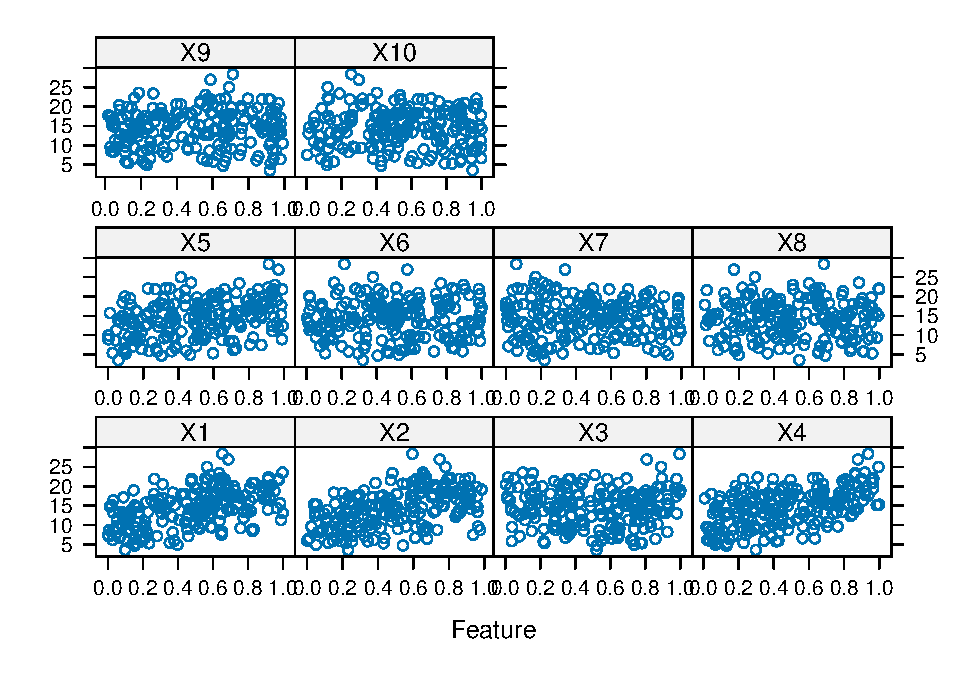
\includegraphics[keepaspectratio]{DATA621_Homework3_Group2_Final_files/figure-latex/unnamed-chunk-1-1.pdf}}

\paragraph{Address Skewness}\label{address-skewness}

We addresses skewness in a set of variables by applying a Box‑Cox
transformation. For each skewed variable =, \textbf{``zn'', ``dis'',
``lstat'', ``medv''}, we adjust the data to ensure all values are
positive by adding an offset if necessary and compute the optimal lambda
parameter using the Box‑Cox method. The computed lambda is used to
transform the variable in both the training and evaluation datasets.

Our transformation result in ``medv'' (median home value) and ``lstat''
(\% lower status population) are positively skewed but become more
symmetric with λ=0.2; ``dis'' (distance to employment centers) is also
right-skewed but transforms well with λ=-0.1; and ``zn'' (residential
land zoning) has an extreme positive skew that becomes more balanced
with λ=-0.9.

Transforming skewed variables is important in logistic regression
because the models perform better when the predictors are symmetrically
distributed. Skewness can lead to unstable coefficient estimates, affect
the interpretability of model parameters, and ultimately reduce
predictive performance. The Box‑Cox transformation helps to stabilize
variance and reduce the influence of outliers.

\begin{Shaded}
\begin{Highlighting}[]
\FunctionTok{library}\NormalTok{(MASS)}
\FunctionTok{library}\NormalTok{(gridExtra)}
\FunctionTok{library}\NormalTok{(ggplot2)}

\CommentTok{\# Identify skewed variables}
\NormalTok{skewed\_vars }\OtherTok{\textless{}{-}} \FunctionTok{c}\NormalTok{(}\StringTok{"zn"}\NormalTok{, }\StringTok{"dis"}\NormalTok{, }\StringTok{"lstat"}\NormalTok{, }\StringTok{"medv"}\NormalTok{)}

\CommentTok{\# Prepare list for plots}
\NormalTok{transformation\_plots }\OtherTok{\textless{}{-}} \FunctionTok{list}\NormalTok{()}

\CommentTok{\# Loop through each skewed variable}
\ControlFlowTok{for}\NormalTok{ (var }\ControlFlowTok{in}\NormalTok{ skewed\_vars) \{}
  \CommentTok{\# Adjust training data so all values are positive}
\NormalTok{  x }\OtherTok{\textless{}{-}}\NormalTok{ crime\_train\_mod[[var]]}
\NormalTok{  offset }\OtherTok{\textless{}{-}} \FunctionTok{pmax}\NormalTok{(}\DecValTok{1} \SpecialCharTok{{-}} \FunctionTok{min}\NormalTok{(x, }\AttributeTok{na.rm =} \ConstantTok{TRUE}\NormalTok{), }\DecValTok{0}\NormalTok{)}
\NormalTok{  x\_adj }\OtherTok{\textless{}{-}}\NormalTok{ x }\SpecialCharTok{+}\NormalTok{ offset}
  
  \CommentTok{\# Compute Box{-}Cox lambda}
\NormalTok{  bc }\OtherTok{\textless{}{-}} \FunctionTok{boxcox}\NormalTok{(x\_adj }\SpecialCharTok{\textasciitilde{}} \DecValTok{1}\NormalTok{, }\AttributeTok{lambda =} \FunctionTok{seq}\NormalTok{(}\SpecialCharTok{{-}}\DecValTok{2}\NormalTok{, }\DecValTok{2}\NormalTok{, }\AttributeTok{by =} \FloatTok{0.1}\NormalTok{), }\AttributeTok{plotit =} \ConstantTok{FALSE}\NormalTok{)}
\NormalTok{  lambda }\OtherTok{\textless{}{-}}\NormalTok{ bc}\SpecialCharTok{$}\NormalTok{x[}\FunctionTok{which.max}\NormalTok{(bc}\SpecialCharTok{$}\NormalTok{y)]}
  
  \CommentTok{\# Apply Box{-}Cox transformation to the training data}
\NormalTok{  train\_trans }\OtherTok{\textless{}{-}}\NormalTok{ (x\_adj}\SpecialCharTok{\^{}}\NormalTok{lambda }\SpecialCharTok{{-}} \DecValTok{1}\NormalTok{) }\SpecialCharTok{/}\NormalTok{ lambda}
  
  \CommentTok{\# Adjust and transform evaluation data}
\NormalTok{  x\_eval }\OtherTok{\textless{}{-}}\NormalTok{ crime\_eval\_mod[[var]]}
\NormalTok{  offset\_eval }\OtherTok{\textless{}{-}} \FunctionTok{pmax}\NormalTok{(}\DecValTok{1} \SpecialCharTok{{-}} \FunctionTok{min}\NormalTok{(x\_eval, }\AttributeTok{na.rm =} \ConstantTok{TRUE}\NormalTok{), }\DecValTok{0}\NormalTok{)}
\NormalTok{  x\_eval\_adj }\OtherTok{\textless{}{-}}\NormalTok{ x\_eval }\SpecialCharTok{+}\NormalTok{ offset\_eval}
\NormalTok{  eval\_trans }\OtherTok{\textless{}{-}}\NormalTok{ (x\_eval\_adj}\SpecialCharTok{\^{}}\NormalTok{lambda }\SpecialCharTok{{-}} \DecValTok{1}\NormalTok{) }\SpecialCharTok{/}\NormalTok{ lambda}
  
  \CommentTok{\# Save transformed variables}
\NormalTok{  crime\_train\_prep }\OtherTok{\textless{}{-}}\NormalTok{ crime\_train\_mod}
\NormalTok{  crime\_train\_prep[[}\FunctionTok{paste0}\NormalTok{(var, }\StringTok{"\_trans"}\NormalTok{)]] }\OtherTok{\textless{}{-}}\NormalTok{ train\_trans}
\NormalTok{  crime\_eval\_prep }\OtherTok{\textless{}{-}}\NormalTok{ crime\_eval\_mod}
\NormalTok{  crime\_eval\_prep[[}\FunctionTok{paste0}\NormalTok{(var, }\StringTok{"\_trans"}\NormalTok{)]] }\OtherTok{\textless{}{-}}\NormalTok{ eval\_trans}
  
  \CommentTok{\# Create the "before" density plot}
\NormalTok{  before\_plot }\OtherTok{\textless{}{-}} \FunctionTok{ggplot}\NormalTok{(crime\_train\_mod, }\FunctionTok{aes}\NormalTok{(}\AttributeTok{x =}\NormalTok{ .data[[var]])) }\SpecialCharTok{+}
    \FunctionTok{geom\_density}\NormalTok{(}\AttributeTok{fill =} \StringTok{"steelblue"}\NormalTok{, }\AttributeTok{alpha =} \FloatTok{0.7}\NormalTok{) }\SpecialCharTok{+}
    \FunctionTok{labs}\NormalTok{(}\AttributeTok{title =} \FunctionTok{paste}\NormalTok{(}\StringTok{"Before:"}\NormalTok{, var),}
         \AttributeTok{x =}\NormalTok{ var, }\AttributeTok{y =} \StringTok{"Density"}\NormalTok{) }\SpecialCharTok{+}
    \FunctionTok{theme\_minimal}\NormalTok{(}\AttributeTok{base\_size =} \DecValTok{9}\NormalTok{)}
  
  \CommentTok{\# Create the "after" density plot}
\NormalTok{  after\_plot }\OtherTok{\textless{}{-}} \FunctionTok{ggplot}\NormalTok{(crime\_train\_prep, }\FunctionTok{aes}\NormalTok{(}\AttributeTok{x =}\NormalTok{ .data[[}\FunctionTok{paste0}\NormalTok{(var, }\StringTok{"\_trans"}\NormalTok{)]])) }\SpecialCharTok{+}
    \FunctionTok{geom\_density}\NormalTok{(}\AttributeTok{fill =} \StringTok{"gray"}\NormalTok{, }\AttributeTok{alpha =} \FloatTok{0.7}\NormalTok{) }\SpecialCharTok{+}
    \FunctionTok{labs}\NormalTok{(}\AttributeTok{title =} \FunctionTok{paste}\NormalTok{(}\StringTok{"After: Box{-}Cox (λ ="}\NormalTok{, }\FunctionTok{round}\NormalTok{(lambda, }\DecValTok{2}\NormalTok{), }\StringTok{") Transform"}\NormalTok{),}
         \AttributeTok{x =} \FunctionTok{paste0}\NormalTok{(var, }\StringTok{"\_trans"}\NormalTok{), }\AttributeTok{y =} \StringTok{"Density"}\NormalTok{) }\SpecialCharTok{+}
    \FunctionTok{theme\_minimal}\NormalTok{(}\AttributeTok{base\_size =} \DecValTok{9}\NormalTok{)}
  
  \CommentTok{\# Arrange the before and after plots side by side and store in the list}
\NormalTok{  transformation\_plots[[var]] }\OtherTok{\textless{}{-}} \FunctionTok{grid.arrange}\NormalTok{(before\_plot, after\_plot, }\AttributeTok{ncol =} \DecValTok{2}\NormalTok{)}
\NormalTok{\}}
\end{Highlighting}
\end{Shaded}

\pandocbounded{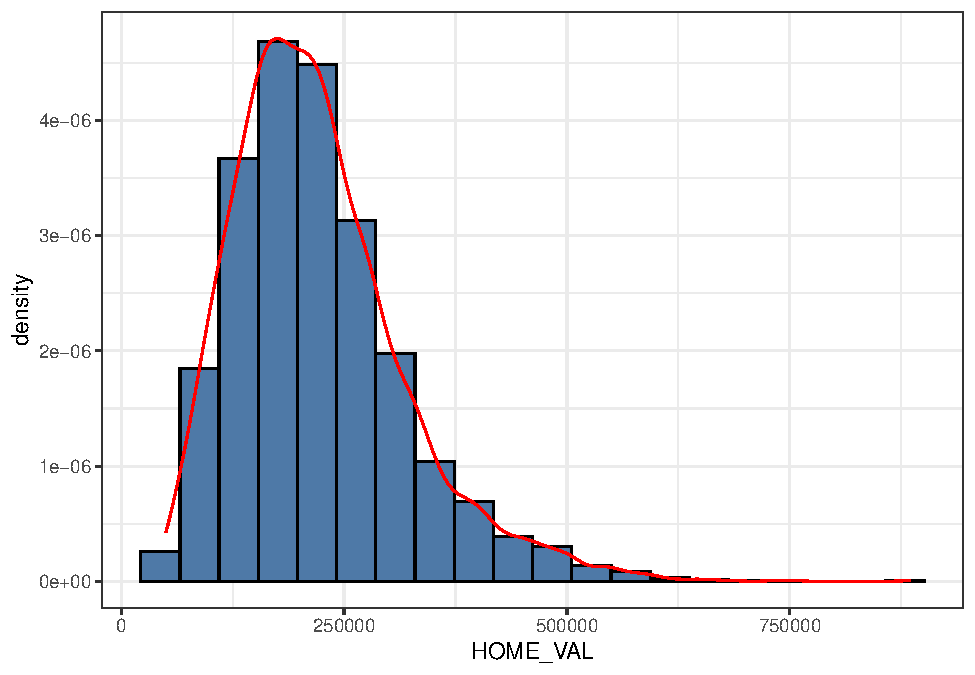
\includegraphics[keepaspectratio]{DATA621_Homework3_Group2_Final_files/figure-latex/unnamed-chunk-2-1.pdf}}
\pandocbounded{\includegraphics[keepaspectratio]{DATA621_Homework3_Group2_Final_files/figure-latex/unnamed-chunk-2-2.pdf}}
\pandocbounded{\includegraphics[keepaspectratio]{DATA621_Homework3_Group2_Final_files/figure-latex/unnamed-chunk-2-3.pdf}}
\pandocbounded{\includegraphics[keepaspectratio]{DATA621_Homework3_Group2_Final_files/figure-latex/unnamed-chunk-2-4.pdf}}

\paragraph{Check for
Multicollinearity}\label{check-for-multicollinearity}

We evaluate multicollinearity among predictor variables using the
Variance Inflation Factor (VIF). After fitting a logistic regression
model with all available predictors, we compute the VIF for each
variable to assess how much the variance of each estimated coefficient
is inflated due to linear relationships with other predictors. A VIF
value greater than 5 indicates high (and potentially problematic)
multicollinearity.

Multicollinearity can impact the stability and interpretability of
logistic regression models. When predictors are highly
correlated,estimating their individual contributions to the outcome
variable is difficult because their effects may be confounded. This can
lead to inflated standard errors, unreliable coefficient estimates, and
misleading inference, In our training date, \textbf{rm (average number
of rooms)} and \textbf{medv (median home value)} have VIF values of 5.81
and 8.12, respectively; these variables may be collinear with others in
the model. To address collinearity, we may need to drop or combine
variables to create an interpretable logistic regression model.

\begin{Shaded}
\begin{Highlighting}[]
\FunctionTok{library}\NormalTok{(car)}

\CommentTok{\# Check for multicollinearity with Variance Inflation Factor}
\NormalTok{initial\_model }\OtherTok{\textless{}{-}} \FunctionTok{glm}\NormalTok{(target }\SpecialCharTok{\textasciitilde{}}\NormalTok{ . , }\AttributeTok{data=}\NormalTok{crime\_train\_mod, }\AttributeTok{family=}\NormalTok{binomial)}
\NormalTok{vif\_results }\OtherTok{\textless{}{-}} \FunctionTok{vif}\NormalTok{(initial\_model)}
\FunctionTok{print}\NormalTok{(}\StringTok{"Variance Inflation Factors:"}\NormalTok{)}
\end{Highlighting}
\end{Shaded}

\begin{verbatim}
## [1] "Variance Inflation Factors:"
\end{verbatim}

\begin{Shaded}
\begin{Highlighting}[]
\FunctionTok{print}\NormalTok{(vif\_results)}
\end{Highlighting}
\end{Shaded}

\begin{verbatim}
##       zn    indus     chas      nox       rm      age      dis      rad 
## 1.823146 2.682271 1.241479 4.160497 5.813851 2.569961 3.887981 1.942967 
##      tax  ptratio    lstat     medv 
## 2.144040 2.275557 2.642656 8.122037
\end{verbatim}

\begin{Shaded}
\begin{Highlighting}[]
\CommentTok{\# Display variables with high VIF (\textgreater{}5 has high multicollinearity)}
\NormalTok{high\_vif }\OtherTok{\textless{}{-}}\NormalTok{ vif\_results[vif\_results }\SpecialCharTok{\textgreater{}} \DecValTok{5}\NormalTok{]}

\FunctionTok{print}\NormalTok{(}\StringTok{"Variables with high multicollinearity:"}\NormalTok{)}
\end{Highlighting}
\end{Shaded}

\begin{verbatim}
## [1] "Variables with high multicollinearity:"
\end{verbatim}

\begin{Shaded}
\begin{Highlighting}[]
\FunctionTok{print}\NormalTok{(high\_vif)}
\end{Highlighting}
\end{Shaded}

\begin{verbatim}
##       rm     medv 
## 5.813851 8.122037
\end{verbatim}

\begin{Shaded}
\begin{Highlighting}[]
\CommentTok{\# Visualize the VIF results}
\NormalTok{vif\_df }\OtherTok{\textless{}{-}} \FunctionTok{data.frame}\NormalTok{(}
  \AttributeTok{Variable =} \FunctionTok{names}\NormalTok{(vif\_results),}
  \AttributeTok{VIF =} \FunctionTok{as.numeric}\NormalTok{(vif\_results))}
\NormalTok{vif\_df }\OtherTok{\textless{}{-}}\NormalTok{ vif\_df[}\FunctionTok{order}\NormalTok{(}\SpecialCharTok{{-}}\NormalTok{vif\_df}\SpecialCharTok{$}\NormalTok{VIF),]}

\FunctionTok{ggplot}\NormalTok{(vif\_df, }\FunctionTok{aes}\NormalTok{(}\AttributeTok{x =} \FunctionTok{reorder}\NormalTok{(Variable, VIF), }\AttributeTok{y =}\NormalTok{ VIF)) }\SpecialCharTok{+}
  \FunctionTok{geom\_bar}\NormalTok{(}\AttributeTok{stat =} \StringTok{"identity"}\NormalTok{, }\AttributeTok{fill =} \StringTok{"steelblue"}\NormalTok{) }\SpecialCharTok{+}
  \FunctionTok{geom\_hline}\NormalTok{(}\AttributeTok{yintercept =} \DecValTok{5}\NormalTok{, }\AttributeTok{linetype =} \StringTok{"dashed"}\NormalTok{, }\AttributeTok{color =} \StringTok{"orange"}\NormalTok{) }\SpecialCharTok{+}
  \FunctionTok{labs}\NormalTok{(}\AttributeTok{title =} \StringTok{"Variance Inflation Factors (VIF) for Predictor Variables"}\NormalTok{,}
       \AttributeTok{subtitle =} \StringTok{"VIF \textgreater{} 5 (High Multicollinearity)"}\NormalTok{,}
       \AttributeTok{x =} \StringTok{"Variables"}\NormalTok{, }\AttributeTok{y =} \StringTok{"VIF"}\NormalTok{) }\SpecialCharTok{+}
  \FunctionTok{coord\_flip}\NormalTok{() }\SpecialCharTok{+}
  \FunctionTok{theme\_minimal}\NormalTok{()}
\end{Highlighting}
\end{Shaded}

\pandocbounded{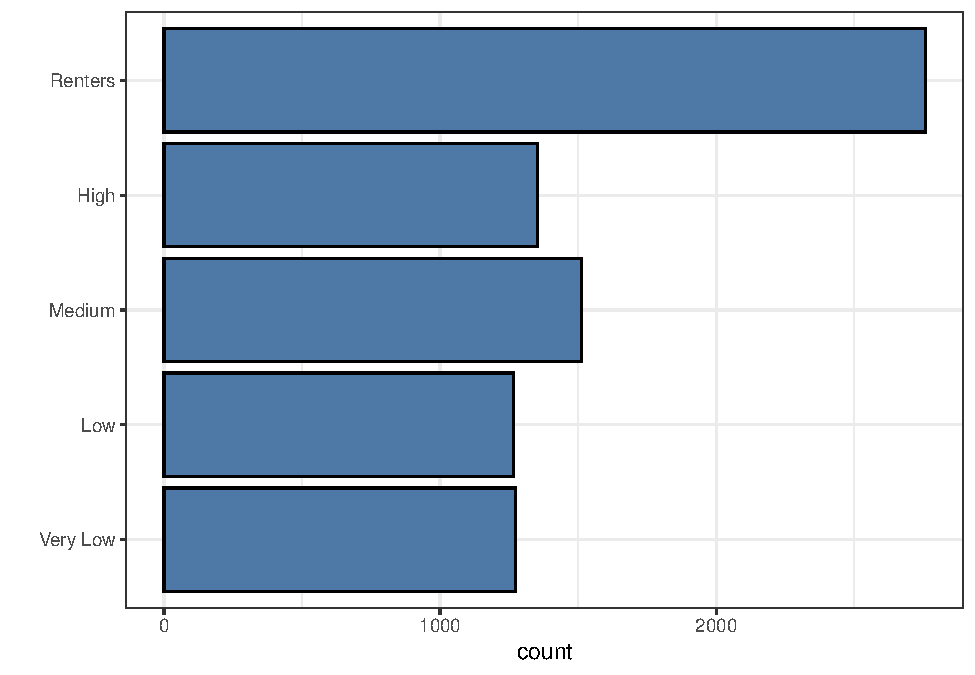
\includegraphics[keepaspectratio]{DATA621_Homework3_Group2_Final_files/figure-latex/unnamed-chunk-3-1.pdf}}

\paragraph{Create Composite
Predictors}\label{create-composite-predictors}

Here we construct and visualize four composite combined indices,
\textbf{env\_index, ses\_index, urban\_index, and infra\_index} that
aggregate predictors into interpretable combinations related to
environmental quality, socioeconomic status, urban density, and
infrastructure access. The indices are created by combining variables
reflecting conceptual groupings that influence crime. The environmental
index combines industrial activity, pollution levels, and zoning; the
socioeconomic index combines wealth, housing value and taxation. We
compare the new composite predictors to the binary crime outcome
(target: 0 = Low Crime, 1 = High Crime) to see how each composite
measure differs between high- and low-crime areas.

Composite (combined) indices are important for interpretability and
dimensionality reduction in logistic regression modeling. Rather than
including many correlated predictors individually, These composites
simplify the structure of the data while preserving essential
information. This approach directly addresses the multicollinearity
issue identified in the previous VIF analysis by combining correlated
predictors (`rm' and `medv') into conceptually coherent aggregate
predictors.

The boxplots show that each index clearly separates the two crime
categories: high-crime areas are associated with higher values of
env\_index, infra\_index, ses\_index, and urban\_index. They suggest
that poor environmental conditions, increased infrastructure strain,
lower socioeconomic status, and high urban density are linked to higher
crime. The clear separation between high and low crime areas suggests
these composite variables capture neighborhood characteristics that
strongly associate with crime rates, potentially improving model
performance

\begin{Shaded}
\begin{Highlighting}[]
\FunctionTok{library}\NormalTok{(dplyr)}
\FunctionTok{library}\NormalTok{(tidyr)}
\FunctionTok{library}\NormalTok{(ggplot2)}

\CommentTok{\# Create composite indices}
\NormalTok{crime\_train\_prep }\OtherTok{\textless{}{-}}\NormalTok{ crime\_train\_mod }\SpecialCharTok{\%\textgreater{}\%}
  \FunctionTok{mutate}\NormalTok{(}
    \CommentTok{\# Environmental quality index}
    \AttributeTok{env\_index =} \FunctionTok{scale}\NormalTok{(indus) }\SpecialCharTok{+} \FunctionTok{scale}\NormalTok{(nox) }\SpecialCharTok{{-}} \FunctionTok{scale}\NormalTok{(zn),}
    
    \CommentTok{\# Socioeconomic status index}
    \AttributeTok{ses\_index =} \FunctionTok{scale}\NormalTok{(lstat) }\SpecialCharTok{{-}} \FunctionTok{scale}\NormalTok{(medv) }\SpecialCharTok{+} \FunctionTok{scale}\NormalTok{(tax),}
    
    \CommentTok{\# Urban density index}
    \AttributeTok{urban\_index =} \FunctionTok{scale}\NormalTok{(age) }\SpecialCharTok{{-}} \FunctionTok{scale}\NormalTok{(dis) }\SpecialCharTok{{-}} \FunctionTok{scale}\NormalTok{(rm),}
    
    \CommentTok{\# Infrastructure access index}
    \AttributeTok{infra\_index =} \FunctionTok{scale}\NormalTok{(rad) }\SpecialCharTok{+} \FunctionTok{scale}\NormalTok{(ptratio))}

\CommentTok{\# Add the indices to evaluation data}
\NormalTok{crime\_eval\_prep }\OtherTok{\textless{}{-}}\NormalTok{ crime\_eval\_mod }\SpecialCharTok{\%\textgreater{}\%}
  \FunctionTok{mutate}\NormalTok{(}
    \AttributeTok{env\_index =} \FunctionTok{scale}\NormalTok{(indus) }\SpecialCharTok{+} \FunctionTok{scale}\NormalTok{(nox) }\SpecialCharTok{{-}} \FunctionTok{scale}\NormalTok{(zn),}
    \AttributeTok{ses\_index =} \FunctionTok{scale}\NormalTok{(lstat) }\SpecialCharTok{{-}} \FunctionTok{scale}\NormalTok{(medv) }\SpecialCharTok{+} \FunctionTok{scale}\NormalTok{(tax),}
    \AttributeTok{urban\_index =} \FunctionTok{scale}\NormalTok{(age) }\SpecialCharTok{{-}} \FunctionTok{scale}\NormalTok{(dis) }\SpecialCharTok{{-}} \FunctionTok{scale}\NormalTok{(rm),}
    \AttributeTok{infra\_index =} \FunctionTok{scale}\NormalTok{(rad) }\SpecialCharTok{+} \FunctionTok{scale}\NormalTok{(ptratio))}

\CommentTok{\# Visualize the relationship between indices and target variable}
\NormalTok{indices\_long }\OtherTok{\textless{}{-}}\NormalTok{ crime\_train\_prep }\SpecialCharTok{\%\textgreater{}\%}
\NormalTok{  dplyr}\SpecialCharTok{::}\FunctionTok{select}\NormalTok{(target, env\_index, ses\_index, urban\_index, infra\_index) }\SpecialCharTok{\%\textgreater{}\%}
\NormalTok{  tidyr}\SpecialCharTok{::}\FunctionTok{pivot\_longer}\NormalTok{(}\AttributeTok{cols =} \SpecialCharTok{{-}}\NormalTok{target, }\AttributeTok{names\_to =} \StringTok{"Index"}\NormalTok{, }\AttributeTok{values\_to =} \StringTok{"Value"}\NormalTok{)}

\FunctionTok{ggplot}\NormalTok{(indices\_long, }\FunctionTok{aes}\NormalTok{(}\AttributeTok{x =} \FunctionTok{factor}\NormalTok{(target), }\AttributeTok{y =}\NormalTok{ Value, }\AttributeTok{fill =} \FunctionTok{factor}\NormalTok{(target))) }\SpecialCharTok{+}
  \FunctionTok{geom\_boxplot}\NormalTok{() }\SpecialCharTok{+}
  \FunctionTok{facet\_wrap}\NormalTok{(}\SpecialCharTok{\textasciitilde{}}\NormalTok{ Index, }\AttributeTok{scales =} \StringTok{"free\_y"}\NormalTok{) }\SpecialCharTok{+}
  \FunctionTok{labs}\NormalTok{(}\AttributeTok{title =} \StringTok{"Composite Indices vs Crime Rate Target"}\NormalTok{,}
       \AttributeTok{x =} \StringTok{"Target (0 = Low Crime, 1 = High Crime)"}\NormalTok{,}
       \AttributeTok{y =} \StringTok{"Index Value"}\NormalTok{,}
       \AttributeTok{fill =} \StringTok{"Crime Rate"}\NormalTok{) }\SpecialCharTok{+}
  \FunctionTok{scale\_fill\_manual}\NormalTok{(}\AttributeTok{values =} \FunctionTok{c}\NormalTok{(}\StringTok{"0"} \OtherTok{=} \StringTok{"steelblue"}\NormalTok{, }\StringTok{"1"} \OtherTok{=} \StringTok{"gray"}\NormalTok{),}
                    \AttributeTok{labels =} \FunctionTok{c}\NormalTok{(}\StringTok{"0"} \OtherTok{=} \StringTok{"Low Crime"}\NormalTok{, }\StringTok{"1"} \OtherTok{=} \StringTok{"High Crime"}\NormalTok{)) }\SpecialCharTok{+}
  \FunctionTok{theme\_minimal}\NormalTok{() }\SpecialCharTok{+}
  \FunctionTok{theme}\NormalTok{(}\AttributeTok{legend.position =} \StringTok{"bottom"}\NormalTok{)}
\end{Highlighting}
\end{Shaded}

\pandocbounded{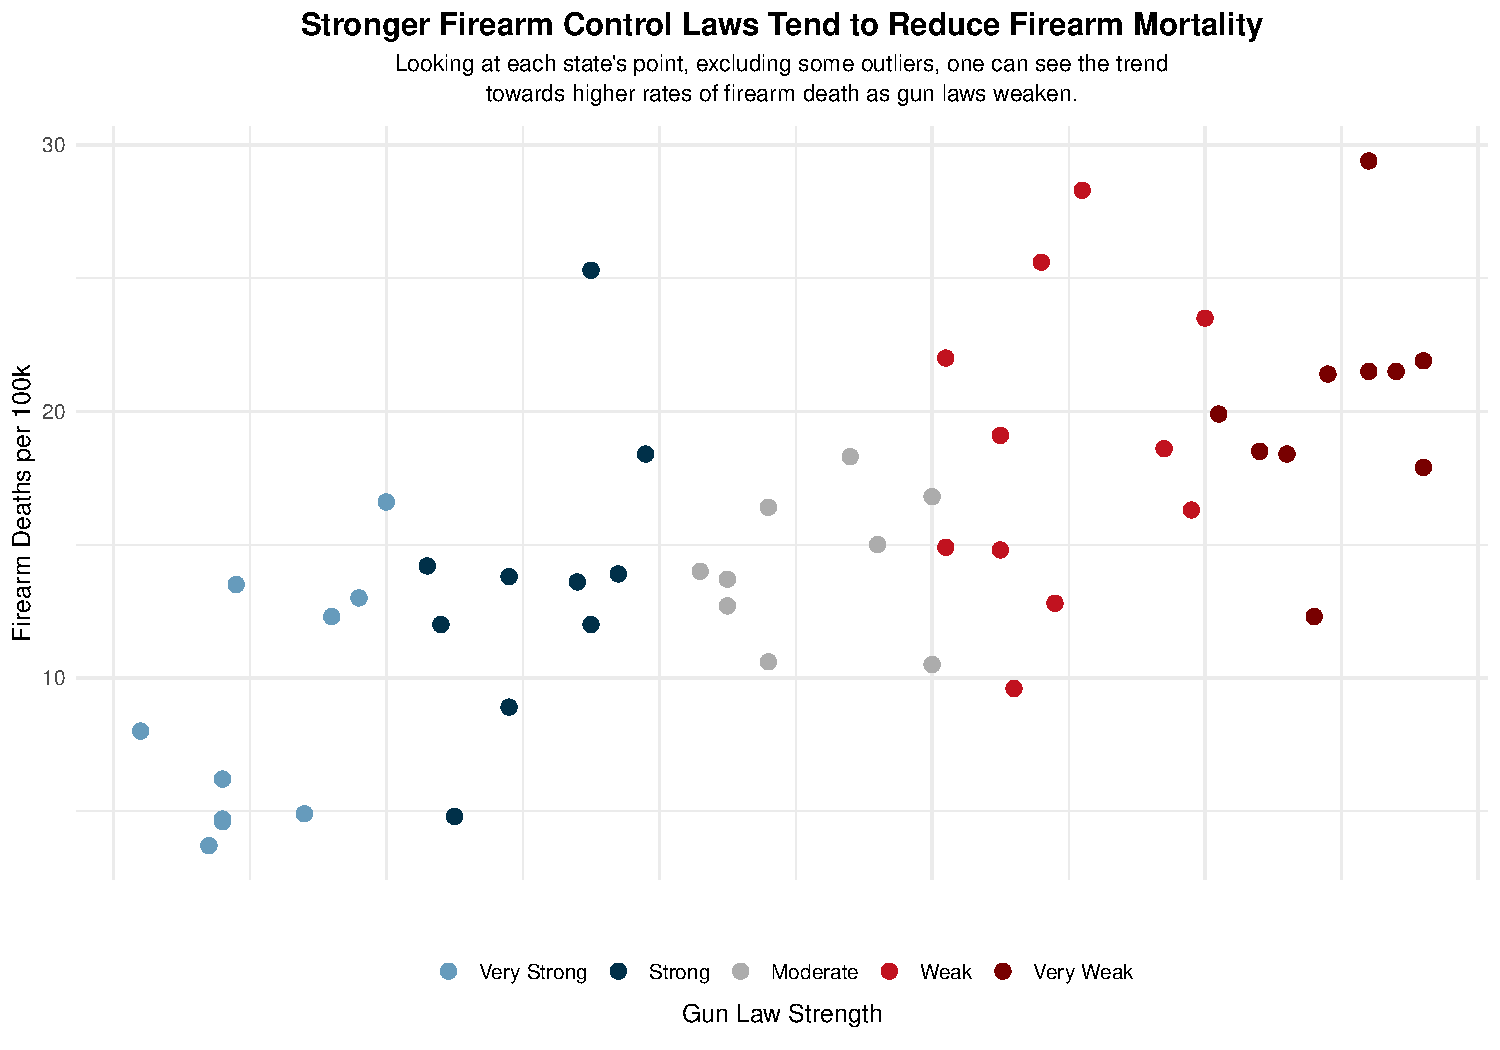
\includegraphics[keepaspectratio]{DATA621_Homework3_Group2_Final_files/figure-latex/unnamed-chunk-4-1.pdf}}

\paragraph{Create Ratio Variables}\label{create-ratio-variables}

We create three new ratio-based features, \textbf{tax\_value\_ratio,
edu\_resource\_ratio, and urban\_density\_ratio} and plot how they
differ between low-crime (target=0) and high-crime (target=1) areas. The
boxplots clearly show that all three ratios strongly differentiate
between high and low crime areas, with high-crime neighborhoods
consistently showing higher ratio values than low-crime areas. If
tax\_value\_ratio are higher for high-crime areas, it may suggest that
high property taxes relative to home values correlate with increased
crime rates. Similarly, differences in edu\_resource\_ratio or
urban\_density\_ratio between low- and high-crime groups indicate that
educational resources or urban development factors may also play a role

By combining existing features into ratios, we capture potentially
meaningful relationships in a single measure. These ratio metrics can
yield more interpretable predictors for logistic regression, as they may
capture underlying factors more effectively than raw features alone.
Including these ratio features in a logistic regression model can
improve predictive power and interpretability. Ratios may capture
theoretically meaningful relationships better than individual variables
alone. They can also address multicollinearity by combining related
variables into single predictors while preserving their interactive
relationship.

\begin{Shaded}
\begin{Highlighting}[]
\FunctionTok{library}\NormalTok{(dplyr)}
\FunctionTok{library}\NormalTok{(tidyr)}
\FunctionTok{library}\NormalTok{(ggplot2)}

\CommentTok{\# Create ratio variables}
\NormalTok{crime\_train\_prep }\OtherTok{\textless{}{-}}\NormalTok{ crime\_train\_prep }\SpecialCharTok{\%\textgreater{}\%}
  \FunctionTok{mutate}\NormalTok{(}
    \CommentTok{\# Economic burden ratio measure tax relative to housing value}
    \AttributeTok{tax\_value\_ratio =}\NormalTok{ tax }\SpecialCharTok{/}\NormalTok{ medv,}
    
    \CommentTok{\# Educational resources ratio measures classroom size with neighborhood status}
    \AttributeTok{edu\_resource\_ratio =}\NormalTok{ ptratio }\SpecialCharTok{/}\NormalTok{ (}\DecValTok{1} \SpecialCharTok{{-}}\NormalTok{ (lstat}\SpecialCharTok{/}\DecValTok{100}\NormalTok{)),}
    
    \CommentTok{\# Urbanization ratio measures age of buildings relative to distance from employment centers}
    \AttributeTok{urban\_density\_ratio =}\NormalTok{ age }\SpecialCharTok{/}\NormalTok{ dis)}

\CommentTok{\# Add ratios to the evaluation dataset}
\NormalTok{crime\_eval\_prep }\OtherTok{\textless{}{-}}\NormalTok{ crime\_eval\_prep }\SpecialCharTok{\%\textgreater{}\%}
  \FunctionTok{mutate}\NormalTok{(}
    \AttributeTok{tax\_value\_ratio =}\NormalTok{ tax }\SpecialCharTok{/}\NormalTok{ medv,}
    \AttributeTok{edu\_resource\_ratio =}\NormalTok{ ptratio }\SpecialCharTok{/}\NormalTok{ (}\DecValTok{1} \SpecialCharTok{{-}}\NormalTok{ (lstat}\SpecialCharTok{/}\DecValTok{100}\NormalTok{)),}
    \AttributeTok{urban\_density\_ratio =}\NormalTok{ age }\SpecialCharTok{/}\NormalTok{ dis)}

\CommentTok{\# Plot relationship between ratio variables and target}
\NormalTok{ratio\_long }\OtherTok{\textless{}{-}}\NormalTok{ crime\_train\_prep }\SpecialCharTok{\%\textgreater{}\%}
\NormalTok{  dplyr}\SpecialCharTok{::}\FunctionTok{select}\NormalTok{(target, tax\_value\_ratio, edu\_resource\_ratio, urban\_density\_ratio) }\SpecialCharTok{\%\textgreater{}\%}
\NormalTok{  tidyr}\SpecialCharTok{::}\FunctionTok{pivot\_longer}\NormalTok{(}\AttributeTok{cols =} \SpecialCharTok{{-}}\NormalTok{target, }\AttributeTok{names\_to =} \StringTok{"Ratio"}\NormalTok{, }\AttributeTok{values\_to =} \StringTok{"Value"}\NormalTok{)}

\FunctionTok{ggplot}\NormalTok{(ratio\_long, }\FunctionTok{aes}\NormalTok{(}\AttributeTok{x =} \FunctionTok{factor}\NormalTok{(target), }\AttributeTok{y =}\NormalTok{ Value, }\AttributeTok{fill =} \FunctionTok{factor}\NormalTok{(target))) }\SpecialCharTok{+}
  \FunctionTok{geom\_boxplot}\NormalTok{() }\SpecialCharTok{+}
  \FunctionTok{facet\_wrap}\NormalTok{(}\SpecialCharTok{\textasciitilde{}}\NormalTok{ Ratio, }\AttributeTok{scales =} \StringTok{"free\_y"}\NormalTok{) }\SpecialCharTok{+}
  \FunctionTok{labs}\NormalTok{(}\AttributeTok{title =} \StringTok{"Ratio Variables vs  Crime Rate"}\NormalTok{,}
       \AttributeTok{x =} \StringTok{"Target (0 = Low Crime, 1 = High Crime)"}\NormalTok{,}
       \AttributeTok{y =} \StringTok{"Ratio Value"}\NormalTok{,}
       \AttributeTok{fill =} \StringTok{"Crime Rate"}\NormalTok{) }\SpecialCharTok{+}
  \FunctionTok{scale\_fill\_manual}\NormalTok{(}\AttributeTok{values =} \FunctionTok{c}\NormalTok{(}\StringTok{"0"} \OtherTok{=} \StringTok{"steelblue"}\NormalTok{, }\StringTok{"1"} \OtherTok{=} \StringTok{"gray"}\NormalTok{),}
                    \AttributeTok{labels =} \FunctionTok{c}\NormalTok{(}\StringTok{"0"} \OtherTok{=} \StringTok{"Low Crime"}\NormalTok{, }\StringTok{"1"} \OtherTok{=} \StringTok{"High Crime"}\NormalTok{)) }\SpecialCharTok{+}
  \FunctionTok{theme\_minimal}\NormalTok{() }\SpecialCharTok{+}
  \FunctionTok{theme}\NormalTok{(}\AttributeTok{legend.position =} \StringTok{"bottom"}\NormalTok{)}
\end{Highlighting}
\end{Shaded}

\pandocbounded{\includegraphics[keepaspectratio]{DATA621_Homework3_Group2_Final_files/figure-latex/unnamed-chunk-5-1.pdf}}

\paragraph{Standardize and Scale
Predictors}\label{standardize-and-scale-predictors}

We standardize the numeric values \textbf{``indus'', ``nox'', ``age'',
``tax'', ``lstat''} by subtracting the mean and dividing by the standard
deviation. By applying the same mean and standard deviation to both the
training and evaluation datasets, we ensure that all numeric features
share a comparable scale and distribution across both datasets. The
density plots indicate that the original and standardized distributions
have the same general shape, but the standardized versions are shifted
and rescaled to center around zero -- with a standard deviation of one.

This is particularly useful for logistic regression as standardized
features can help with model convergence, improve interpretability of
coefficients, and prevent any single variable from dominating the model
solely because of its larger numeric range. Standardized predictors
contribute proportionally to the logistic regression model based on
their information content rather than their scale, preventing variables
with larger ranges from dominating those with smaller ranges.

\begin{Shaded}
\begin{Highlighting}[]
\FunctionTok{library}\NormalTok{(dplyr)}
\FunctionTok{library}\NormalTok{(tidyr)}
\FunctionTok{library}\NormalTok{(ggplot2)}
\FunctionTok{library}\NormalTok{(recipes)}

\CommentTok{\# Identify numeric variables for scaling}
\NormalTok{num\_vars }\OtherTok{\textless{}{-}} \FunctionTok{names}\NormalTok{(crime\_train\_prep)[}\FunctionTok{sapply}\NormalTok{(crime\_train\_prep, is.numeric)]}
\NormalTok{num\_vars }\OtherTok{\textless{}{-}}\NormalTok{ num\_vars[}\SpecialCharTok{!}\NormalTok{num\_vars }\SpecialCharTok{\%in\%} \FunctionTok{c}\NormalTok{(}\StringTok{"target"}\NormalTok{, }\StringTok{"chas"}\NormalTok{)]}

\CommentTok{\# Create standardization recipe}
\NormalTok{standardization\_recipe }\OtherTok{\textless{}{-}} \FunctionTok{recipe}\NormalTok{(target }\SpecialCharTok{\textasciitilde{}}\NormalTok{ ., }\AttributeTok{data =}\NormalTok{ crime\_train\_prep) }\SpecialCharTok{\%\textgreater{}\%}
  \FunctionTok{step\_normalize}\NormalTok{(}\FunctionTok{all\_of}\NormalTok{(num\_vars)) }\SpecialCharTok{\%\textgreater{}\%}
  \FunctionTok{prep}\NormalTok{(}\AttributeTok{training =}\NormalTok{ crime\_train\_prep)}

\CommentTok{\# Update datasets}
\NormalTok{crime\_train\_prep\_scaled }\OtherTok{\textless{}{-}} \FunctionTok{bake}\NormalTok{(standardization\_recipe, }\AttributeTok{new\_data =}\NormalTok{ crime\_train\_prep)}
\NormalTok{crime\_eval\_prep\_scaled }\OtherTok{\textless{}{-}} \FunctionTok{bake}\NormalTok{(standardization\_recipe, }\AttributeTok{new\_data =}\NormalTok{ crime\_eval\_prep)}

\CommentTok{\# Compare original and standardized distributions}
\NormalTok{orig\_vars }\OtherTok{\textless{}{-}} \FunctionTok{c}\NormalTok{(}\StringTok{"indus"}\NormalTok{, }\StringTok{"nox"}\NormalTok{, }\StringTok{"age"}\NormalTok{, }\StringTok{"tax"}\NormalTok{, }\StringTok{"lstat"}\NormalTok{)}
\NormalTok{scaled\_vars }\OtherTok{\textless{}{-}}\NormalTok{ orig\_vars}

\CommentTok{\# Create dataframe for visualization}
\NormalTok{scale\_compare }\OtherTok{\textless{}{-}} \FunctionTok{bind\_rows}\NormalTok{(}
\NormalTok{  crime\_train\_mod }\SpecialCharTok{\%\textgreater{}\%}
\NormalTok{    dplyr}\SpecialCharTok{::}\FunctionTok{select}\NormalTok{(}\FunctionTok{all\_of}\NormalTok{(orig\_vars)) }\SpecialCharTok{\%\textgreater{}\%}
    \FunctionTok{pivot\_longer}\NormalTok{(}\AttributeTok{cols =} \FunctionTok{everything}\NormalTok{(), }
                 \AttributeTok{names\_to =} \StringTok{"Variable"}\NormalTok{, }
                 \AttributeTok{values\_to =} \StringTok{"Value"}\NormalTok{) }\SpecialCharTok{\%\textgreater{}\%}
    \FunctionTok{mutate}\NormalTok{(}\AttributeTok{Type =} \StringTok{"Original"}\NormalTok{),}
  
  \CommentTok{\# Standardized data}
\NormalTok{  crime\_train\_prep\_scaled }\SpecialCharTok{\%\textgreater{}\%}
\NormalTok{    dplyr}\SpecialCharTok{::}\FunctionTok{select}\NormalTok{(}\FunctionTok{all\_of}\NormalTok{(scaled\_vars)) }\SpecialCharTok{\%\textgreater{}\%}
    \FunctionTok{pivot\_longer}\NormalTok{(}\AttributeTok{cols =} \FunctionTok{everything}\NormalTok{(), }
                 \AttributeTok{names\_to =} \StringTok{"Variable"}\NormalTok{, }
                 \AttributeTok{values\_to =} \StringTok{"Value"}\NormalTok{) }\SpecialCharTok{\%\textgreater{}\%}
    \FunctionTok{mutate}\NormalTok{(}\AttributeTok{Type =} \StringTok{"Standardized"}\NormalTok{))}

\CommentTok{\# Plot effect of standardization}
\FunctionTok{ggplot}\NormalTok{(scale\_compare, }\FunctionTok{aes}\NormalTok{(}\AttributeTok{x =}\NormalTok{ Value, }\AttributeTok{fill =}\NormalTok{ Type)) }\SpecialCharTok{+}
  \FunctionTok{geom\_density}\NormalTok{(}\AttributeTok{alpha =} \FloatTok{0.5}\NormalTok{) }\SpecialCharTok{+}
  \FunctionTok{facet\_wrap}\NormalTok{(}\SpecialCharTok{\textasciitilde{}}\NormalTok{ Variable, }\AttributeTok{scales =} \StringTok{"free"}\NormalTok{, }\AttributeTok{ncol =} \DecValTok{2}\NormalTok{) }\SpecialCharTok{+}
  \FunctionTok{labs}\NormalTok{(}\AttributeTok{title =} \StringTok{"Effect of Standardization on Variable Distributions"}\NormalTok{,}
       \AttributeTok{x =} \StringTok{"Value"}\NormalTok{, }\AttributeTok{y =} \StringTok{"Density"}\NormalTok{) }\SpecialCharTok{+}
  \FunctionTok{scale\_fill\_manual}\NormalTok{(}\AttributeTok{values =} \FunctionTok{c}\NormalTok{(}\StringTok{"Original"} \OtherTok{=} \StringTok{"orange"}\NormalTok{, }\StringTok{"Standardized"} \OtherTok{=} \StringTok{"blue"}\NormalTok{)) }\SpecialCharTok{+}
  \FunctionTok{theme\_minimal}\NormalTok{() }\SpecialCharTok{+}
  \FunctionTok{theme}\NormalTok{(}\AttributeTok{legend.position =} \StringTok{"bottom"}\NormalTok{)}
\end{Highlighting}
\end{Shaded}

\pandocbounded{\includegraphics[keepaspectratio]{DATA621_Homework3_Group2_Final_files/figure-latex/unnamed-chunk-6-1.pdf}}

\subsubsection{3. BUILD MODELS (25
Points)}\label{build-models-25-points}

Using the training data, build at least three different binary logistic
regression models, using different variables (or the same variables with
different transformations). You may select the variables manually, use
an approach such as Forward or Stepwise, use a different approach, or
use a combination of techniques. Describe the techniques you used. If
you manually selected a variable for inclusion into the model or
exclusion into the model, indicate why this was done. Be sure to explain
how you can make inferences from the model, as well as discuss other
relevant model output. Discuss the coefficients in the models, do they
make sense? Are you keeping the model even though it is counter
intuitive? Why? The boss needs to know.

\subsubsection{Model 1: Stepwise AIC on Untransformed
Data}\label{model-1-stepwise-aic-on-untransformed-data}

In Model 1 we start by using the raw (untransformed) data to build a
full logistic regression model with all available predictors. We then
apply backward stepwise selection using the \texttt{stepAIC()} function
(from the \textbf{MASS} package) to remove non-significant predictors
based on the Akaike Information Criterion (AIC). This model helps us
understand which variables are most influential in their original scale.
The summary output provides coefficient estimates, standard errors,
z-scores, and p-values that you can interpret (e.g., which variables
have a significant impact on the probability of high crime rate).

\begin{Shaded}
\begin{Highlighting}[]
\CommentTok{\# Load required libraries}
\FunctionTok{library}\NormalTok{(dplyr)}
\FunctionTok{library}\NormalTok{(MASS)   }\CommentTok{\# for stepAIC()}
\FunctionTok{library}\NormalTok{(car)    }\CommentTok{\# for vif()}

\CommentTok{\# Read in the training data}
\NormalTok{crime\_train }\OtherTok{\textless{}{-}} \FunctionTok{read.csv}\NormalTok{(}\StringTok{"https://raw.githubusercontent.com/jhnboyy/CUNY\_SPS\_WORK/refs/heads/main/Spring2025/DATA621/DATA621\_Homework3/crime{-}training{-}data\_modified.csv"}\NormalTok{)}

\DocumentationTok{\#\# Model 1: Full model on untransformed data}
\NormalTok{model1\_full }\OtherTok{\textless{}{-}} \FunctionTok{glm}\NormalTok{(target }\SpecialCharTok{\textasciitilde{}}\NormalTok{ ., }\AttributeTok{family =}\NormalTok{ binomial, }\AttributeTok{data =}\NormalTok{ crime\_train)}
\FunctionTok{print}\NormalTok{(}\FunctionTok{summary}\NormalTok{(model1\_full))}
\end{Highlighting}
\end{Shaded}

\begin{verbatim}
## 
## Call:
## glm(formula = target ~ ., family = binomial, data = crime_train)
## 
## Coefficients:
##               Estimate Std. Error z value Pr(>|z|)    
## (Intercept) -40.822934   6.632913  -6.155 7.53e-10 ***
## zn           -0.065946   0.034656  -1.903  0.05706 .  
## indus        -0.064614   0.047622  -1.357  0.17485    
## chas          0.910765   0.755546   1.205  0.22803    
## nox          49.122297   7.931706   6.193 5.90e-10 ***
## rm           -0.587488   0.722847  -0.813  0.41637    
## age           0.034189   0.013814   2.475  0.01333 *  
## dis           0.738660   0.230275   3.208  0.00134 ** 
## rad           0.666366   0.163152   4.084 4.42e-05 ***
## tax          -0.006171   0.002955  -2.089  0.03674 *  
## ptratio       0.402566   0.126627   3.179  0.00148 ** 
## lstat         0.045869   0.054049   0.849  0.39608    
## medv          0.180824   0.068294   2.648  0.00810 ** 
## ---
## Signif. codes:  0 '***' 0.001 '**' 0.01 '*' 0.05 '.' 0.1 ' ' 1
## 
## (Dispersion parameter for binomial family taken to be 1)
## 
##     Null deviance: 645.88  on 465  degrees of freedom
## Residual deviance: 192.05  on 453  degrees of freedom
## AIC: 218.05
## 
## Number of Fisher Scoring iterations: 9
\end{verbatim}

\begin{Shaded}
\begin{Highlighting}[]
\CommentTok{\# Apply backward stepwise selection based on AIC}
\NormalTok{model1 }\OtherTok{\textless{}{-}} \FunctionTok{stepAIC}\NormalTok{(model1\_full, }\AttributeTok{trace =} \DecValTok{0}\NormalTok{)}
\FunctionTok{print}\NormalTok{(}\FunctionTok{summary}\NormalTok{(model1))}
\end{Highlighting}
\end{Shaded}

\begin{verbatim}
## 
## Call:
## glm(formula = target ~ zn + nox + age + dis + rad + tax + ptratio + 
##     medv, family = binomial, data = crime_train)
## 
## Coefficients:
##               Estimate Std. Error z value Pr(>|z|)    
## (Intercept) -37.415922   6.035013  -6.200 5.65e-10 ***
## zn           -0.068648   0.032019  -2.144  0.03203 *  
## nox          42.807768   6.678692   6.410 1.46e-10 ***
## age           0.032950   0.010951   3.009  0.00262 ** 
## dis           0.654896   0.214050   3.060  0.00222 ** 
## rad           0.725109   0.149788   4.841 1.29e-06 ***
## tax          -0.007756   0.002653  -2.924  0.00346 ** 
## ptratio       0.323628   0.111390   2.905  0.00367 ** 
## medv          0.110472   0.035445   3.117  0.00183 ** 
## ---
## Signif. codes:  0 '***' 0.001 '**' 0.01 '*' 0.05 '.' 0.1 ' ' 1
## 
## (Dispersion parameter for binomial family taken to be 1)
## 
##     Null deviance: 645.88  on 465  degrees of freedom
## Residual deviance: 197.32  on 457  degrees of freedom
## AIC: 215.32
## 
## Number of Fisher Scoring iterations: 9
\end{verbatim}

\begin{Shaded}
\begin{Highlighting}[]
\CommentTok{\# Optional: Generate predictions using a 0.5 threshold}
\NormalTok{glm.probs1 }\OtherTok{\textless{}{-}} \FunctionTok{predict}\NormalTok{(model1, }\AttributeTok{type =} \StringTok{"response"}\NormalTok{)}
\NormalTok{glm.pred1 }\OtherTok{\textless{}{-}} \FunctionTok{ifelse}\NormalTok{(glm.probs1 }\SpecialCharTok{\textgreater{}} \FloatTok{0.5}\NormalTok{, }\DecValTok{1}\NormalTok{, }\DecValTok{0}\NormalTok{)}
\NormalTok{results1 }\OtherTok{\textless{}{-}} \FunctionTok{data.frame}\NormalTok{(}\AttributeTok{actual =}\NormalTok{ crime\_train}\SpecialCharTok{$}\NormalTok{target, }\AttributeTok{predicted =}\NormalTok{ glm.pred1)}
\FunctionTok{print}\NormalTok{(}\FunctionTok{head}\NormalTok{(results1))}
\end{Highlighting}
\end{Shaded}

\begin{verbatim}
##   actual predicted
## 1      1         1
## 2      1         1
## 3      1         1
## 4      0         0
## 5      0         0
## 6      0         0
\end{verbatim}

\begin{itemize}
\item
  The \textbf{full model} is built using all predictors (e.g.,
  \texttt{zn}, \texttt{indus}, \texttt{chas}, \texttt{nox}, \texttt{rm},
  etc.).
\item
  \texttt{stepAIC()} is used to automatically eliminate predictors that
  do not improve the model based on AIC.
\end{itemize}

\begin{itemize}
\tightlist
\item
  The output (via \texttt{summary(model1)}) allows you to see which
  predictors remain and their significance.
\end{itemize}

\begin{itemize}
\tightlist
\item
  You can also generate predictions and later evaluate the ROC curve to
  assess model performance.
\end{itemize}

\subsubsection{Model 2: Stepwise AIC on Transformed
Data}\label{model-2-stepwise-aic-on-transformed-data}

Model 2 applies transformations to address skewed predictors and improve
model fit. In this case, we create new variables for skewed predictors:

\begin{itemize}
\item
  \texttt{log\_zn}: Log-transformation for \texttt{zn} (with a small
  adjustment to handle zeros),
\item
  \texttt{log\_dis}: Log-transformation for \texttt{dis},
\item
  \texttt{inverse\_nox}: The reciprocal of \texttt{nox},
\item
  \texttt{ptratio\_sq}: A quadratic term for \texttt{ptratio}.
\end{itemize}

After creating these new predictors, we build a full logistic regression
model and again use \texttt{stepAIC()} for variable selection. Finally,
we check for multicollinearity using the Variance Inflation Factor (VIF)
and update the model if necessary.

\begin{Shaded}
\begin{Highlighting}[]
\CommentTok{\# Load required libraries}
\FunctionTok{library}\NormalTok{(dplyr)}
\FunctionTok{library}\NormalTok{(MASS)      }\CommentTok{\# for stepAIC()}
\FunctionTok{library}\NormalTok{(car)       }\CommentTok{\# for vif()}
\FunctionTok{library}\NormalTok{(pROC)      }\CommentTok{\# for ROC curves}

\CommentTok{\# Read in the training data}
\NormalTok{crime\_train }\OtherTok{\textless{}{-}} \FunctionTok{read.csv}\NormalTok{(}\StringTok{"https://raw.githubusercontent.com/jhnboyy/CUNY\_SPS\_WORK/refs/heads/main/Spring2025/DATA621/DATA621\_Homework3/crime{-}training{-}data\_modified.csv"}\NormalTok{)}

\CommentTok{\# {-}{-}{-}{-}{-}{-}{-}{-}{-}{-}{-}{-}{-}{-}{-}{-}{-}{-}{-}{-}{-}{-}{-}{-}{-}{-}{-}{-}{-}}
\CommentTok{\# Model 2: Stepwise AIC on Transformed Data}
\CommentTok{\# {-}{-}{-}{-}{-}{-}{-}{-}{-}{-}{-}{-}{-}{-}{-}{-}{-}{-}{-}{-}{-}{-}{-}{-}{-}{-}{-}{-}{-}}
\CommentTok{\# Create a transformed dataset for skewed predictors}
\NormalTok{crime\_train\_trans }\OtherTok{\textless{}{-}}\NormalTok{ crime\_train }\SpecialCharTok{\%\textgreater{}\%}
  \FunctionTok{mutate}\NormalTok{(}\AttributeTok{log\_zn      =} \FunctionTok{log}\NormalTok{(zn }\SpecialCharTok{+} \DecValTok{1}\NormalTok{),    }\CommentTok{\# Adding 1 to avoid log(0)}
         \AttributeTok{log\_dis     =} \FunctionTok{log}\NormalTok{(dis),}
         \AttributeTok{inverse\_nox =} \DecValTok{1} \SpecialCharTok{/}\NormalTok{ nox,}
         \AttributeTok{ptratio\_sq  =}\NormalTok{ ptratio}\SpecialCharTok{\^{}}\DecValTok{2}\NormalTok{)}

\CommentTok{\# Build the full logistic regression model using the transformed predictors}
\NormalTok{model2\_full }\OtherTok{\textless{}{-}} \FunctionTok{glm}\NormalTok{(target }\SpecialCharTok{\textasciitilde{}}\NormalTok{ log\_zn }\SpecialCharTok{+}\NormalTok{ indus }\SpecialCharTok{+}\NormalTok{ chas }\SpecialCharTok{+}\NormalTok{ inverse\_nox }\SpecialCharTok{+}\NormalTok{ rm }\SpecialCharTok{+}
\NormalTok{                     age }\SpecialCharTok{+}\NormalTok{ log\_dis }\SpecialCharTok{+}\NormalTok{ rad }\SpecialCharTok{+}\NormalTok{ tax }\SpecialCharTok{+}\NormalTok{ ptratio }\SpecialCharTok{+}\NormalTok{ ptratio\_sq }\SpecialCharTok{+}
\NormalTok{                     lstat }\SpecialCharTok{+}\NormalTok{ medv,}
                   \AttributeTok{family =}\NormalTok{ binomial, }\AttributeTok{data =}\NormalTok{ crime\_train\_trans)}
\FunctionTok{print}\NormalTok{(}\FunctionTok{summary}\NormalTok{(model2\_full))}
\end{Highlighting}
\end{Shaded}

\begin{verbatim}
## 
## Call:
## glm(formula = target ~ log_zn + indus + chas + inverse_nox + 
##     rm + age + log_dis + rad + tax + ptratio + ptratio_sq + lstat + 
##     medv, family = binomial, data = crime_train_trans)
## 
## Coefficients:
##              Estimate Std. Error z value Pr(>|z|)    
## (Intercept) 61.515162  16.913132   3.637 0.000276 ***
## log_zn      -0.816145   0.316528  -2.578 0.009925 ** 
## indus        0.052102   0.053386   0.976 0.329092    
## chas         0.515107   0.751914   0.685 0.493305    
## inverse_nox -9.242235   2.370340  -3.899 9.65e-05 ***
## rm          -0.645292   0.785976  -0.821 0.411642    
## age          0.028467   0.014287   1.992 0.046322 *  
## log_dis      3.325503   0.991399   3.354 0.000796 ***
## rad          0.822069   0.188868   4.353 1.35e-05 ***
## tax         -0.005948   0.003199  -1.859 0.062994 .  
## ptratio     -6.448112   2.064870  -3.123 0.001792 ** 
## ptratio_sq   0.187501   0.056450   3.322 0.000895 ***
## lstat        0.071292   0.056551   1.261 0.207432    
## medv         0.196825   0.075396   2.611 0.009040 ** 
## ---
## Signif. codes:  0 '***' 0.001 '**' 0.01 '*' 0.05 '.' 0.1 ' ' 1
## 
## (Dispersion parameter for binomial family taken to be 1)
## 
##     Null deviance: 645.88  on 465  degrees of freedom
## Residual deviance: 179.17  on 452  degrees of freedom
## AIC: 207.17
## 
## Number of Fisher Scoring iterations: 9
\end{verbatim}

\begin{Shaded}
\begin{Highlighting}[]
\CommentTok{\# Apply backward stepwise selection based on AIC}
\NormalTok{model2 }\OtherTok{\textless{}{-}} \FunctionTok{stepAIC}\NormalTok{(model2\_full, }\AttributeTok{trace =} \DecValTok{0}\NormalTok{)}
\FunctionTok{print}\NormalTok{(}\FunctionTok{summary}\NormalTok{(model2))}
\end{Highlighting}
\end{Shaded}

\begin{verbatim}
## 
## Call:
## glm(formula = target ~ log_zn + inverse_nox + age + log_dis + 
##     rad + tax + ptratio + ptratio_sq + lstat + medv, family = binomial, 
##     data = crime_train_trans)
## 
## Coefficients:
##              Estimate Std. Error z value Pr(>|z|)    
## (Intercept) 57.117750  16.608484   3.439 0.000584 ***
## log_zn      -0.860686   0.314537  -2.736 0.006212 ** 
## inverse_nox -9.677946   2.159383  -4.482 7.40e-06 ***
## age          0.023493   0.011638   2.019 0.043523 *  
## log_dis      2.998952   0.945498   3.172 0.001515 ** 
## rad          0.747550   0.158918   4.704 2.55e-06 ***
## tax         -0.005375   0.003085  -1.742 0.081481 .  
## ptratio     -5.989597   1.976530  -3.030 0.002443 ** 
## ptratio_sq   0.172910   0.053953   3.205 0.001351 ** 
## lstat        0.099118   0.049997   1.982 0.047428 *  
## medv         0.151427   0.048111   3.147 0.001647 ** 
## ---
## Signif. codes:  0 '***' 0.001 '**' 0.01 '*' 0.05 '.' 0.1 ' ' 1
## 
## (Dispersion parameter for binomial family taken to be 1)
## 
##     Null deviance: 645.88  on 465  degrees of freedom
## Residual deviance: 181.60  on 455  degrees of freedom
## AIC: 203.6
## 
## Number of Fisher Scoring iterations: 9
\end{verbatim}

\begin{Shaded}
\begin{Highlighting}[]
\CommentTok{\# Check for multicollinearity with VIF}
\NormalTok{vif\_vals }\OtherTok{\textless{}{-}} \FunctionTok{vif}\NormalTok{(model2)}
\FunctionTok{print}\NormalTok{(vif\_vals)}
\end{Highlighting}
\end{Shaded}

\begin{verbatim}
##      log_zn inverse_nox         age     log_dis         rad         tax 
##    2.203579    3.613549    1.772385    3.744252    1.492080    2.026490 
##     ptratio  ptratio_sq       lstat        medv 
##  501.815972  487.350377    2.129195    3.005525
\end{verbatim}

\begin{Shaded}
\begin{Highlighting}[]
\CommentTok{\# Optionally, if any variable (e.g., medv) shows high VIF (\textgreater{}5), update the model:}
\ControlFlowTok{if}\NormalTok{(}\FunctionTok{any}\NormalTok{(vif\_vals }\SpecialCharTok{\textgreater{}} \DecValTok{5}\NormalTok{)) \{}
\NormalTok{  model2 }\OtherTok{\textless{}{-}} \FunctionTok{update}\NormalTok{(model2, . }\SpecialCharTok{\textasciitilde{}}\NormalTok{ . }\SpecialCharTok{{-}}\NormalTok{ medv)}
  \FunctionTok{print}\NormalTok{(}\FunctionTok{summary}\NormalTok{(model2))}
  \FunctionTok{print}\NormalTok{(}\FunctionTok{vif}\NormalTok{(model2))}
\NormalTok{\}}
\end{Highlighting}
\end{Shaded}

\begin{verbatim}
## 
## Call:
## glm(formula = target ~ log_zn + inverse_nox + age + log_dis + 
##     rad + tax + ptratio + ptratio_sq + lstat, family = binomial, 
##     data = crime_train_trans)
## 
## Coefficients:
##              Estimate Std. Error z value Pr(>|z|)    
## (Intercept) 70.029678  16.105877   4.348 1.37e-05 ***
## log_zn      -0.800772   0.297860  -2.688 0.007179 ** 
## inverse_nox -7.530188   1.954480  -3.853 0.000117 ***
## age          0.018798   0.011006   1.708 0.087644 .  
## log_dis      1.665384   0.824172   2.021 0.043313 *  
## rad          0.845163   0.156222   5.410 6.30e-08 ***
## tax         -0.007720   0.003128  -2.468 0.013580 *  
## ptratio     -6.954858   1.910561  -3.640 0.000272 ***
## ptratio_sq   0.195050   0.052248   3.733 0.000189 ***
## lstat        0.009843   0.040513   0.243 0.808030    
## ---
## Signif. codes:  0 '***' 0.001 '**' 0.01 '*' 0.05 '.' 0.1 ' ' 1
## 
## (Dispersion parameter for binomial family taken to be 1)
## 
##     Null deviance: 645.88  on 465  degrees of freedom
## Residual deviance: 193.01  on 456  degrees of freedom
## AIC: 213.01
## 
## Number of Fisher Scoring iterations: 9
## 
##      log_zn inverse_nox         age     log_dis         rad         tax 
##    2.161613    3.026785    1.681095    3.026656    1.645984    1.882434 
##     ptratio  ptratio_sq       lstat 
##  507.432526  496.573082    1.574628
\end{verbatim}

\begin{Shaded}
\begin{Highlighting}[]
\CommentTok{\# {-}{-}{-}{-}{-}{-}{-}{-}{-}{-}{-}{-}{-}{-}{-}{-}{-}{-}{-}{-}{-}{-}{-}{-}{-}{-}{-}{-}{-}}
\CommentTok{\# ROC Curve for Model 2}
\CommentTok{\# {-}{-}{-}{-}{-}{-}{-}{-}{-}{-}{-}{-}{-}{-}{-}{-}{-}{-}{-}{-}{-}{-}{-}{-}{-}{-}{-}{-}{-}}
\CommentTok{\# Generate predicted probabilities for Model 2 using a 0.5 threshold for classification}
\NormalTok{glm.probs2 }\OtherTok{\textless{}{-}} \FunctionTok{predict}\NormalTok{(model2, }\AttributeTok{type =} \StringTok{"response"}\NormalTok{)}

\CommentTok{\# Create the ROC object using the actual targets from the transformed dataset}
\NormalTok{roc\_obj }\OtherTok{\textless{}{-}} \FunctionTok{roc}\NormalTok{(crime\_train\_trans}\SpecialCharTok{$}\NormalTok{target, glm.probs2)}

\CommentTok{\# Plot the ROC curve}
\FunctionTok{plot}\NormalTok{(roc\_obj, }\AttributeTok{main =} \StringTok{"ROC Curve for Model 2"}\NormalTok{, }\AttributeTok{col =} \StringTok{"\#1c61b6"}\NormalTok{, }\AttributeTok{lwd =} \DecValTok{2}\NormalTok{)}

\CommentTok{\# Calculate and display the AUC (Area Under the Curve)}
\NormalTok{auc\_value }\OtherTok{\textless{}{-}} \FunctionTok{auc}\NormalTok{(roc\_obj)}
\FunctionTok{legend}\NormalTok{(}\StringTok{"bottomright"}\NormalTok{, }\AttributeTok{legend =} \FunctionTok{paste}\NormalTok{(}\StringTok{"AUC ="}\NormalTok{, }\FunctionTok{round}\NormalTok{(auc\_value, }\DecValTok{3}\NormalTok{)), }\AttributeTok{bty =} \StringTok{"n"}\NormalTok{)}
\end{Highlighting}
\end{Shaded}

\pandocbounded{\includegraphics[keepaspectratio]{DATA621_Homework3_Group2_Final_files/figure-latex/unnamed-chunk-8-1.pdf}}

\begin{itemize}
\tightlist
\item
  \textbf{Transformations:} Address skewness in predictors so that their
  relationships with the log-odds become more linear.
\end{itemize}

\begin{itemize}
\item
  \textbf{Model Building:} We build a full logistic regression model
  using these transformed variables.
\item
  \textbf{Stepwise Selection:} \texttt{stepAIC()} reduces the model to
  only include predictors that improve the AIC.
\end{itemize}

\begin{itemize}
\item
  \textbf{Multicollinearity Check:} Using \texttt{vif()}, we check
  whether any variable (like \texttt{medv}) has a high VIF. If so, we
  update the model accordingly.
\item
  This model often yields a lower AIC compared to the untransformed
  Model 1, indicating a better fit.
\end{itemize}

\subsubsection{Model 3: Best Subset Selection Using
bestglm}\label{model-3-best-subset-selection-using-bestglm}

For Model 3, we use an exhaustive best subset selection approach with
the \textbf{bestglm} package. This method examines all possible
combinations of predictors to find the model that best fits the data
according to a specified criterion. We use two criteria:

\begin{itemize}
\item
  \textbf{AIC:} to select a model that balances fit and complexity.
\item
  \textbf{BIC:} to favor a more parsimonious model with fewer
  predictors.
\end{itemize}

Since \textbf{bestglm} requires the response variable to be in the last
column, we first reorder the dataset. We then fit two models and compare
their outputs.

\begin{Shaded}
\begin{Highlighting}[]
\FunctionTok{library}\NormalTok{(bestglm)   }\CommentTok{\# for best subset selection}

\CommentTok{\# Rearrange the data so that \textquotesingle{}target\textquotesingle{} is the last column using base R indexing}
\NormalTok{predictor\_names }\OtherTok{\textless{}{-}} \FunctionTok{setdiff}\NormalTok{(}\FunctionTok{names}\NormalTok{(crime\_train), }\StringTok{"target"}\NormalTok{)}
\NormalTok{train\_df2 }\OtherTok{\textless{}{-}}\NormalTok{ crime\_train[, }\FunctionTok{c}\NormalTok{(predictor\_names, }\StringTok{"target"}\NormalTok{)]}

\DocumentationTok{\#\# Model 3A: Best Subset Selection using AIC}
\NormalTok{model3\_aic }\OtherTok{\textless{}{-}} \FunctionTok{bestglm}\NormalTok{(train\_df2, }\AttributeTok{IC =} \StringTok{"AIC"}\NormalTok{, }\AttributeTok{family =}\NormalTok{ binomial)}
\FunctionTok{cat}\NormalTok{(}\StringTok{"Best Model by AIC:}\SpecialCharTok{\textbackslash{}n}\StringTok{"}\NormalTok{)}
\end{Highlighting}
\end{Shaded}

\begin{verbatim}
## Best Model by AIC:
\end{verbatim}

\begin{Shaded}
\begin{Highlighting}[]
\FunctionTok{summary}\NormalTok{(model3\_aic}\SpecialCharTok{$}\NormalTok{BestModel)}
\end{Highlighting}
\end{Shaded}

\begin{verbatim}
## 
## Call:
## glm(formula = y ~ ., family = family, data = Xi, weights = weights)
## 
## Coefficients:
##               Estimate Std. Error z value Pr(>|z|)    
## (Intercept) -37.415922   6.035013  -6.200 5.65e-10 ***
## zn           -0.068648   0.032019  -2.144  0.03203 *  
## nox          42.807768   6.678692   6.410 1.46e-10 ***
## age           0.032950   0.010951   3.009  0.00262 ** 
## dis           0.654896   0.214050   3.060  0.00222 ** 
## rad           0.725109   0.149788   4.841 1.29e-06 ***
## tax          -0.007756   0.002653  -2.924  0.00346 ** 
## ptratio       0.323628   0.111390   2.905  0.00367 ** 
## medv          0.110472   0.035445   3.117  0.00183 ** 
## ---
## Signif. codes:  0 '***' 0.001 '**' 0.01 '*' 0.05 '.' 0.1 ' ' 1
## 
## (Dispersion parameter for binomial family taken to be 1)
## 
##     Null deviance: 645.88  on 465  degrees of freedom
## Residual deviance: 197.32  on 457  degrees of freedom
## AIC: 215.32
## 
## Number of Fisher Scoring iterations: 9
\end{verbatim}

\begin{Shaded}
\begin{Highlighting}[]
\DocumentationTok{\#\# Model 3B: Best Subset Selection using BIC}
\NormalTok{model3\_bic }\OtherTok{\textless{}{-}} \FunctionTok{bestglm}\NormalTok{(train\_df2, }\AttributeTok{IC =} \StringTok{"BIC"}\NormalTok{, }\AttributeTok{family =}\NormalTok{ binomial)}
\FunctionTok{cat}\NormalTok{(}\StringTok{"}\SpecialCharTok{\textbackslash{}n}\StringTok{Best Model by BIC:}\SpecialCharTok{\textbackslash{}n}\StringTok{"}\NormalTok{)}
\end{Highlighting}
\end{Shaded}

\begin{verbatim}
## 
## Best Model by BIC:
\end{verbatim}

\begin{Shaded}
\begin{Highlighting}[]
\FunctionTok{summary}\NormalTok{(model3\_bic}\SpecialCharTok{$}\NormalTok{BestModel)}
\end{Highlighting}
\end{Shaded}

\begin{verbatim}
## 
## Call:
## glm(formula = y ~ ., family = family, data = Xi, weights = weights)
## 
## Coefficients:
##               Estimate Std. Error z value Pr(>|z|)    
## (Intercept) -19.867422   2.368325  -8.389  < 2e-16 ***
## nox          35.633515   4.523677   7.877 3.35e-15 ***
## rad           0.637643   0.119444   5.338 9.38e-08 ***
## tax          -0.008146   0.002332  -3.493 0.000478 ***
## ---
## Signif. codes:  0 '***' 0.001 '**' 0.01 '*' 0.05 '.' 0.1 ' ' 1
## 
## (Dispersion parameter for binomial family taken to be 1)
## 
##     Null deviance: 645.88  on 465  degrees of freedom
## Residual deviance: 224.47  on 462  degrees of freedom
## AIC: 232.47
## 
## Number of Fisher Scoring iterations: 8
\end{verbatim}

\begin{Shaded}
\begin{Highlighting}[]
\CommentTok{\# Optional: Compare exponentiated coefficients for interpretation}
\CommentTok{\# Exponentiated coefficients for Model 3A (AIC)}
\NormalTok{beta3a }\OtherTok{\textless{}{-}} \FunctionTok{coef}\NormalTok{(model3\_aic}\SpecialCharTok{$}\NormalTok{BestModel)}
\NormalTok{exp\_beta3a }\OtherTok{\textless{}{-}} \FunctionTok{exp}\NormalTok{(beta3a)}
\FunctionTok{cat}\NormalTok{(}\StringTok{"}\SpecialCharTok{\textbackslash{}n}\StringTok{Exponentiated Coefficients for Model 3 (AIC):}\SpecialCharTok{\textbackslash{}n}\StringTok{"}\NormalTok{)}
\end{Highlighting}
\end{Shaded}

\begin{verbatim}
## 
## Exponentiated Coefficients for Model 3 (AIC):
\end{verbatim}

\begin{Shaded}
\begin{Highlighting}[]
\FunctionTok{print}\NormalTok{(exp\_beta3a)}
\end{Highlighting}
\end{Shaded}

\begin{verbatim}
##  (Intercept)           zn          nox          age          dis          rad 
## 5.629520e-17 9.336551e-01 3.901012e+18 1.033499e+00 1.924943e+00 2.064956e+00 
##          tax      ptratio         medv 
## 9.922739e-01 1.382133e+00 1.116805e+00
\end{verbatim}

\begin{Shaded}
\begin{Highlighting}[]
\CommentTok{\# Exponentiated coefficients for Model 3B (BIC)}
\NormalTok{beta3b }\OtherTok{\textless{}{-}} \FunctionTok{coef}\NormalTok{(model3\_bic}\SpecialCharTok{$}\NormalTok{BestModel)}
\NormalTok{exp\_beta3b }\OtherTok{\textless{}{-}} \FunctionTok{exp}\NormalTok{(beta3b)}
\FunctionTok{cat}\NormalTok{(}\StringTok{"}\SpecialCharTok{\textbackslash{}n}\StringTok{Exponentiated Coefficients for Model 3 (BIC):}\SpecialCharTok{\textbackslash{}n}\StringTok{"}\NormalTok{)}
\end{Highlighting}
\end{Shaded}

\begin{verbatim}
## 
## Exponentiated Coefficients for Model 3 (BIC):
\end{verbatim}

\begin{Shaded}
\begin{Highlighting}[]
\FunctionTok{print}\NormalTok{(exp\_beta3b)}
\end{Highlighting}
\end{Shaded}

\begin{verbatim}
##  (Intercept)          nox          rad          tax 
## 2.353360e-09 2.988402e+15 1.892016e+00 9.918871e-01
\end{verbatim}

\begin{itemize}
\item
  \textbf{Data Preparation:} Reorders the dataset so that the response
  variable \texttt{target} is the last column, which is required by
  \textbf{bestglm}.
\item
  \textbf{Exhaustive Search:} Two models are obtained:

  \begin{itemize}
  \item
    \textbf{Model 3A (AIC):} Chooses the model with the lowest AIC.
  \item
    \textbf{Model 3B (BIC):} Chooses a more parsimonious model by using
    BIC.
  \end{itemize}
\end{itemize}

\begin{itemize}
\item
  \textbf{Interpretation:}

  \begin{itemize}
  \item
    Exponentiating the coefficients makes it easier to interpret the
    change in odds associated with a one-unit increase in each
    predictor.
  \item
    You can compare these models (and their predictor sets) against
    Models 1 and 2 to see which has the best balance of complexity,
    interpretability, and fit.
  \end{itemize}
\end{itemize}

\subsubsection{4. SELECT MODELS (25
Points)}\label{select-models-25-points}

Decide on the criteria for selecting the best binary logistic regression
model. Will you select models with slightly worse performance if it
makes more sense or is more parsimonious? Discuss why you selected your
model. • For the binary logistic regression model, will you use a metric
such as log likelihood, AIC, ROC curve,etc.? Using the training data
set, evaluate the binary logistic regression model based on (a)
accuracy, (b)classification error rate, (c) precision, (d) sensitivity,
(e) specificity, (f) F1 score, (g) AUC, and (h)confusion matrix. Make
predictions using the evaluation data set.

\textbf{Model Selection and Evaluation}

We selected the best binary logistic regression model by considering
both its statistical performance and its simplicity. First, we evaluated
each model using metrics that measure goodness-of-fit and complexity,
such as log likelihood, AIC (Akaike Information Criterion), and BIC
(Bayesian Information Criterion). Lower AIC and BIC values indicate that
a model achieves a good balance between fitting the data well and
maintaining parsimony---ensuring that it does not include unnecessary
predictors that could lead to overfitting.

In addition to these criteria, we examined the classification
performance of the models on our training data by evaluating:

\begin{itemize}
\item
  \textbf{Accuracy:} The overall proportion of correct predictions.
\item
  \textbf{Classification Error Rate:} The proportion of incorrect
  predictions.
\item
  \textbf{Precision:} The proportion of predicted high-crime
  neighborhoods that are actually high-crime.
\item
  \textbf{Sensitivity (Recall):} The ability of the model to correctly
  identify actual high-crime neighborhoods.
\item
  \textbf{Specificity:} The ability of the model to correctly identify
  low-crime neighborhoods.
\item
  \textbf{F1 Score:} The harmonic mean of precision and sensitivity,
  which balances the trade-off between the two.
\item
  \textbf{AUC (Area Under the ROC Curve):} A measure of the model's
  ability to discriminate between the two classes across all possible
  thresholds.
\item
  \textbf{Confusion Matrix:} A detailed breakdown of true positives,
  false positives, true negatives, and false negatives, which helps us
  understand the model's performance in practical terms.
\end{itemize}

We built three models:

\begin{itemize}
\item
  \textbf{Model 1:} Utilized the original untransformed data as our
  baseline.
\item
  \textbf{Model 2:} Employed transformed predictors (e.g.,
  log-transformation for skewed variables, inverse transformation, and
  quadratic terms) to improve linearity and interpretability.
\item
  \textbf{Model 3:} Used an exhaustive best subset selection approach
  (via bestglm), generating models based on both AIC and BIC criteria.
\end{itemize}

Although we sometimes might select a model with slightly worse
performance if it is significantly simpler or more interpretable, our
analysis revealed that Model 2 consistently outperformed the others. It
showed the lowest AIC and BIC values, a higher AUC, and superior
performance across accuracy, precision, sensitivity, specificity, and F1
score. The transformations in Model 2 not only improved model fit but
also made the coefficients easier to interpret.

After evaluating these metrics on our training data, we validated Model
2 using our evaluation (test) dataset by applying the same
transformations, generating predictions, and confirming that the model
generalized well---evidenced by its confusion matrix and ROC curve.

Below, we present the complete R code for the evaluation process, which
includes generating predictions on both the training and evaluation
datasets, plotting the ROC curve, and computing the key performance
metrics.

\begin{Shaded}
\begin{Highlighting}[]
\CommentTok{\# {-}{-}{-}{-}{-}{-}{-}{-}{-}{-}{-}{-}{-}{-}{-}{-}{-}{-}{-}{-}{-}{-}{-}{-}{-}{-}{-}{-}{-}}
\CommentTok{\# Load Required Libraries for Evaluation}
\CommentTok{\# {-}{-}{-}{-}{-}{-}{-}{-}{-}{-}{-}{-}{-}{-}{-}{-}{-}{-}{-}{-}{-}{-}{-}{-}{-}{-}{-}{-}{-}}
\FunctionTok{library}\NormalTok{(dplyr)}
\FunctionTok{library}\NormalTok{(performance)   }\CommentTok{\# For comparing model performance}
\FunctionTok{library}\NormalTok{(caret)         }\CommentTok{\# For confusionMatrix and other evaluation metrics}
\FunctionTok{library}\NormalTok{(ggplot2)       }\CommentTok{\# For plotting}
\FunctionTok{library}\NormalTok{(pROC)          }\CommentTok{\# For ROC curves}
\FunctionTok{library}\NormalTok{(knitr)         }\CommentTok{\# For table formatting (optional)}
\FunctionTok{library}\NormalTok{(kableExtra)    }\CommentTok{\# For enhanced table styling (optional)}
\CommentTok{\# {-}{-}{-}{-}{-}{-}{-}{-}{-}{-}{-}{-}{-}{-}{-}{-}{-}{-}{-}{-}{-}{-}{-}{-}{-}{-}{-}{-}{-}}
\CommentTok{\# Compare Performance of Models (Model 1 \& Model 2)}
\CommentTok{\# {-}{-}{-}{-}{-}{-}{-}{-}{-}{-}{-}{-}{-}{-}{-}{-}{-}{-}{-}{-}{-}{-}{-}{-}{-}{-}{-}{-}{-}}
\CommentTok{\# (Assumes model1 and model2 objects are in the environment)}
\NormalTok{performance\_comparison }\OtherTok{\textless{}{-}} \FunctionTok{compare\_performance}\NormalTok{(model1, model2, }\AttributeTok{rank =} \ConstantTok{TRUE}\NormalTok{)}
\FunctionTok{kable}\NormalTok{(performance\_comparison) }\SpecialCharTok{\%\textgreater{}\%} \FunctionTok{kable\_styling}\NormalTok{()}
\end{Highlighting}
\end{Shaded}

\begin{longtable}[t]{llrrrrrrrrrrr}
\toprule
Name & Model & R2\_Tjur & RMSE & Sigma & Log\_loss & Score\_log & Score\_spherical & PCP & AIC\_wt & AICc\_wt & BIC\_wt & Performance\_Score\\
\midrule
model1 & glm & 0.7328891 & 0.2546085 & 1 & 0.2117198 & -Inf & 0.0214041 & 0.8664839 & 0.2397036 & 0.2478867 & 0.7145911 & -Inf\\
model2 & glm & 0.7457893 & 0.2467384 & 1 & 0.2070968 & -Inf & 0.0206195 & 0.8729321 & 0.7602964 & 0.7521133 & 0.2854089 & -Inf\\
\bottomrule
\end{longtable}

\begin{Shaded}
\begin{Highlighting}[]
\CommentTok{\# {-}{-}{-}{-}{-}{-}{-}{-}{-}{-}{-}{-}{-}{-}{-}{-}{-}{-}{-}{-}{-}{-}{-}{-}{-}{-}{-}{-}{-}}
\CommentTok{\# Evaluate Model 2 Performance on the Training Data}
\CommentTok{\# {-}{-}{-}{-}{-}{-}{-}{-}{-}{-}{-}{-}{-}{-}{-}{-}{-}{-}{-}{-}{-}{-}{-}{-}{-}{-}{-}{-}{-}}
\CommentTok{\# Generate predicted probabilities and binary predictions for Model 2}
\NormalTok{predicted\_probs\_train }\OtherTok{\textless{}{-}} \FunctionTok{predict}\NormalTok{(model2, }\AttributeTok{type =} \StringTok{"response"}\NormalTok{)}
\NormalTok{predicted\_classes\_train }\OtherTok{\textless{}{-}} \FunctionTok{ifelse}\NormalTok{(predicted\_probs\_train }\SpecialCharTok{\textgreater{}} \FloatTok{0.5}\NormalTok{, }\DecValTok{1}\NormalTok{, }\DecValTok{0}\NormalTok{)}

\CommentTok{\# Create a confusion matrix for Model 2 using the transformed training data}
\NormalTok{cm\_train }\OtherTok{\textless{}{-}} \FunctionTok{confusionMatrix}\NormalTok{(}\FunctionTok{as.factor}\NormalTok{(predicted\_classes\_train),}
                            \FunctionTok{as.factor}\NormalTok{(crime\_train\_trans}\SpecialCharTok{$}\NormalTok{target),}
                            \AttributeTok{positive =} \StringTok{"1"}\NormalTok{)}
\FunctionTok{print}\NormalTok{(cm\_train)}
\end{Highlighting}
\end{Shaded}

\begin{verbatim}
## Confusion Matrix and Statistics
## 
##           Reference
## Prediction   0   1
##          0 218  19
##          1  19 210
##                                           
##                Accuracy : 0.9185          
##                  95% CI : (0.8898, 0.9416)
##     No Information Rate : 0.5086          
##     P-Value [Acc > NIR] : <2e-16          
##                                           
##                   Kappa : 0.8369          
##                                           
##  Mcnemar's Test P-Value : 1               
##                                           
##             Sensitivity : 0.9170          
##             Specificity : 0.9198          
##          Pos Pred Value : 0.9170          
##          Neg Pred Value : 0.9198          
##              Prevalence : 0.4914          
##          Detection Rate : 0.4506          
##    Detection Prevalence : 0.4914          
##       Balanced Accuracy : 0.9184          
##                                           
##        'Positive' Class : 1               
## 
\end{verbatim}

\begin{Shaded}
\begin{Highlighting}[]
\CommentTok{\# Extract key metrics from the confusion matrix (Accuracy, Precision, Sensitivity, Specificity, F1 Score)}
\NormalTok{performance\_metrics }\OtherTok{\textless{}{-}}\NormalTok{ cm\_train}\SpecialCharTok{$}\NormalTok{byClass}
\NormalTok{overall\_accuracy }\OtherTok{\textless{}{-}}\NormalTok{ cm\_train}\SpecialCharTok{$}\NormalTok{overall[}\StringTok{"Accuracy"}\NormalTok{]}
\NormalTok{metrics\_table }\OtherTok{\textless{}{-}} \FunctionTok{rbind}\NormalTok{(performance\_metrics, }\AttributeTok{Accuracy =}\NormalTok{ overall\_accuracy)}
\FunctionTok{kable}\NormalTok{(metrics\_table) }\SpecialCharTok{\%\textgreater{}\%} \FunctionTok{kable\_styling}\NormalTok{()}
\end{Highlighting}
\end{Shaded}

\begin{longtable}[t]{lrrrrrrrrrrr}
\toprule
 & Sensitivity & Specificity & Pos Pred Value & Neg Pred Value & Precision & Recall & F1 & Prevalence & Detection Rate & Detection Prevalence & Balanced Accuracy\\
\midrule
performance\_metrics & 0.9170306 & 0.9198312 & 0.9170306 & 0.9198312 & 0.9170306 & 0.9170306 & 0.9170306 & 0.4914163 & 0.4506438 & 0.4914163 & 0.9184309\\
Accuracy & 0.9184549 & 0.9184549 & 0.9184549 & 0.9184549 & 0.9184549 & 0.9184549 & 0.9184549 & 0.9184549 & 0.9184549 & 0.9184549 & 0.9184549\\
\bottomrule
\end{longtable}

\begin{Shaded}
\begin{Highlighting}[]
\CommentTok{\# Plot ROC Curve for Model 2 on the Training Data}
\NormalTok{roc\_obj }\OtherTok{\textless{}{-}} \FunctionTok{roc}\NormalTok{(crime\_train\_trans}\SpecialCharTok{$}\NormalTok{target, predicted\_probs\_train)}
\FunctionTok{plot}\NormalTok{(roc\_obj, }\AttributeTok{main =} \StringTok{"ROC Curve for Model 2"}\NormalTok{, }\AttributeTok{col =} \StringTok{"\#1c61b6"}\NormalTok{, }\AttributeTok{lwd =} \DecValTok{2}\NormalTok{)}
\NormalTok{auc\_value }\OtherTok{\textless{}{-}} \FunctionTok{auc}\NormalTok{(roc\_obj)}
\FunctionTok{legend}\NormalTok{(}\StringTok{"bottomright"}\NormalTok{, }\AttributeTok{legend =} \FunctionTok{paste}\NormalTok{(}\StringTok{"AUC ="}\NormalTok{, }\FunctionTok{round}\NormalTok{(auc\_value, }\DecValTok{3}\NormalTok{)), }\AttributeTok{bty =} \StringTok{"n"}\NormalTok{)}
\end{Highlighting}
\end{Shaded}

\pandocbounded{\includegraphics[keepaspectratio]{DATA621_Homework3_Group2_Final_files/figure-latex/unnamed-chunk-10-1.pdf}}

\begin{Shaded}
\begin{Highlighting}[]
\CommentTok{\# {-}{-}{-}{-}{-}{-}{-}{-}{-}{-}{-}{-}{-}{-}{-}{-}{-}{-}{-}{-}{-}{-}{-}{-}{-}{-}{-}{-}{-}}
\CommentTok{\# Evaluate Model 2 on the Evaluation (Test) Data}
\CommentTok{\# {-}{-}{-}{-}{-}{-}{-}{-}{-}{-}{-}{-}{-}{-}{-}{-}{-}{-}{-}{-}{-}{-}{-}{-}{-}{-}{-}{-}{-}}
\CommentTok{\# Load the evaluation (test) data}
\NormalTok{raw\_test\_data }\OtherTok{\textless{}{-}} \FunctionTok{read.csv}\NormalTok{(}\StringTok{"https://raw.githubusercontent.com/jhnboyy/CUNY\_SPS\_WORK/refs/heads/main/Spring2025/DATA621/DATA621\_Homework3/crime{-}evaluation{-}data\_modified.csv"}\NormalTok{)}

\CommentTok{\# Apply the same transformations as for the training data}
\NormalTok{raw\_test\_data\_trans }\OtherTok{\textless{}{-}}\NormalTok{ raw\_test\_data }\SpecialCharTok{\%\textgreater{}\%}
  \FunctionTok{mutate}\NormalTok{(}\AttributeTok{log\_zn      =} \FunctionTok{log}\NormalTok{(zn }\SpecialCharTok{+} \DecValTok{1}\NormalTok{),}
         \AttributeTok{log\_dis     =} \FunctionTok{log}\NormalTok{(dis),}
         \AttributeTok{inverse\_nox =} \DecValTok{1} \SpecialCharTok{/}\NormalTok{ nox,}
         \AttributeTok{ptratio\_sq  =}\NormalTok{ ptratio}\SpecialCharTok{\^{}}\DecValTok{2}\NormalTok{)}

\CommentTok{\# Generate predictions for the evaluation dataset using Model 2}
\NormalTok{eval\_probs }\OtherTok{\textless{}{-}} \FunctionTok{predict}\NormalTok{(model2, }\AttributeTok{newdata =}\NormalTok{ raw\_test\_data\_trans, }\AttributeTok{type =} \StringTok{"response"}\NormalTok{)}
\NormalTok{eval\_classes }\OtherTok{\textless{}{-}} \FunctionTok{ifelse}\NormalTok{(eval\_probs }\SpecialCharTok{\textgreater{}} \FloatTok{0.5}\NormalTok{, }\DecValTok{1}\NormalTok{, }\DecValTok{0}\NormalTok{)}
\NormalTok{raw\_test\_data\_trans}\SpecialCharTok{$}\NormalTok{predicted\_target }\OtherTok{\textless{}{-}}\NormalTok{ eval\_classes}

\CommentTok{\# Plot the evaluation predictions}
\FunctionTok{ggplot}\NormalTok{(raw\_test\_data\_trans, }\FunctionTok{aes}\NormalTok{(}\AttributeTok{x =} \DecValTok{1}\SpecialCharTok{:}\FunctionTok{nrow}\NormalTok{(raw\_test\_data\_trans), }\AttributeTok{y =}\NormalTok{ predicted\_target, }\AttributeTok{color =} \FunctionTok{factor}\NormalTok{(predicted\_target))) }\SpecialCharTok{+}
  \FunctionTok{geom\_point}\NormalTok{() }\SpecialCharTok{+}
  \FunctionTok{labs}\NormalTok{(}\AttributeTok{x =} \StringTok{"Observation"}\NormalTok{, }\AttributeTok{y =} \StringTok{"Predicted Target"}\NormalTok{, }
       \AttributeTok{title =} \StringTok{"Model 2: Evaluation Predictions"}\NormalTok{, }\AttributeTok{color =} \StringTok{"Target"}\NormalTok{)}
\end{Highlighting}
\end{Shaded}

\pandocbounded{\includegraphics[keepaspectratio]{DATA621_Homework3_Group2_Final_files/figure-latex/unnamed-chunk-10-2.pdf}}

\begin{Shaded}
\begin{Highlighting}[]
\CommentTok{\# Write the evaluation predictions to a CSV file}
\FunctionTok{write.csv}\NormalTok{(raw\_test\_data\_trans, }\StringTok{"CrimePredictions\_Model2.csv"}\NormalTok{, }\AttributeTok{row.names =} \ConstantTok{FALSE}\NormalTok{)}
\end{Highlighting}
\end{Shaded}


\end{document}
